\chapter{Approximate Inference for Stochastic Epidemic Models of Outbreaks in Large Populations}
\label{chap:lna_for_sems}

\section{Overview}
\label{sec:lna_overview}

Surveillance and outbreak response systems often report incidence counts of new cases detected in each inter--observation time interval. Analyzing this type of time series data is challenging since we must overcome many of the same challenges that we face in modeling the transmission dynamics of infectious diseases in small population settings with prevalence data --- discrete snapshots of a continuously evolving epidemic process, detecting a fraction of the new cases, and often directly observing only one aspect of the disease process. Furthermore, our task is made more difficult by the additional computational burden that results from repeated evaluation of CTMC likelihoods; the products of exponential waiting time distributions consist of polynomially increasing numbers of terms, and agent--based data augmentation (DA) MCMC algorithms become unwieldy as the numbers of subject--path proposals required to meaningfully perturb the CTMC likelihood get large \citep{fintzi2017efficient}. 

In this chapter, we show how the LNA of Section \ref{subsubsec:lna_background} can be adapted to obtain approximate inference for SEMs fit to epidemic count data in large populations. Our contributions are threefold: First, we demonstrate how the SEM dynamics should be reparameterized so that the LNA can be used to approximate transition densities of the counting processes for disease state transition events. Second, we fold the LNA into a Bayesian DA framework in which latent LNA paths are sampled using the elliptical slice sampling (EliptSS) algorithm of \cite{murray2010}. This provides us with general machinery for jointly updating the latent paths while absolving us of the \textit{de facto} requirement that the emission probability distribution to be Gaussian in order to preserve computational efficiency as in \cite{fearnhead2014,komorowski2009}, lest we resort to computationally intensive particle filter methods for non--Gaussian emission distributions as in \cite{golightly2015delayed}. Finally, we introduce a non--centered parameterization (NCP) for the LNA that massively improves the efficiency of our DA MCMC framework and makes it tractable for fitting complex models. 

\section{Fitting Stochastic Epidemic Models via the Linear Noise Approximation}
\label{sec:lna_methods}

For clarity, we will present the algorithm for fitting SEMs via the LNA in the context of fitting the susceptible--infected--recovered (SIR) model to negative binomial distributed incidence counts. We will, however, provide notation where appropriate so that the generality of the algorithm should be apparent. The SIR model is an abstraction of the transmission dynamics of an outbreak as a closed, homogeneously mixing population of $ N $ exchangeable individuals who are either susceptible $ (S) $, infected, and hence infectious, $ (I) $, or recovered $ (R) $. It is important to note that the model compartments refer to disease states as they relate to the transmission dynamics, not the disease process. Thus, an individual is considered to be recovered when she no longer has infectious contact with other individuals in the population, not when she clears disease carriage. As another example, in the susceptible--exposed--infected--recovered (SEIR) type models that we will consider later, the latent period in which an individual is exposed, but not yet infectious, should be understood as possibly varying in population with different contact dynamics, even when the incubation period of the pathogen should arguably be consistent across groups.

\subsection{Measurement Process and Data}
\label{subsec:lna_measproc}
Incidence data, $ \bY = \lbrace Y_1,\dots,Y_L\rbrace $,  arise as increments of the numbers of new cases accumulated in a set of time intervals, $ \mcI = \lbrace\mcI_1,\dots,\mcI_L:\ \mcI_\ell = (t_{\ell-1},t_\ell]\rbrace $. In outbreak or surveillance settings, we do not typically believe that every case is detected since individuals may be asymptomatic or may escape detection. Let $ \bN^c = (N^c_{SI}, N^c_{IR}) $ denote the counting process for the cumulative numbers of infections ($ S\rightarrow I $ transitions) and recoveries ($ I\rightarrow R $ transitions), and let $ \Delta \bN^c(t_\ell) = \bN^c(t_\ell) - \bN^c(t_{\ell-1})$ denote the change in cumulative numbers of transitions over $ \mcI_\ell $; so, $ \Delta N^c_{SI}(t_\ell)$ is the incidence over $ (t_{\ell-1},t_\ell] $. We might choose to model the number of observed cases as a negative binomial sample of the true incidence with detection rate $ \rho $ and over--dispersion parameter $ \phi $. Thus,
\begin{equation}
\label{eqn:incidence_emitprob}
Y_\ell|\Delta N^c_{SI}(t_\ell),\rho \sim \mr{Neg.Binom.}(\mr{\mu} = \rho\Delta N^c_{SI}(t_\ell),\ \sigma^2 = \mu + \mu^2/\phi).
\end{equation}

There are two minor points that we wish to make before proceeding. First, we have allowed for the possibility that cases are over--reported. This is not a necessary assumption for any of the subsequent results. It is also not unreasonable when studying outbreaks in large populations where the ``fog of war" might lead to inflation of reported incidence or misclassification of individuals whose symptoms are similar to the disease of interest. Allowing for the possibility of over--reporting is also not particularly problematic when the detection probability is low since the emission densities will have negligible mass above the true incidence. The second point is that we are making this modeling choice with an eye on the compatibility of the emission distribution with the eventual LNA approximation, which takes real, not integer, values. The negative binomial distribution is well defined for non--integer values of its mean parameter. 

\subsection{Latent Epidemic Process}
\label{subsec:lna_epid_proc}

The SIR model is often expressed in terms of compartment counts, $ \bX^c = \lbrace S^c,I^c,R^c\rbrace $, that evolve in continuous time on state space $ \mcS_X^c = \left \lbrace \mcC_{lmn}:l,m,n\in\lbrace0,\dots,N\rbrace,\ l+m+n=P\right \rbrace $. We will make the (not particularly limiting) modeling choice to express the waiting times between disease state transitions as being exponentially distributed. Thus, $ \bX $ evolves according to a Markov jump process (MJP). If our data had consisted of prevalence counts, which arise as partial observations of infected individuals, we might have chosen to approximate transition densities of the MJP for $ \bX $ in the usual way that appears in \cite{komorowski2009,fearnhead2014}. 

However, incidence data are discretely observed, partial realizations of the increments of counting processes that evolve continuously in time as individuals transition among disease states. The emission probabilities for incidence data, e.g., (\ref{eqn:incidence_emitprob}), depend on the change in $ N_{SI}^c $ over the time interval $ (t_{\ell-1},t_\ell] $, not on the change in $ I $ over the interval. It would be incorrect to treat incidence as simply the difference in prevalence. We could easily conjure up a scenario where there are positive numbers of infections, but where the prevalence, discretely observed, does not appear to change due to an equal number of recoveries. We need to construct the LNA that approximates transition densities of $ \bN $ if we are to write down correctly specified emission probabilities.

The cumulative incidence process for infections and recoveries, $ \bN^c $, is a Markov jump process with state space $ \mcS_N^c = \left \lbrace \mcC_{jk}:j,k\in\lbrace0,\dots,N\rbrace,\bX(\mcC_{jk}) \in \mcS_X\right \rbrace $, which is the set of non--decreasing cumulative incidence counts that do not lead to invalid prevalence paths (e.g., if there more recoveries than infections). Let $ \beta $ denote the per--contact infection rate, and $ \mu $ denote the rate at which each infected individual recovers. The rate at which $ \bN^c $ transitions from state $ \bn $ to $ \bn^{\prime}$ is 
\begin{equation}
	\label{eqn:lna_sir_rates}
	\blambda_{\bn,\bn^\prime} = \left \lbrace \begin{array}{ll}
	\lambda_{SI} = \beta S I, & \bn = (n_{SI},n_{IR}),\ \bn^\prime = (n_{SI}+1,n_{IR}),\text{ and } n_{SI}+1\leq P, \\
	 \lambda_{IR} = \mu I, &  \bn = (n_{SI},n_{IR}),\  \bn^\prime = (n_{SI},n_{IR}+1),\text{ and } n_{IR}+1\leq P, \\
	 0, & \text{for all other } \bn \text{ and } \bn^\prime.
	\end{array} \right.
\end{equation}

\subsection{Tractable Approximations for Intractable Likelihoods}
\label{subsec:lna_motivation}
We would like to make inferences about the posterior distribution of the parameters, e.g., $ \btheta = (\beta, \mu, \bX_0, \rho)$, that govern the latent epidemic process and sampling distribution, 
\begin{align}
\label{eqn:intractable_posterior}
 \pi(\btheta|\bY)&\propto \pi(\bY|\btheta)\pi(\btheta) = \int L(\bY|\bN^c,\btheta)\pi(\bN^c|\btheta)\pi(\btheta)\rmd\pi(\bN^c)\nonumber\\
 &= \int_{\mcS^c}\prod_{\ell=1}^L \Pr\left (Y_\ell|\Delta\bN_{SI}^c(t_\ell),\btheta\right )\pi\left (\bN^c(t_\ell)|\bn^c(t_{\ell-1}),\btheta\right )\pi(\btheta)\rmd\pi(\bN^c)
\end{align}
where $ \pi(\btheta) $ specifies the prior density of the model parameters. However, this integral is analytically intractable and is challenging to compute numerically due to the size of the state space of $ \bN^c $. In the following subsections, we will obtain the LNA for transition densities of $ \bN^c $, turning (\ref{eqn:intractable_posterior}) into an integral over a more computationally tractable product of Gaussian densities and non--Gaussian emission probabilities. As we shall see, approximating the complete data likelihood in the posterior $ \pi(\btheta,\bN^c|\btheta) $ with a Gaussian state space model will facilitate the use of efficient algorithms for sampling from the approximate posterior. 

\subsection{Diffusion Approximation}
\label{subsec:diff_approx}

As outlined in Section \ref{subsubsec:diff_approx}, there are a variety of methods for arriving at a diffusion approximation for a Markov jump process, which under certain conditions yield equivalent results (for a comprehensive reference, see \cite{fuchs2013inference}). In the interest of clarity, we follow \cite{fearnhead2014,golightly2013simulation,golightly2015delayed,wilkinson2011stochastic} and appeal to an intuitive, though somewhat informal, construction of the CLE by matching its drift and diffusion with the approximate moments of increments of the MJP path in infinitesimal time intervals. For more detailed presentations see \cite{fuchs2013inference,gillespie2000chemical,wallace2012linear}. 

Suppose that, at the current time, the compartment counts are given by $ \bX^c(t) = \bx^c_t $. We are interested in approximating the numbers of infections and recoveries in a small time interval, $ (t, t+\dt] $, i.e., $ \bN^c(t+\dt) - \bN(t)$. Now, suppose that we can choose $ \dt $ such that the following two \textit{leap} conditions hold:

\begin{enumerate}
	\item $ \dt $ is sufficiently \textit{small} that the $ \bX^c $ is essentially unchanged over $ (t,t+\dt] $, so that the rates of infections and recoveries are approximately constant: 
	\begin{equation}\label{eqn:tau_cond_1}
	\blambda(\bX^c(t^\prime)) \approx \blambda(\bx^c(t)),\ \forall t^\prime \in (t,t+\dt].
	\end{equation}
	\item $ \dt $ is sufficiently \textit{large} that we can expect many disease state transitions of each type:
	\begin{equation}\label{eqn:tau_cond_2}
	\blambda(\bx^c(t)) \gg \bs{1}.
	\end{equation}
\end{enumerate}

Condition (\ref{eqn:tau_cond_1}), which can be trivially satisfied just by choosing $ \dt $ to be infinitesimally small, implies that the numbers of infections and recoveries in $ (t,t+\dt] $ are essentially independent of one another since the rates at which they occur are approximately constant within the interval \cite{gillespie2000chemical}. This condition also carries the stronger implication that the numbers of infections and recoveries in the interval are independent Poisson random variables with rates $ \blambda(\bx^c(t)\dt) $, i.e., $ N^c_{SI}(\dt) \sim \mr{Poisson}(\beta S(t)I(t)\dt) $ and $ N^c_{IR}(t+\dt) \sim \mr{Poisson}(\mu I(t)\dt) $. Condition (\ref{eqn:tau_cond_2}), which we can reasonably expect to be satisfied in large populations where transmission dynamics are near their deterministic ODE limits \cite{wallace2012linear}, implies that the Poisson distributed increments can be well approximated by independent Gaussian random variables. 

When (\ref{eqn:tau_cond_1}) and (\ref{eqn:tau_cond_2}) are satisfied, we can approximate the integer--valued processes, $ \bX^c $ and $ \bN^c $, with the real--valued processes, $ \bX $ and $ \bN $. For the SIR model, the state space of $ \bX $ is $ \mcS_X^R = \lbrace \mcV_{lmn}:l,m,n \in [0,N],\ l+m+n=P\rbrace $, and the state space  of $ \bN $ is $ \mcS_N^R = \lbrace \mcV_{jk}: j,k \in [0,N],\ \bX(\mcV_{jk})\in\mcS_X^R \rbrace $. In words, the state space of $ \bX $ will be the set of compartment volumes that are non--negative and that sum to the population size, while the state space of $ \bN $ is the set of non--decreasing and non--negative incidence paths, constrained so that they do not lead to invalid prevalence paths (e.g., if at some point there are more recoveries than infections, which would lead to a negative number of infected individuals). For now, we will ignore the constraints on $ \mcS_N^R $ and $ \mcS_X^R $, and approximate the changes in cumulative incidence of infections and recoveries in an infinitesimal time step as 
\begin{equation}
\bN(t+\dt) - \bN(t) \approx \blambda(\bX(t))\dt + \bLambda(\bX(t))^{1/2}\dt^{1/2}\bZ,
\end{equation}
where $ \bLambda = \diag\left (\blambda(\bX) \right )$ and $ \bZ\sim MVN(\bs{0},\mb{I}) $. This implies the equivalent CLE,
\begin{equation}
\label{eqn:sir_cle_X}
\rmd \bN(t) = \blambda(\bX(t))\dt + \bLambda(\bX(t))^{1/2}\rmd\bW_t, 
\end{equation}
where $ \bW_t $ is a vector of independent Brownian motion and $ \bLambda(\bX(t))^{1/2} $ denotes the matrix square root of $ \bLambda(\bX(t)) $. 

\subsubsection{Reparameterizating the CLE in terms of incidence}
\label{subsubsec:cle_repar}
The LNA of (\ref{eqn:sir_cle_X}) will involve derivatives of the rates, $ \blambda $, with respect to the incidence process, $ \bN $. In order to enable us to compute these derivatives, we borrow from \cite{breto2011compound,ho2016direct} a reparameterization for $ \bX (t)$ in terms of $ \bN(t) $, conditional on the initial conditions $ \bX(t) = \bX_0 $ and $ \bN(t) = \bs{0} $. Let $ \bA $ denote the matrix whose rows specify changes in counts of susceptible, infected, and recovered individuals corresponding to one infection or recovery event:
\begin{equation}
\label{eqn:sir_stoich}
\bA = \kbordermatrix{& S & I &  R\\
	S\rightarrow I& -1& 1 & 0\\
	I \rightarrow R & 0& -1 & 1
}.
\end{equation}

Now, $ \bX $ is coupled to $ \bN $ via the relationship,
\begin{equation}
\label{eqn:incid2prev}
\bX(t) = \bX_0 + \bA^T\bN(t).
\end{equation}
For the SIR model, 
\begin{align}
\left (\begin{array}{c}
S(t) \\
I(t) \\
R(t)
\end{array}\right ) &= \left (\begin{array}{c}
S_0 - N_{SI}(t) \\
I_0 + N_{SI}(t) - N_{IR}(t) \\
R_0 + N_{IR}(t)
\end{array}\right ),
\end{align}
which enables us to rewrite (\ref{eqn:sir_cle_X}) as
\begin{align}
\label{eqn:sir_cle_N}
 \rmd\bN(t)&= \blambda(\bN(t))\dt + \bLambda(\bN(t))^{1/2}\rmd\bW_t \\
 &= \left (\begin{array}{cc}
\beta (S_0 - N_{SI}(t))(I_0 + N_{SI}(t) - N_{IR}(t))\\
\mu(I_0 + N_{IR}(t))\dt 
\end{array}\right )\dt + \nonumber\\
&\hspace{0.5in}\left(\begin{array}{cc}
\beta (S_0 - N_{SI}(t))(I_0 + N_{SI}(t) - N_{IR}(t)) & 0 \\
0 & \mu(I_0 + N_{IR}(t))
\end{array}\right)^{1/2}\rmd\bW_t. \nonumber 
\end{align}

\subsubsection{Log transforming the CLE}
\label{subsubsec:log_cle}
Changes in compartment volumes affect the rates, and hence increments in the incidence process, multiplicatively. Therefore, from a scientific perspective, we would like for perturbations about the drift in (\ref{eqn:sir_cle_N}) to be symmetric on a multiplicative, not an additive scale. Hence, we log transform (\ref{eqn:sir_cle_N}). Let $ \bNtil = \log(\bN + \bs{1}) \implies\bN = \exp(\bNtil) - \bs{1}$. By It\^{o}'s lemma \cite{oksendal2003stochastic}, the corresponding SDE for $ \bNtil $ is 
	\begin{align}
\label{eqn:sir_log_cle}
\rmd\bNtil(t) &= \diag\left (\exp(-\bNtil(t)) - 0.5\exp(-2\bNtil(t))\right )\blambda\left (\exp(\bNtil(t))-\bs{1}\right )\dt\ + \nonumber\\
& \hspace{0.5in} \diag\left (\exp(-\bNtil(t))\right )\bLambda\left (\exp(\bNtil(t))-1\right )^{1/2}\rmd\bW_t \\
\label{eqn:sir_log_cle_gen}
&= \boeta(\bNtil(t))\dt + \bPhi(\bNtil(t))^{1/2}\rmd\bW_t
\end{align}

\subsection{Linear Noise Approximation}
\label{subsec:sir_lna}

In Section \ref{subsubsec:lna_background}, we followed \cite{fearnhead2014,golightly2013simulation,golightly2015delayed} in obtaining the LNA for SDEs of the same form as (\ref{eqn:sir_log_cle_gen}). Briefly, the derivation proceeded as follows: we first decomposed $ \bNtil $ into its deterministic ODE limit and a stochastic residual. The SDE corresponding to (\ref{eqn:sir_log_cle}) was then Taylor expanded around its deterministic limit, discarding higher order terms, to obtain a linear SDE for the residual. This linear SDE had an explicit solution as a Gaussian random variable. As noted in \cite{wallace2012linear}, the LNA can reasonably approximate the stochastic aspects of a density dependent MJP when conditions (\ref{eqn:tau_cond_1}) and (\ref{eqn:tau_cond_2}) are satisfied, at least over short time horizons. Over longer time periods the approximation may deteriorate as departures from the deterministic behavior of the system, which is determined by its initial conditions, accumulate.  One solution, proposed in \cite{fearnhead2014,minas2017long} and that we will adopt here, is to restart the LNA approximation at the beginning of each inter--observation interval. 

The restarting LNA of (\ref{eqn:sir_log_cle_gen}) over a time interval, $ (t_{\ell-1},t_\ell] $, was seen to be a Gaussian approximation of the transition density of $ \bNtil $,
\begin{equation}
\label{eqn:lna_transition_density}
\bNtil(t_\ell)|\bntil(t_{\ell-1}), \bx(t_{\ell-1}),\btheta \sim MVN\left (\bmu(t_\ell) + \bm(\bntil(t_{\ell-1}) - \bmu(t_{\ell-1})), \bSigma(t_\ell)\right ),
\end{equation}
where $ \bmu(\cdot) $, $ \bm(\cdot) $, and $ \bSigma(\cdot) $ are solutions to the coupled, non--autonomous system of ODEs,
\begin{align}
\label{eqn:lna_ode_drift}
\frac{\rmd\bmu(t)}{\dt} &= \boeta(\bmu(t)),\\
\label{eqn:lna_ode_resid}
\frac{\rmd\bm(t)}{\dt} &= \bF(t)\bm(t),\\
\label{eqn:lna_ode_diffusion}
\frac{\rmd\bSigma(t)}{\dt} &= \bF(t)\bSigma(t) + \bSigma(t)\bF(t)^T + \bPhi(t),
\end{align}
with respect to initial conditions $ \bN(t_{\ell-1}) = \bs{0} $,\ $ \bX(t_{\ell-1}) = \bx(t_{\ell-1}),\ \bm(t_{\ell-1}) = \bs{0}$, and $ \bSigma(t_{\ell-1}) = \bs{0} $, and where $ \bF(t) $ is the Jacobian $ \left (\pdiv{\boeta_i(\bmu(t))}{\bmu_j(t)}\right )_{i,j\in{1,\dots,|\bNtil|}} $ evaluated along the solution to (\ref{eqn:lna_ode_drift}). Note that we need never actually solve (\ref{eqn:lna_ode_resid}) since $ \bm(t_{\ell-1}) = \bs{0} $ implies that $ \bm(t_\ell) = \bs{0}\ \forall\ l=0,\dots,L-1$. 

Approximating the transition densities of $ \bN $ using the LNA, (\ref{eqn:lna_transition_density}), enables us to approximate the observed data likelihood in (\ref{eqn:intractable_posterior}) with a Gaussian state space model. The augmented approximate posterior is
\begin{align}
\label{eqn:lna_approximate_posterior}
\pi(\bNtil,\btheta|\bY) &\propto L(\bY|\bNtil,\btheta)\ind{\bN\in\mcS_N^R}\ind{\bX\in\mcS_X^R}\pi(\bNtil|\btheta)\pi(\btheta) \nonumber\\
&= \prod_{\ell=1}^{L}\Pr(Y_\ell|\Delta\bNtil(t_\ell),\btheta)\ind{\bN(t_\ell)\in\mcS_N^R}\ind{\bX(t_\ell)\in\mcS_X^R}\pi(\bNtil(t_\ell)|\bntil(t_{\ell-1}),\bx(t_{\ell-1}),\btheta)\pi(\btheta).
\end{align}
Note that the emission probabilities in (\ref{eqn:lna_approximate_posterior}) depend on the incidence, not the log--incidence, but that this just requires a simple reparameterization of the emission distribution. In our example, the observed incidence is a negative binomial sample of the true incidence. We also explicitly include indicators for whether the LNA path respects the positivity and monotonicity constraints of the original MJP. We do this for two reasons: We wish to more faithfully approximate the MJP. We also wish to avoid numerical instabilities that arise when $ \bN $ or $ \bX $ become negative and that can cause routines for numerically integrating the LNA ODEs to fail. 

\subsection{Inference via the Linear Noise Approximation}
\label{subsec:lna_inference}

To this point, we have discussed how to approximate transition densities of a MJP via the LNA. However, this is only half the battle since we must also address the computational aspects of sampling from the augmented approximate posterior, (\ref{eqn:lna_approximate_posterior}). A central computation challenge that plagues DA MCMC is that MCMC chains may suffer from severe autocorrelation when the algorithm alternately updates the latent variables given the parameters, and parameters given the latent variables, see e.g., \cite{bernardo2003non,papaspiliopoulos2003noncentered,papaspiliopoulos2007general,yu2011center}. As we can see in Figure, a DA MCMC algorithm that alternates between updates LNA paths and model parameters is no exception.

\begin{figure}[!ht]
\centering
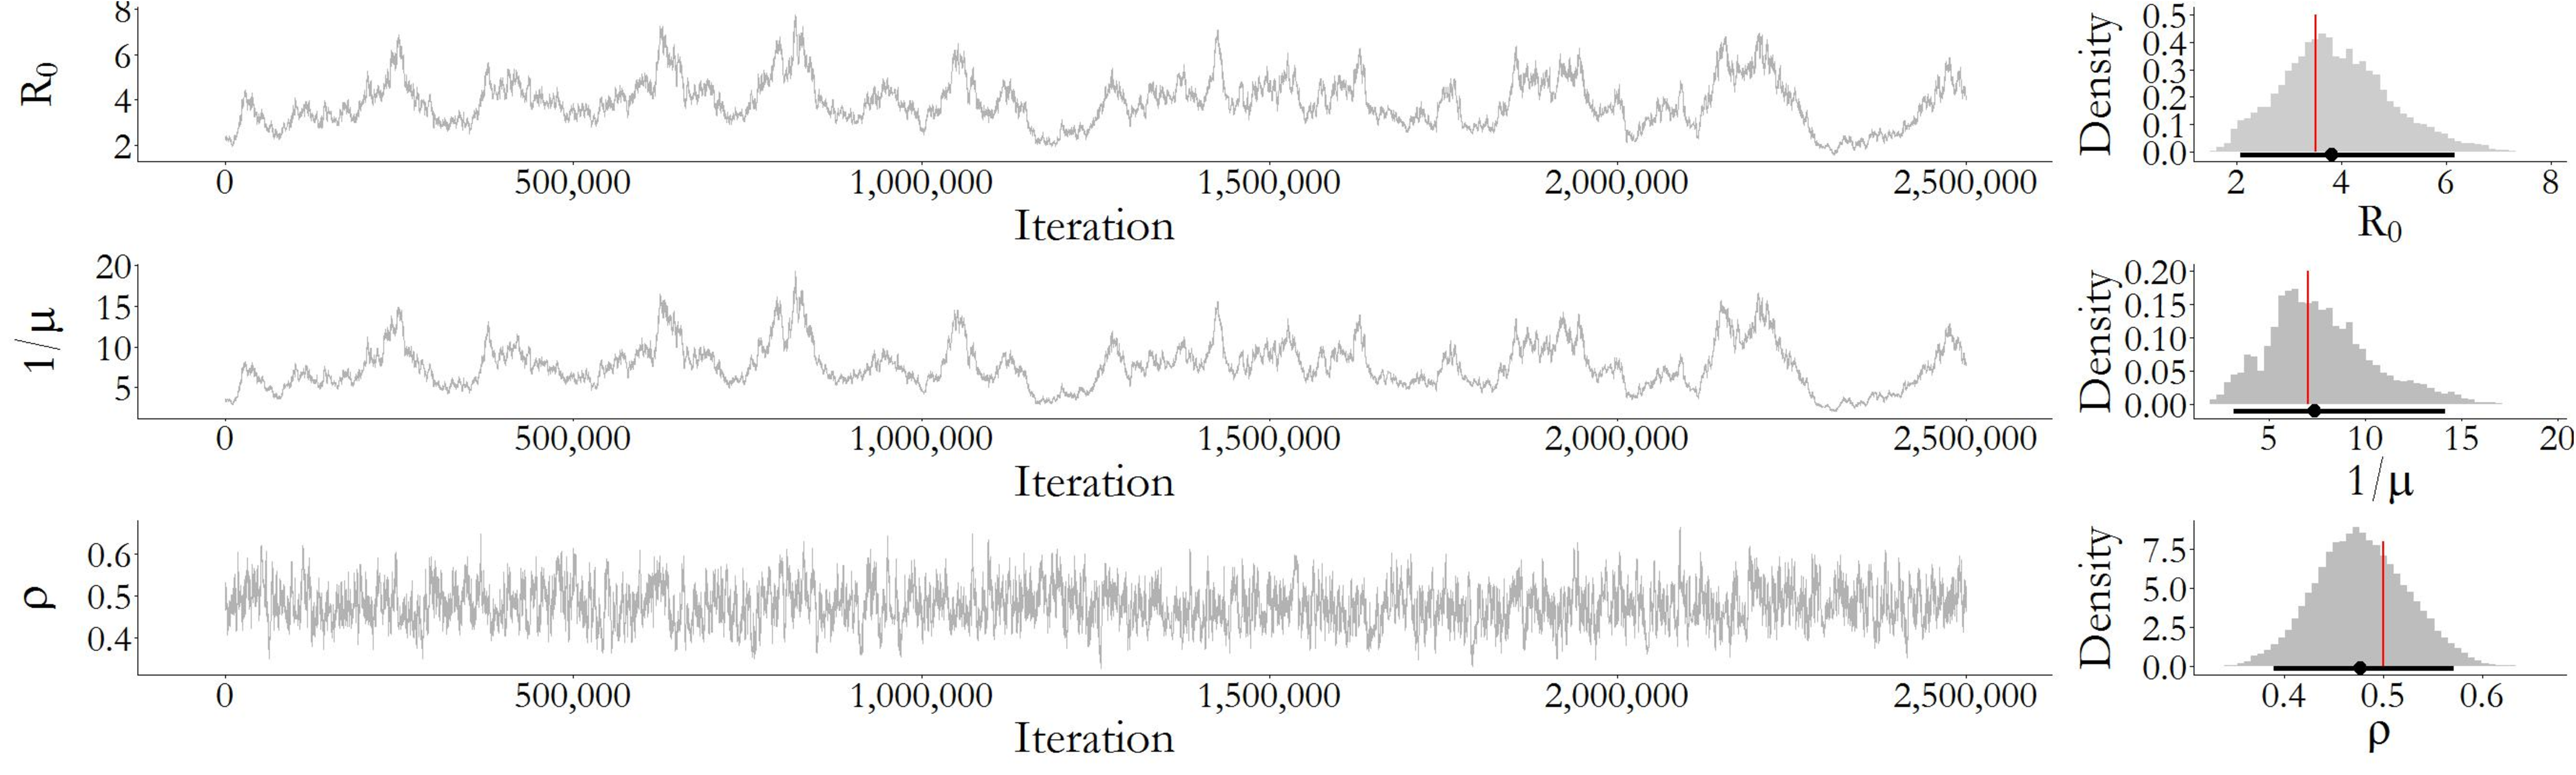
\includegraphics[width=0.9\textwidth]{figures/lna_centered_traces}
\caption[Traceplots for an MCMC chain using a centered LNA parameterization.]{Posterior traceplots for parameters of interest for a single MCMC chain of an SIR model fit to negative binomial distributed incidence data. MCMC targeted the posterior, \ref{eqn:lna_approximate_posterior}, alternately updating the non--restarting LNA for $ \bNtil|\btheta,\bY $ via elliptical slice sampling, and $ \btheta|\bNtil,\bY $ via a multivariate random walk Metropolis algorithm. $ R_0 = \beta N / \mu$ is the basic reproductive number, $ 1/\mu $ is the mean infectious period duration, and $ \rho $ is the mean case detection rate. The true values of $ R_0,\ 1/\mu,$ and $ \rho $ were 3.5, 7, and 0.5, respectively.}
\label{fig:lna_centered_traces}
\end{figure}

\subsubsection{Non--centered Parameterization}
\label{subsubsec:noncentered_parameterization}	

We can improve the mixing of our MCMC chains by reparameterizing the log--incidence process as a deterministic mapping of standard normal random variables, $ \bZ\sim MVN(\bs{0},\mb{I}) $, which are \textit{a priori} independent of the model parameters. Let $ \bNtil(t_\ell)\sim MVN(\bmu(t_\ell),\bSigma(t_\ell) $ and $ \bZ(t_\ell)\sim MVN(\bs{0},\mb{I}) $. Then the NCP is given by $ (\btheta,\bZ) $ and maps onto the CP via \begin{align}
\label{eqn:lna_ncp}
 \bNtil(t_\ell) \overset{\mcL}{=}\widetilde{\bW}(t_\ell),\ \widetilde{\bW}(t_\ell) = \bmu(t_\ell) + \bSigma(t_\ell)^{1/2}\bZ(t_\ell).
\end{align} We now target the joint posterior of the model parameters and the non--centered LNA draws,
\begin{align}
\label{eqn:lna_noncentered_posterior}
\pi(\btheta,\bZ|\bY) &\propto L(\bY|\doLNA(\bZ,\btheta,\mcI))\ind{\bN(\bZ,\btheta,\mcI)\in\mcS_N^R}\ind{\bX(\bZ,\btheta,\mcI)\in\mcS_X^R}\pi(\bZ)\pi(\btheta).
\end{align}
We will denote by $ \bN(\bZ,\btheta,\mcI) $ and $ \bX(\bZ,\btheta,\mcI) $ the incidence and prevalence sample paths that are output by the \doLNA\ procedure. The procedure for this mapping, denoted \doLNA, is presented in Algorithm (\ref{alg:doLNA}). 

\begin{algorithm}[htbp]
	\caption{Mapping standard normal draws onto LNA sample paths.}
	\label{alg:doLNA}
	\begin{algorithmic}[1]
		\Procedure{doLNA}{$ \bZ,\btheta,\mcI $}
		\State \textbf{initialize: }$ \bX(t_0) \gets \bX_0,\ \bN(t_0) \gets \bs{0},\ \bNtil(t_0) \gets \bs{0},\ \bmu(t_0) \gets \bs{0},\ \bSigma(t_0) \gets \bs{0} $
		\For{$ \ell = 1,\dots,L $}
		\State $ \bmu(t_\ell),\ \bSigma(t_\ell) \gets $ solutions to (\ref{eqn:lna_ode_drift}) and (\ref{eqn:lna_ode_diffusion}) over $ (t_{\ell-1}, t_\ell] $
		\State $ \bNtil(t_\ell)\gets \bmu(t_\ell) + \bSigma(t_\ell)^{1/2}\bZ(t_\ell) $ \Comment{non--centered parameterization}
		\State $ \bN(t_\ell)\gets \bN(t_{\ell-1}) + \exp(\bNtil(t_\ell)) - \bs{1} $
		\State \textbf{restart initial conditions:} 
		\State {\hspace{0.2in} $ \bX(t_\ell) \gets \bX(t_{\ell-1}) + \bA^T(\bN(t_\ell)-\bN(t_{\ell-1})),\ \bNtil(t_\ell) \gets \bs{0},\ \bmu(t_\ell)\gets\bs{0},\ \bSigma(t_\ell)\gets\bs{0} $ }
		\EndFor
		\State \hspace{-0.25in}\Return \Comment{return incidence and/or prevalence sample paths}
		\State$\bN = \left \lbrace\bN(t_0),\bN(t_1),\dots,\bN(t_L)\right \rbrace,\ \bX = \left \lbrace \bX(t_0),\ \bX(t_1),\dots,\bX(t_\ell) \right \rbrace $
		\EndProcedure
	\end{algorithmic}
\end{algorithm}

The NCP of the log--incidence process substantially improves the mixing of MCMC chains that alternate between updates to $ \bZ|\btheta,\bY $ and $ \btheta|\bZ,\bY $. Figure \ref{fig:lna_centered_traces} shows traceplots of model parameters for one of MCMC chains for an SIR model fit to Poisson distributed incidence data using the centered parameterization (CP) of the LNA transition density. MCMC was run for 2.5 million iterations, following a tuning run of equal length, but each chain only manages to yield a effective sample sizes for $ R_0 $ and the infectious period duration in the low double digits. In contrast, the NCP yields effective sample sizes per--chain of between 500--700 for each of the model parameters in only 50,000 iterations, following a short tuning run of equal length. Figure \ref{fig:lna_noncentered_traces} shows the traceplot for one of the MCMC chains, which clearly mixes better. 

\begin{figure}[htbp]
	\centering
	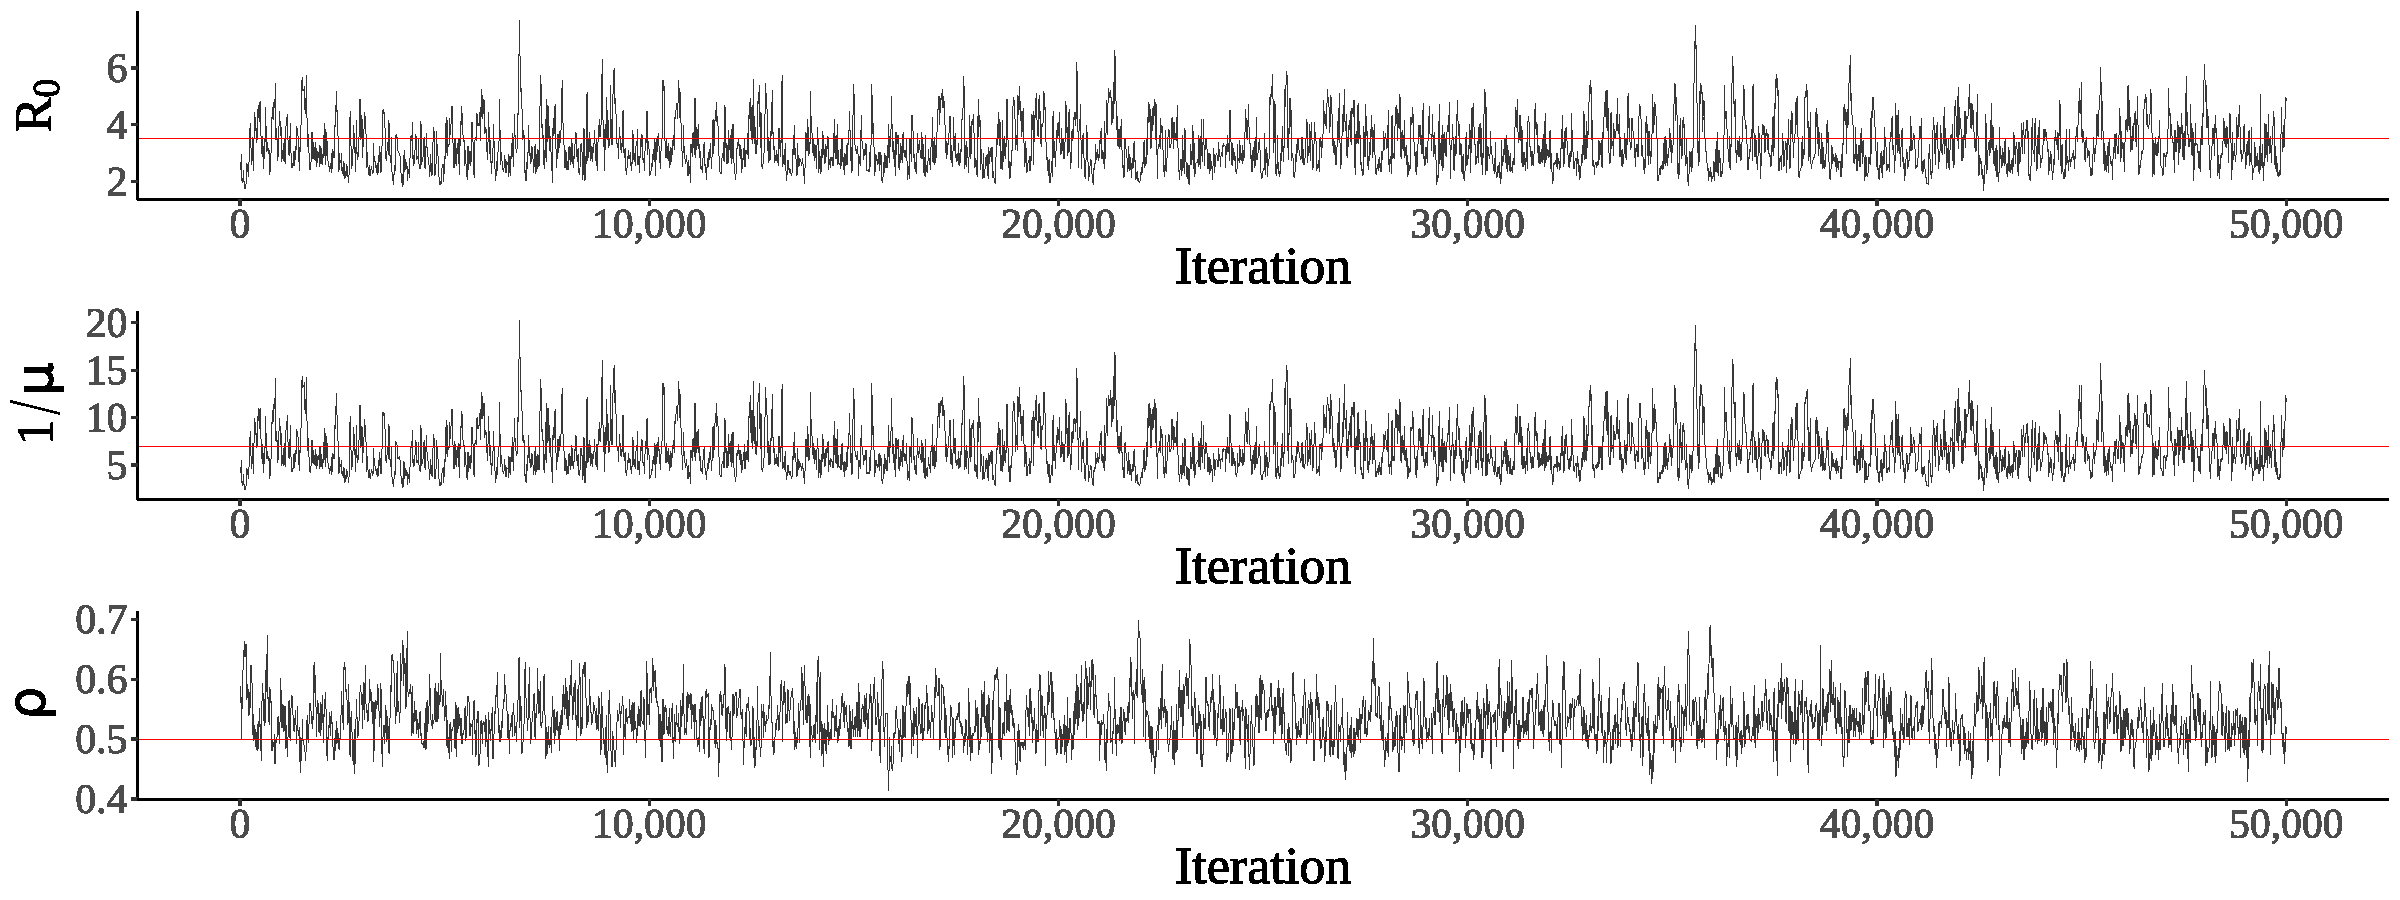
\includegraphics[width=0.9\textwidth]{figures/lna_noncentered_traces}
	\caption[Traceplots for an MCMC chain using a non--centered LNA parameterization.]{Posterior traceplots of parameters of interest sampled by a single MCMC chain of an SIR model fit to Poisson distributed incidence data. MCMC targeted the posterior, \ref{eqn:lna_noncentered_posterior}, alternately updating $ \bZ|\btheta,\bY $ via elliptical slice sampling, and $ \btheta|\bZ,\bY $ via a multivariate random walk Metropolis algorithm. $ R_0 = \beta N / \mu$ is the basic reproductive number, $ 1/\mu $ is the mean infectious period duration, and $ \rho $ is the mean case detection rate. The true values of $ R_0,\ 1/\mu,$ and $ \rho $ were 3.5, 7, and 0.5, respectively.}
	\label{fig:lna_noncentered_traces}
\end{figure}

In each iteration of a DA MCMC algorithm, we alternate between updates to the latent path, conditional on the model parameters, and updates to the parameters, conditional on the latent path. Figure \ref{fig:lna_sampling_diagram}, which depicts the CP and NCP representations of an LNA path, provides some insight into why the NCP improves MCMC mixing. Under the CP (top plot), updates to $ \btheta|\bNtil,\bY $ are made conditionally on a \textit{fixed} LNA path. Therefore, proposed parameter values are accepted depending on whether they are concordant with the data \textit{and} the current path. Even small perturbations to model parameters can result in shifts of the LNA transition densities (grey densities) that would render the current path (red points) unlikely under the proposal. In contrast, perturbations to parameters implicitly perturb the LNA path even as the LNA draws, $ \bZ $, are clamped to their current values. 

\begin{figure}[htbp]
	\centering
	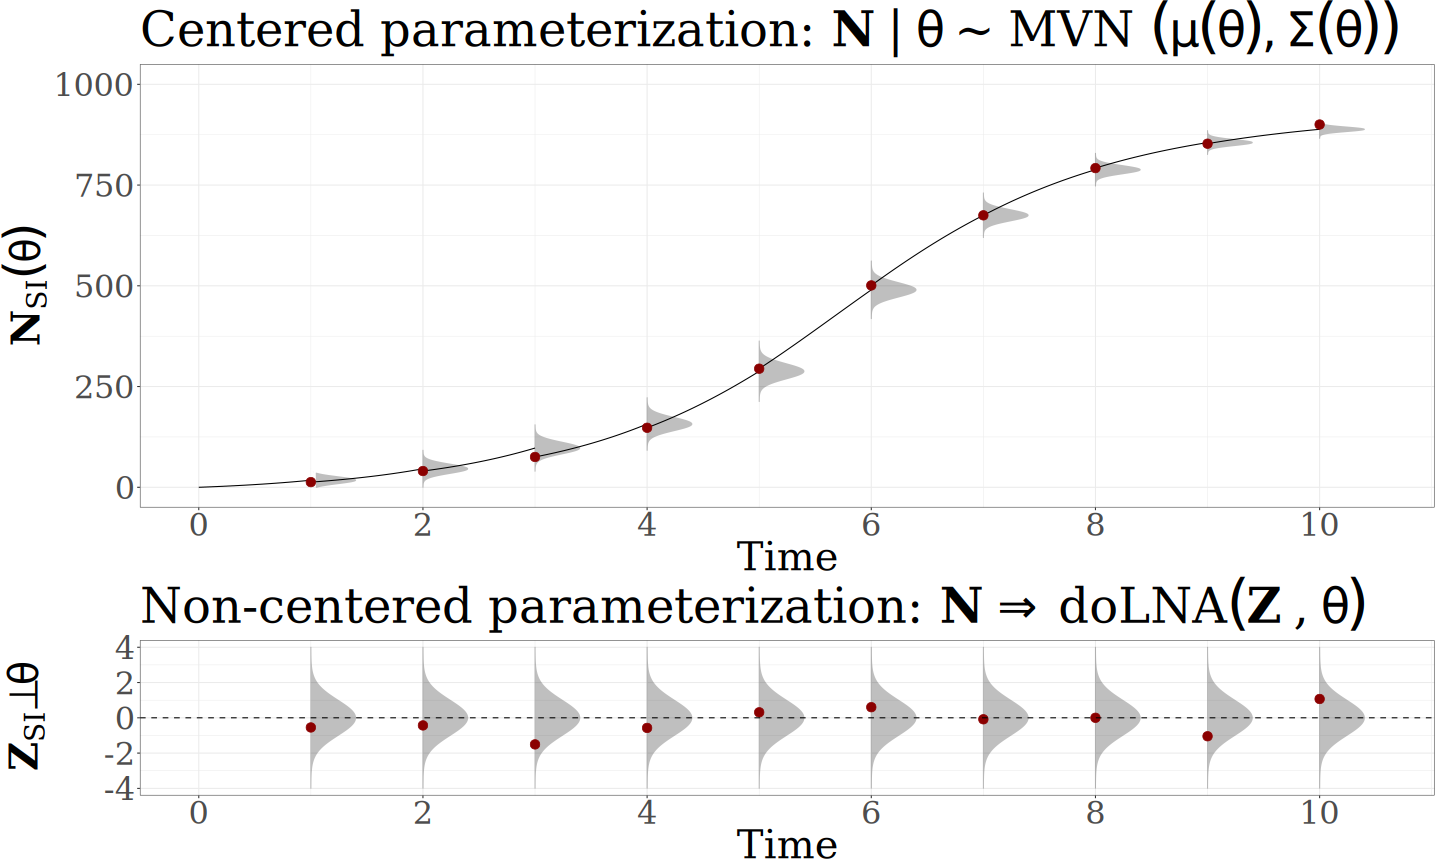
\includegraphics[width=0.9\textwidth]{figures/lna_sampling_diagram}
	\caption[Centered and non--centered LNA paths.]{Centered (top) and non--centered (bottom) parameterizations of an LNA incidence path. In the CP, the log--incidence is normally distributed with mean and covariance obtained by solving the LNA ODEs, (\ref{eqn:lna_ode_drift}) and (\ref{eqn:lna_ode_diffusion}). In the NCP, the log--incidence is a draw from a standard normal distribution that is deterministically mapped to a sample path via the $ \doLNA $ algorithm. In both the CP and NCP, state at the end of each interval determines the initial conditions of the LNA ODEs for the next interval. Plots of CP LNA transition densities are rescaled for clarity.}
	\label{fig:lna_sampling_diagram}
\end{figure}

The NCP of the LNA also plays an important role in facilitating efficient updates of $ \bZ|\btheta,\bY $ via the elliptical slice sampling (ElliptSS) algorithm of \cite{murray2010}, which was detailed in Section \ref{subsubsec:elliptical_slice_sampling} and is presented in Algorithm \ref{alg:elliptss_lna}. ElliptSS is an efficient and easy to implement MCMC algorithm for sampling latent Gaussian random variables, $ \bZ $, in models where the posterior of can be decomposed as the Gaussian prior for $ \bZ $ and an arbitrary likelihood, $ L(\bY|\bZ,\btheta) $, i.e.,
\begin{equation}
\label{eqn:eliptss_posterior_decomp}
\pi(\btheta,\bZ|\bY)\propto L(\bY|\bZ,\btheta)MVN(\bZ;\mu_\bZ,\bSigma_\bZ).
\end{equation}
The target posterior under the LNA NCP, (\ref{eqn:lna_noncentered_posterior}), is of this form, regardless of whether the LNA is restarted at the beginning of each inter--observation interval, as in \cite{fearnhead2014}, or the non--restarting version is used as in \cite{komorowski2009}. Note that the CP cannot be expressed as a jointly Gaussian collection of random variables with complete data likelihood of the form (\ref{eqn:eliptss_posterior_decomp}) when we use the restarting version of the LNA. Although each transition density, (\ref{eqn:lna_transition_density}), is itself Gaussian, the joint LNA path, $ \bN $, is not \textit{a priori} Gaussian when the LNA ODEs are restarted since the mean of $ \bN(t_\ell) $ depends non--linearly on the value of $ \bN(t_{\ell-1}) $. The quality of the LNA approximation is known to degenerate over long time intervals. Restarting the LNA ODEs has been established to improve the approximation when analyzing time series data of non--negligible length \cite{fearnhead2014,giagos2010inference,folia2017trajectory,minas2017long}. Hence, use of the NCP is critical to enabling the use of ElliptSS for jointly updating of $ \bZ|\btheta,\bY $ when using the restarting version of the LNA. 

We note that the elliptical slice sampling Algorithm \ref{alg:elliptss_lna} differs slightly from, but is equivalent to, the algorithm in \cite{murray2010} regarding how the initial proposal is made. The original algorithm was modified so that the distribution of angles for accepted proposals would be symmetric about zero in order to facilitate tuning of the initial bracket width. We have found that shrinking the initial bracket width often improves computational efficiency when fitting more complex models. This is discussed further in Section \ref{sec:lna_init_bracket_width}.

\begin{algorithm}[htbp]
	\caption{Sampling LNA draws via elliptical slice sampling.}
	\label{alg:elliptss_lna}
	\begin{algorithmic}[1]
		\Procedure{\doElliptSS}{$ \bZ_{cur},\btheta,\bY,\mcI,\omega = 2\pi $}
		\State Sample ellipse: $ \bZ_{prop} \sim N(\bs{0}, \mb{I}) $
		\State Sample threshold: $ u|\bx \sim \mr{Unif}(0, L(\bY|\doLNA(\bZ_{cur},\btheta,\mcI))) $
		\State Position the bracket and make initial proposal: \vspace{-0.1in}
		\begin{align*}
		\psi &\sim \mr{Unif}(0,\omega)\\
		L_\psi &\leftarrow -\psi;\ R_\psi \leftarrow L_\psi + \psi\\
		\phi &\sim \mr{Unif}(L_\psi,R_\psi)
		\end{align*}
		\State Set $ \bZ' \leftarrow \bZ_{cur}\cos(\phi) + \bZ_{prop}\sin(\phi) $. 
		\If{$ L(\bY|\doLNA(\bZ',\btheta,\mcI)) > u $}{ accept $ \bZ' $}
		\State\Return{ $ \bZ' $}
		\Else
		\State Shrink bracket and try a new angle:
		\State{\textbf{If:} $ \phi < 0 $}{ \textbf{then: }$ L_\phi \leftarrow\phi $ }{ \textbf{else: }$ R_\phi \leftarrow \phi $}
		\State $ \phi \sim \mr{Unif}(L_\phi, R_\phi) $
		\State \textbf{GoTo:} 5
		\EndIf
		\EndProcedure
	\end{algorithmic}
\end{algorithm}

\subsubsection{Initializing the LNA Draws}
\label{subsubsec:lna_init}
In simple models, reasonable parameter values will generally lead to valid LNA paths for initial $ \bZ\sim MVN(\bs{0},\mb{I}) $, i.e., paths that satisfy the monotonicity and positivity conditions, and thus have non--zero likelihood. However, this is not necessarily the case for complex models with many types of transition events, or when the time--series of incidence counts is long. One option is to include a re--sampling step after line 6 in Algorithm \ref{alg:doLNA}, in which $ \bZ(t_\ell) $ is redrawn in place until the conditions for a valid path over the interval are met. It is important to note that such a procedure does not sample from the correct distribution since $ \bZ $ is not actually a truncated multivariate Gaussian. To correct for this, we will ``warm--up" the LNA path with an initial run of ElliptSS iterations in which the likelihood only consists of the indicators for whether the path is valid. Note that ElliptSS, or any other valid MCMC algorithm for updating $ \bZ|\btheta,\bY $, will never lead to an invalid LNA path being accepted if the current LNA draws and model parameters correspond to a valid path. Similarly, updates to model parameters conditional on the LNA draws will also preserve the validity of LNA paths.

\subsubsection{Parameter Updates}
\label{subsubsec:lna_param_updates}
Each MCMC iteration will consist of a number of ElliptSS updates, typically one but possibly 2--3 for complex models, followed by a set of parameter updates. We will generally use either a global adaptive random walk Metropolis algorithm (Algorithm 4 in \cite{andrieu2008tutorial}) or the adaptive non--isotropic multivariate normal slice sampler (MVNSS) presented in Section \ref{subsubsec:slice_sampling}. In models where the initial state, $ \bX_0 $, is not fixed, we will assign a strongly informative prior $ \bX_0 \sim TMVN_{\mcS_X^R}\left (N\mb{p}, N(\diag(\mb{p}) - \mb{p}\mb{p}^T)\right ) $, which is a truncated multivariate normal approximation to a multinomial with initial state probabilities, $ \mb{p} $, constrained to the state space of compartment volumes. We update $ \bX_0 $ jointly with the LNA path via ElliptSS. Additional details are presented in Section \ref{sec:lna_init_volumes}.

We have found it helpful, for the purpose of assigning sensible priors to model parameters and for improving MCMC mixing and convergence, to parameterize the estimation scale on which the MCMC explores the parameter space in terms of how the parameters directly affect the model dynamics. For the SIR model, this might mean re-expressing the model parameters in terms of the basic reproductive number of an outbreak, $ R0 = \beta N /\mu $, and the recovery rate, $ \mu $. Additionally, we would like our estimation scale to be unconstrained and therefore sample (and either accept or reject) values for $ \log(R0) $ and $ \log(\mu) $. The importance of appropriately parameterizing the estimation scale is discussed at length in Section \ref{sec:est_scale_discussion}. 

\subsection{Implementation}
\label{subsec:lna_implementation}
The algorithms for approximate inference via the LNA and ODE models are implemented in the \texttt{stemr} $ \R $ package, which can be available, along with vignettes for reproducing our results, from the following stable GitHub repository: \texttt{https://github.com/fintzij/stemr}. The implementation is flexible and provides facilities for specification of arbitrary SEM dynamics, a variety of emission probability distributions, and capabilities for accommodating time--varying covariates, time--varying parameters, and deterministic forcings. Computationally intensive operations are implemented in \texttt{C++} via \texttt{Rcpp} and \texttt{RcppArmadillo} \cite{rcpp,rcpparmadillo}. ODE integration functions are dynamically compiled in \texttt{C++} with the help of the \texttt{odeintr} R package \cite{odeintr} and ODEs can be integrated using a variety of methods available in the \texttt{Odeint C++} library \cite{ahnert2011odeint}. Additional aspects of the implementation are discussed in Section \ref{sec:lna_implementation_vignettes}.

\section{Simulations}
\label{sec:lna_simulations}

\subsection{Motivating Use of the LNA --- Comparison with Common SEM Approximations}
\label{subsec:lna_coverage}

The LNA is by no means the only approximation of the transition density of the MJP representation of a SEM. In the following subsection, we will illustrate why the LNA is an attractive choice, balancing computational cost with fidelity of the MJP approximation. We benchmark the LNA against two commonly used approximations of the MJP: the deterministic approximation given by a system of deterministic ODEs that are the functional infinite population limit of the MJP \cite{fuchs2013inference}, and a discrete--time approximation of the MJP using a multinomial modification of the $ \tau $--leaping algorithm (MMTL) \cite{breto2011compound} to simulate epidemic paths within a particle marginal Metropolis--Hastings (PMMH) framework \cite{andrieu2010particle}. The ODE approximation was chosen because of its ubiquity in the study of epidemic modeling, while the MMTL approximation in combination with PMMH was chosen because of a straightforward and general implementation in the popular \texttt{pomp} package in \texttt{R} \cite{pompjss}. Arguably, the MMTL approximation is closer to the original MJP than the LNA since it preserves the discreteness of the latent state space, while the ODE approximation, being deterministic, is further removed from the MJP.

The fidelity of each approximation to the original MJP depends on the population size and the epidemic dynamics. In relative terms, outbreaks with explosive dynamics in large populations will tend to deviate less from their infinite population deterministic limits than outbreaks that occur in small populations, that are less contagious, or that are characterized by uncertainty in the probability and timing of a major outbreak. We fit SIR models to 500 datasets simulated under a range of SIR dynamics. Each dataset is simulated by drawing the model parameters from a set of prior distributions, simulating an outbreak via Gillespie's direct algorithm \cite{gillespie1976general}, and finally simulating the dataset as a negative binomial sample of the true incidence. Datasets arising from outbreaks that died off immediately were discarded and re--simulated, while datasets arising from outbreaks lasting longer than 50 epochs were truncated at 50 observations. SIR models were then fit via the LNA, ODE, and MMTL approximations under the priors from which the parameters were drawn. The simulation was repeated under three different regimes for the population size and the initial number of infected individuals, reflecting different levels of initial stochasticity in the epidemic trajectory. The priors and population sizes (Table \ref{tab:lna_coverage_sim}) were chosen because they were typical of settings in which the methods might reasonably be applied, e.g., the population sizes are not so big that the outbreaks would evolve deterministically, nor so small that the approximations would be unreasonable. All individuals who were not initially infected were susceptible at the start of each outbreak (i.e., no individuals with pre-existing immunity).  The population sizes and initial conditions were fixed at their true values. Hence, the only model misspecification was in the approximation used for the latent epidemic process. Additional results and details about the simulation setup are provided in Section \ref{sec:lna_coverage_supplement}. We also performed four analogous supplementary simulations, with similar results, where we generated datasets under fixed parameter regimes (presented in Section \ref{sec:lna_fixedpar_coverage}).

\begin{table}[htbp]
	\caption[LNA coverage simulation settings.]{Population sizes, initial conditions, and priors under which datasets were simulated. Five hundred datasets were simulated for each of the population size regimes. Each outbreak was simulated from a MJP with SIR dynamics. The observed incidence was a negative binomial sample of the true incidence in each inter--observation interval.}
	\label{tab:lna_coverage_sim}
	\footnotesize
	\centering
	\begin{tabular}{lccc}
		\hline
		& \textbf{Regime 1} & \textbf{Regime 2} & \textbf{Regime 3} \\\hline
		\textbf{Population size ($ N $)} & 10,000 & 50,000 & 250,000 \\ 
		\textbf{Initial infecteds ($ I_0 $)} & 1 & 5 & 25 \\
		\hline
		&&&
	\end{tabular} 

	\begin{tabular}{cllc}
		\hline
		\textbf{Parameter} & \textbf{Interpretation} & \textbf{Prior} & \textbf{Median (95\% Interval)} \\ \hline
		$ R0-1 $ & Basic reproduction \# - 1 & LogNormal(0, 0.5) & $ \implies R0 = $ 2.00 (1.38, 3.66) \\ 
		$ 1/\mu $ & Mean infectious period & LogNormal(-0.7, 0.35)& 1.43 (0.72, 2.84) \\
		$ \rho / (1-\rho) $ & Odds of case detection & LogNormal(0, 1) & $ \implies \rho =$ 0.5 (0.12, 0.88) \\
		$ \phi $ & Neg.Binom. over--dispersion & Exponential(0.1) & 6.93 (0.25, 36.89)\\
		\hline
	\end{tabular}
\end{table}

\subsubsection{Results}

This simulation was designed to be generous to the approximations that were used in fitting SEMs to the simulated data. The initial compartment counts and true population sizes were known, and there was no misspecification with respect to either the sampling model or the epidemic dynamics. Despite this, the ODE models struggle to reliably recover the true parameters, particularly those governing the sampling process. As shown in Figure \ref{fig:lna_coverage_main}, coverage of credible intervals for ODE models was low for all model parameters, and this was only somewhat mitigated as the population size increased. Coverage of credible intervals for models fit via the LNA and via MMTL were close to the nominal 95\% levels for all model parameters in all three population size regimes. The distributions LNA point estimates and credible intervals were also similar to MMTL point estimates and credible intervals for all parameters at all three population sizes. Further inspection of the relative posterior median deviations indicate that the ODE estimates are less precise, and credible interval widths tend to be narrower than credible intervals obtained with the two stochastic approximations. This is in agreement with findings by other authors who have found that ODE models tend to underestimate uncertainty in epidemic dynamics (see e.g., \cite{king2015avoidable}). Taken together, these results suggest that the LNA is, at least in this simple example, about as good at approximating the original MJP as is the more exact MMTL. 

\begin{figure}[htbp]
	\begin{fullpage}
		\centering
		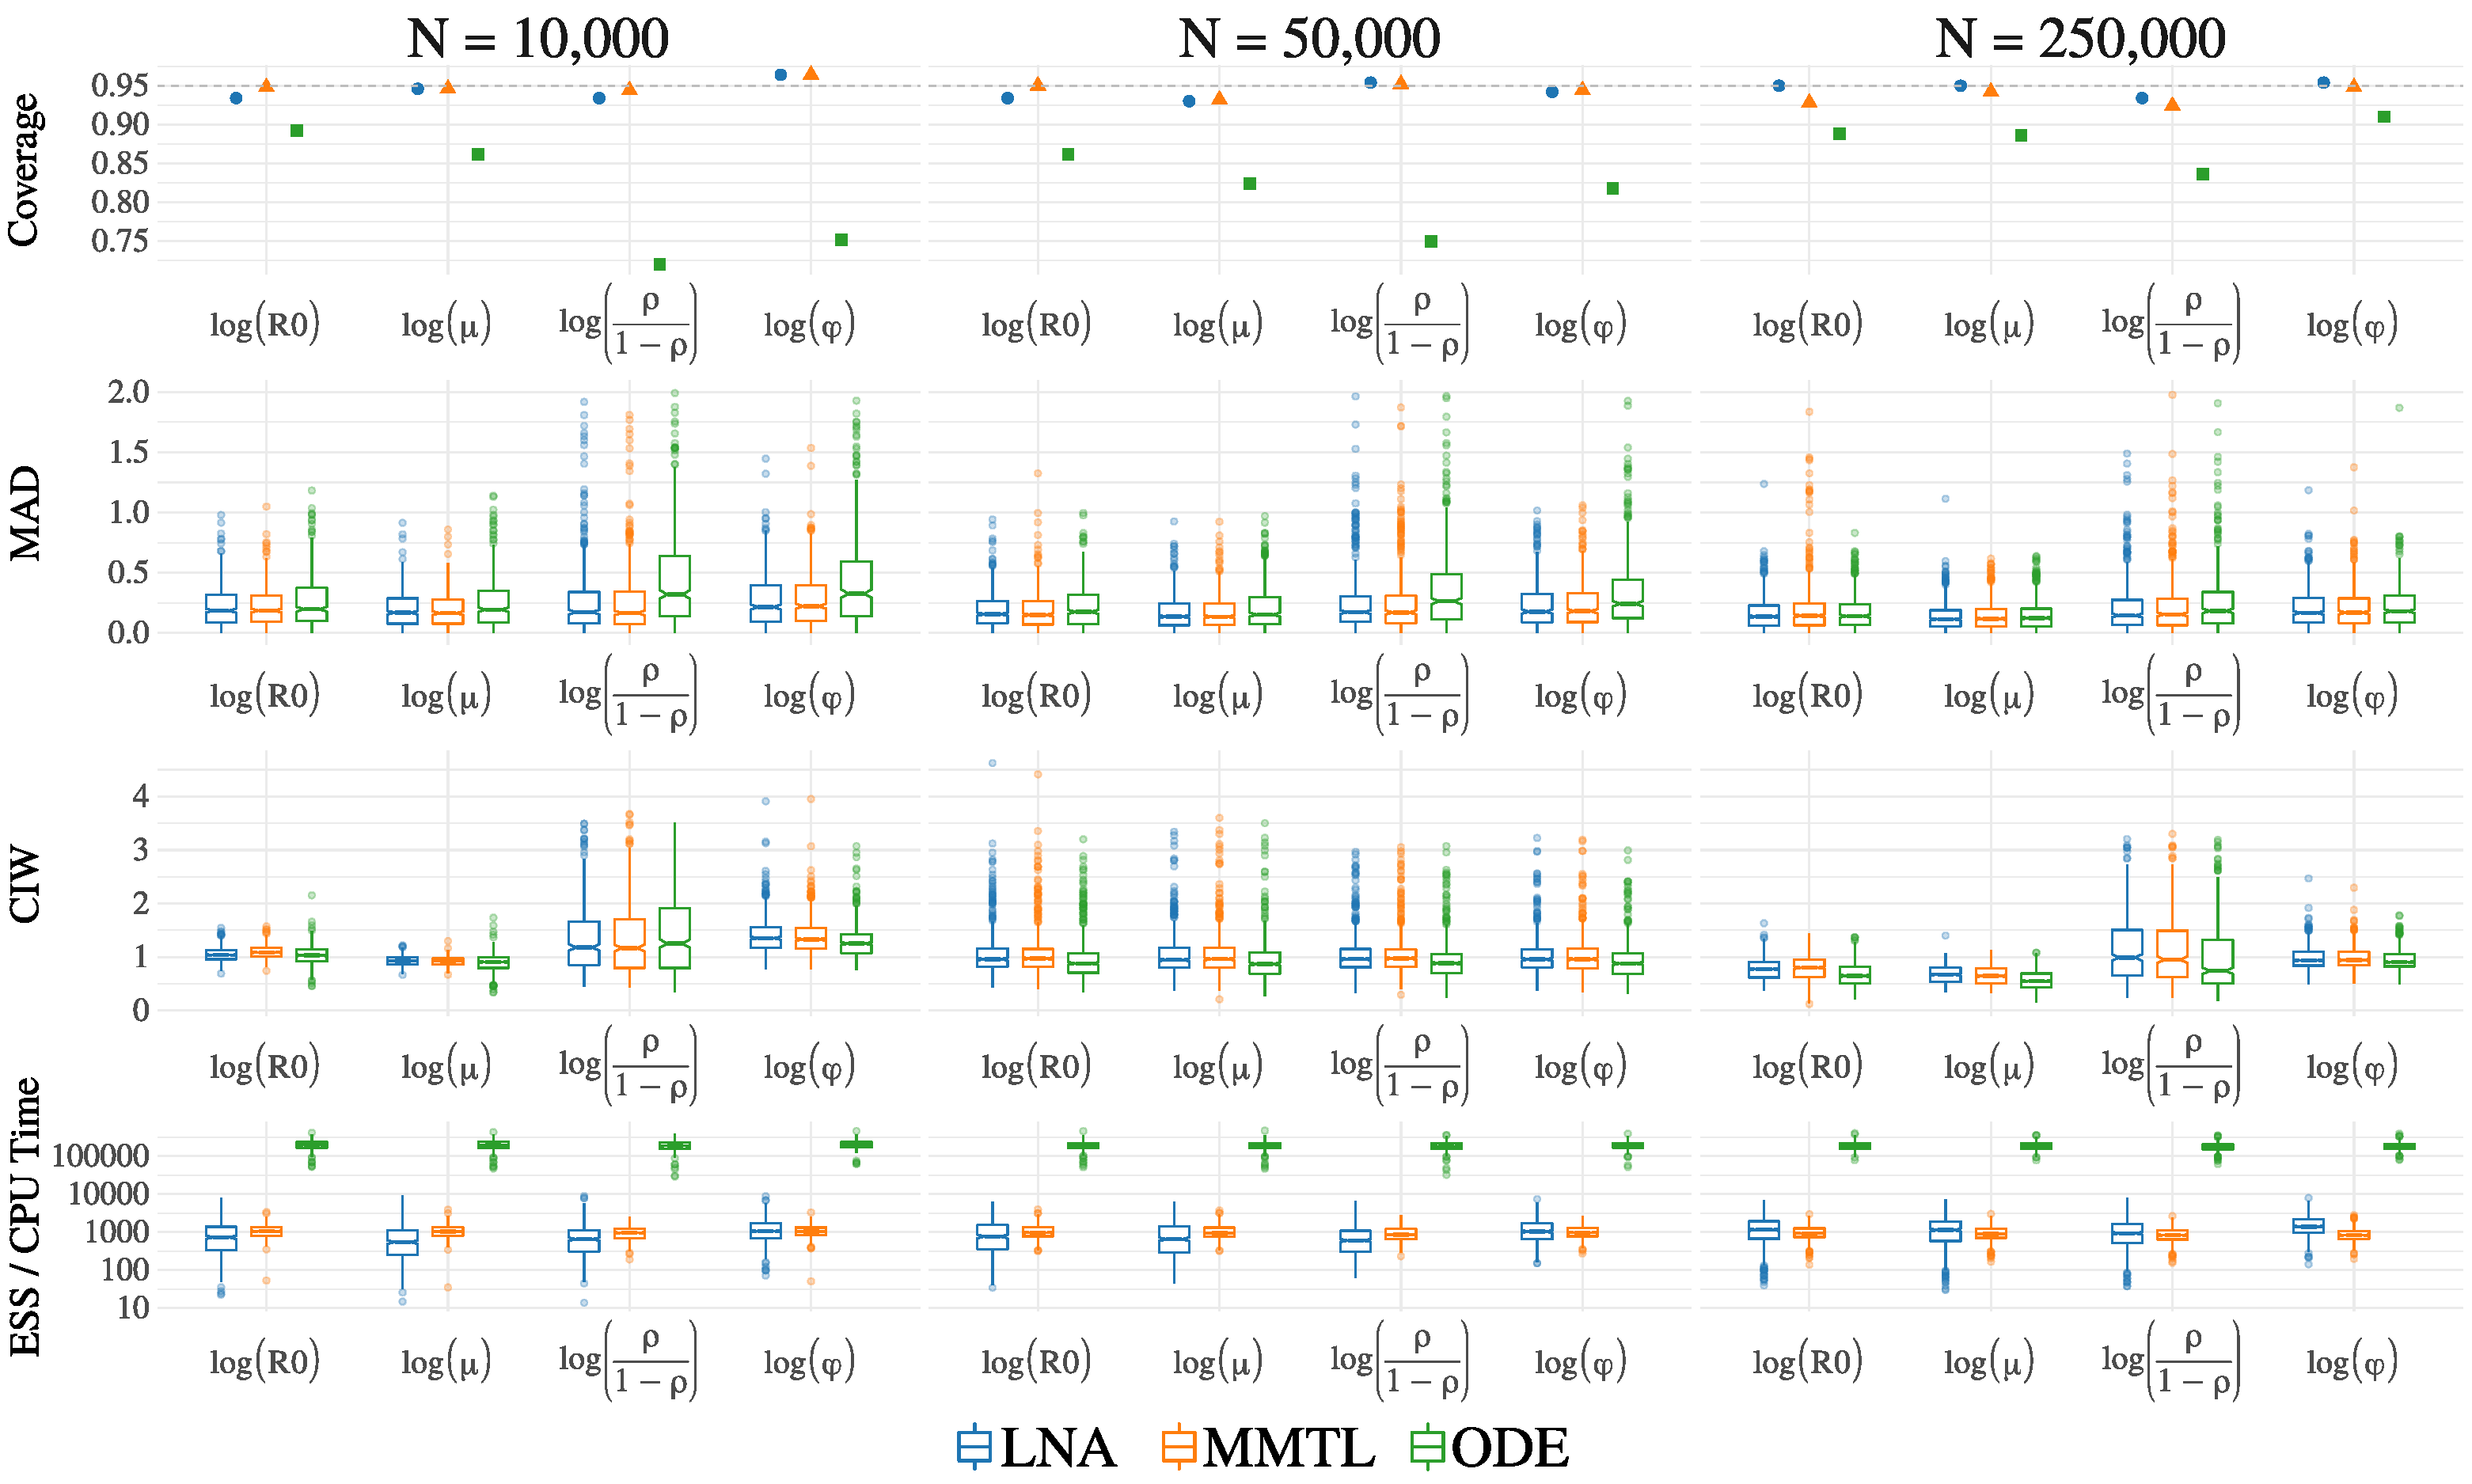
\includegraphics[width=\textwidth]{figures/lna_coverage_plots_main}
		\caption[Coverage simulation results for SIR models fit via the LNA, ODE, and MMTL approximations.]{Comparison of posterior results for SIR models fit to 500 datasets via the linear noise approximation (LNA), multinomial modified $ \tau $--leaping (MMTL) within particle marginal Metropolis--Hastings, and deterministic ordinary differential equations (ODE). $ R_0 $ is the basic reproductive number of an outbreak, $ \mu $ is the recovery rate, $ \rho $ is the negative binomial case detection probability, $ \phi $ is the negative binomial over--dispersion parameter. The rows correspond to the proportion of runs where the 95\% Bayesian credible interval covered the true parameter values, the posterior median deviation (PMD), the median absolute deviations of ODE and LNA models relative to MMTL (Rel. MAD), the 95\% Bayesian credible interval widths (CIW), and the widths of 95\% Bayesian credible intervals of ODE and LNA models relative to MMTL (Rel. CIW). The simulation was repeated for three regimes of population sizes and initially infected individuals (columns).}
		\label{fig:lna_coverage_main}
	\end{fullpage}
\end{figure}

We note that these results are not intended to suggest that there is no place for ODE models in the computational toolbox of disease modelers. To the contrary, when time is of the essence, as in an outbreak setting, crude estimates via the ODE may be obtained quickly. Average ODE run times were substantially shorter than LNA and MMTL run times and required far less CPU time per effective sample (see Table \ref{tab:lna_coverage_compstats}). ODE models are also appealing because they lend themselves to analytic characterizations of various aspects of the outbreak dynamics, e.g., relating the final outbreak size to the basic reproductive number (see, e.g., \cite{andersson2000stochastic,britton2018,keeling2008}).

In this simple simulation, the LNA and MMTL approximations had comparable computational performance, with the LNA perhaps being somewhat faster, but also with the caveat that comparing the ODE/LNA approximations with the MMTL approximation on the basis of computational performance is a bit misleading since the comparison would have turned out differently had we made other choices for the LNA and MCMC settings (e.g., timestep of MMTL, number of particles in PMMH, or tuning the initial EllipSS bracket width for the LNA). The important point to make regarding computational performance is that as model dynamics get more complex and the time series get longer, approximations, such as MMTL, that are used within a particle filter framework, such as PMMH, will become computationally infeasible. In many cases, the lack of an adequate model from which to simulate particle paths will lead to issues of particle degeneracy and an inability to fit even simple models (see \cite{fintzi2017efficient} for an example). Indeed, PMMH was abandoned as a computational strategy for analyzing Ebola data in later sections because of difficulty fitting SEMs with reasonable effort. However, as we shall see in the following sections, the LNA remains performant even as the model dynamics increase in complexity. 
 
 \begin{table}[htbp]
 	\caption[Computational performance of the ODE, LNA, and MMTL approximations.]{Run times, effective sample sizes, and relative geometric mean (GM) log--posterior effective sample size (ESS) per CPU time for models fit via the ODE, LNA, and MMTL approximations. Run times and ESS are computed over all chains. The GM log--posterior ESS/CPU time was computed over the five chains for each model and divided by the corresponding GM ESS/CPU time for the MMTL model. We report 50\% (2.5\%, 97.5\%) quantiles of the CPU time, ESS, and relative GM ESS/CPU time.}
 	\label{tab:lna_coverage_compstats}
 	\footnotesize
 	\centering
 	\begin{tabular}{lccc}	
 		\hline	
 		& \textbf{ODE} & \textbf{LNA} & \textbf{MMTL} \\\hline
 		\textbf{CPU time (minutes)} &  0.42 (0.23, 0.64) & 27.78  (12.03, 56.25) & 86.96 (40.47, 159.68) \\ 
 		\textbf{Effective sample size} & 5745 (4557, 6616) & 4067   (346, 11313) & 6834 (3764, 11879) \\
 		\textbf{GM ESS/CPU time vs. MMTL} & 180 (90, 350) & 1.87 (0.14, 8.84) & --- \\
 		\hline
 		&&&
 	\end{tabular} 
 \end{table}

\subsection{Assessing Model Fit}
\label{subsec:lna_model_diags}

Although model assessment is not the focus of this work, we emphasize the importance of diagnostics and briefly present several in--sample diagnostic tools that can be used to interrogate SEMs fit via the LNA. We highlight the following diagnostics because they are easily implemented post-hoc and require little effort beyond caching random quantities throughout the MCMC run. We do not delve into out--of sample diagnostics that could be used to assess the utility of a model for forecasting because proper predictive diagnostics involve recursively re--fitting the model and forecasting new data (see \cite{paul2011predictive,held2018forecasting}). This is infeasible in our setting due to the computational burden of fitting each model.

One of the central objectives in infectious disease modeling is to estimate the severity and duration of an outbreak \cite{lofgren2014opinion}. However, the true epidemic path is not observed so it is impossible to check whether it is captured by the latent posterior. This, of course, assumes that the latent process is itself identifiable, which may not be the case when estimating the effective population size (this is discussed in \ref{sec:effpop_identifiability}). Similarly, we cannot typically check that the distribution of expected observed incidence actually captures the true mean incidence we would expect to observed in we knew the true incidence (note that $ \rho\bN_\mr{true} $ is always identifiable in the models we consider). A standard alternative is to check whether the observed incidence is captured in the posterior predictive distribution. 

The partial posterior predictive distribution, shown in the middle plot of Figure \ref{fig:sirdiagplots}, is the predicted observed incidence, conditional on the outbreak being distributed according to the epidemic paths that we believe to be likely given the data at hand (i.e. the latent posterior). Here, new data are sampled using the posterior distribution of the observation model conditionally on the paths in the latent posterior sample. Hence, for replication $ j $, we simulate \begin{equation}
\label{eqn:lna_partial_postpred}
Y_{\ell,rep}^{(j)}|\bN_{post}^{(j)},\btheta_{post}^{(j)} \sim \mr{Neg.Binom.}\left (\mu = \rho^{(j)}\left (N_{SI}^{(j)}(t_\ell) - N_{SI}^{(j)}(t_{\ell-1})\right ),\sigma^2 = \mu + \mu^2 / \phi^{(j)} \right ),
\end{equation} 
where $ \bN_{post}^{(j)} $ and $ \btheta_{post} $ are the $ j^{th} $ posterior samples for the latent path and model parameters. 

The full posterior predictive distribution, shown in the right plot of Figure \ref{fig:sirdiagplots}, is the predicted observed incidence, integrated over the predicted latent incidence given the current data. Under the full posterior predictive distribution, new data are sampled by simulating a new latent path under the posterior distribution of the epidemic model parameters, and then simulating a new dataset conditionally on the simulated path. So, for replication $ j $, we simulate \begin{align}
\label{eqn:lna_full_postpred}
\bZ^{(j)}_{rep} &\overset{i.i.d.}{\sim} N(0,1),\ \bN^{(j)}_{rep} = \doLNA(\bZ^{(j)}_{rep},\btheta_{post}^{(j)},\mcI), \\ 
Y_{\ell,rep}^{(j)}|\bN_{rep}^{(j)},\btheta_{post}^{(j)} &\sim \mr{Neg.Binom.}\left (\mu = \rho^{(j)}\left (N_{SI}^{(j)}(t_\ell) - N_{SI}^{(j)}(t_{\ell-1})\right ),\sigma^2 = \mu + \mu^2 / \phi^{(j)} \right ),
\end{align} 
where $ \bZ_{rep}^{(j)} $ is a new vector of LNA draws. 

The full posterior predictive distribution provides a diagnostic for whether the joint model for the latent epidemic process and the observation process is reasonable as a data generating mechanism. In contrast, the partial posterior predictive distribution is useful for qualitatively assessing the adequacy of the emission distribution. Note that, when simulating from the full posterior predictive distribution, the replicated paths must still satisfy the constraints on the state space of $ \bN $ and $ \bX $. We can sample from the approximate posterior predictive distribution using the procedure described in Section \ref{subsubsec:lna_init} to avoid rejection sampling. 
\begin{figure}[htbp]
	\centering
	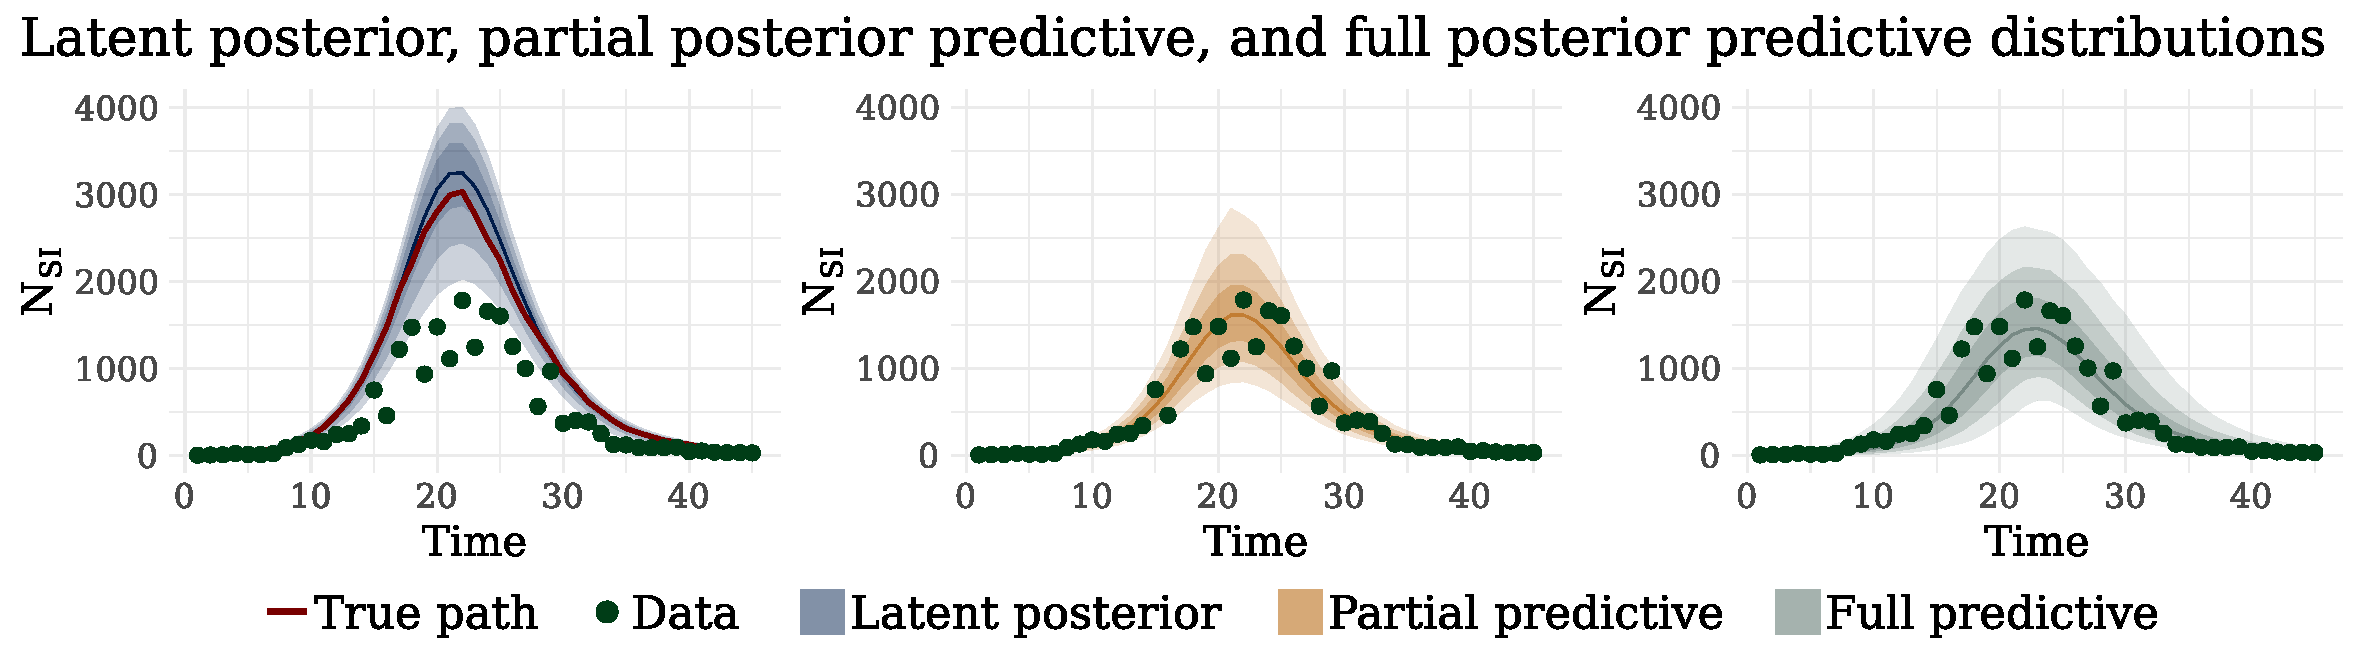
\includegraphics[width=\linewidth]{figures/sir_diag_plots}
	\caption[SIR model posterior incidence, posterior mean observed incidence, partial posterior predictive, and full posterior distributions.]{From left to right, the posterior incidence, posterior mean observed incidence, partial posterior predictive, and full posterior predictive distributions. The true incidence is the dashed red line in the leftmost plot and the observed incidence counts are the solid green dots in the right two plots. The solid red line is the true mean observed incidence, given by the true incidence multiplied by the case detection probability. The shaded bands, in order of lightest to darkest, correspond to pointwise posterior 95\%, 80\%, and 50\% credible intervals, with the pointwise posterior median given by the corresponding colored solid line.}
	\label{fig:sirdiagplots}
\end{figure}

In addition to validating a particular model, we can also use posterior predictive distributions to compare models. Figure \ref{fig:sinfoi_ppi_comp_diag} compares posterior predictive p--values (PPPs) and relative posterior predictive interval (PPIs) widths for two SIRS models (discussed further in Section \ref{subsec:tparam_motivation}) that were fit to data generated from an SIRS model with time--varying dynamics. The posterior predictive distribution of the more flexible model, which assigned a Gaussian Markov random field shrinkage prior to the time--varying basic reproduction numbers in the model,  produces more accurate predictive intervals (most PPPs between 0.25 and 0.75, and fewer PPPs near 0 or 1) has substantially narrower PPI widths (almost all dots are red, many are dark red). 

\begin{figure}[htbp]
	\centering
	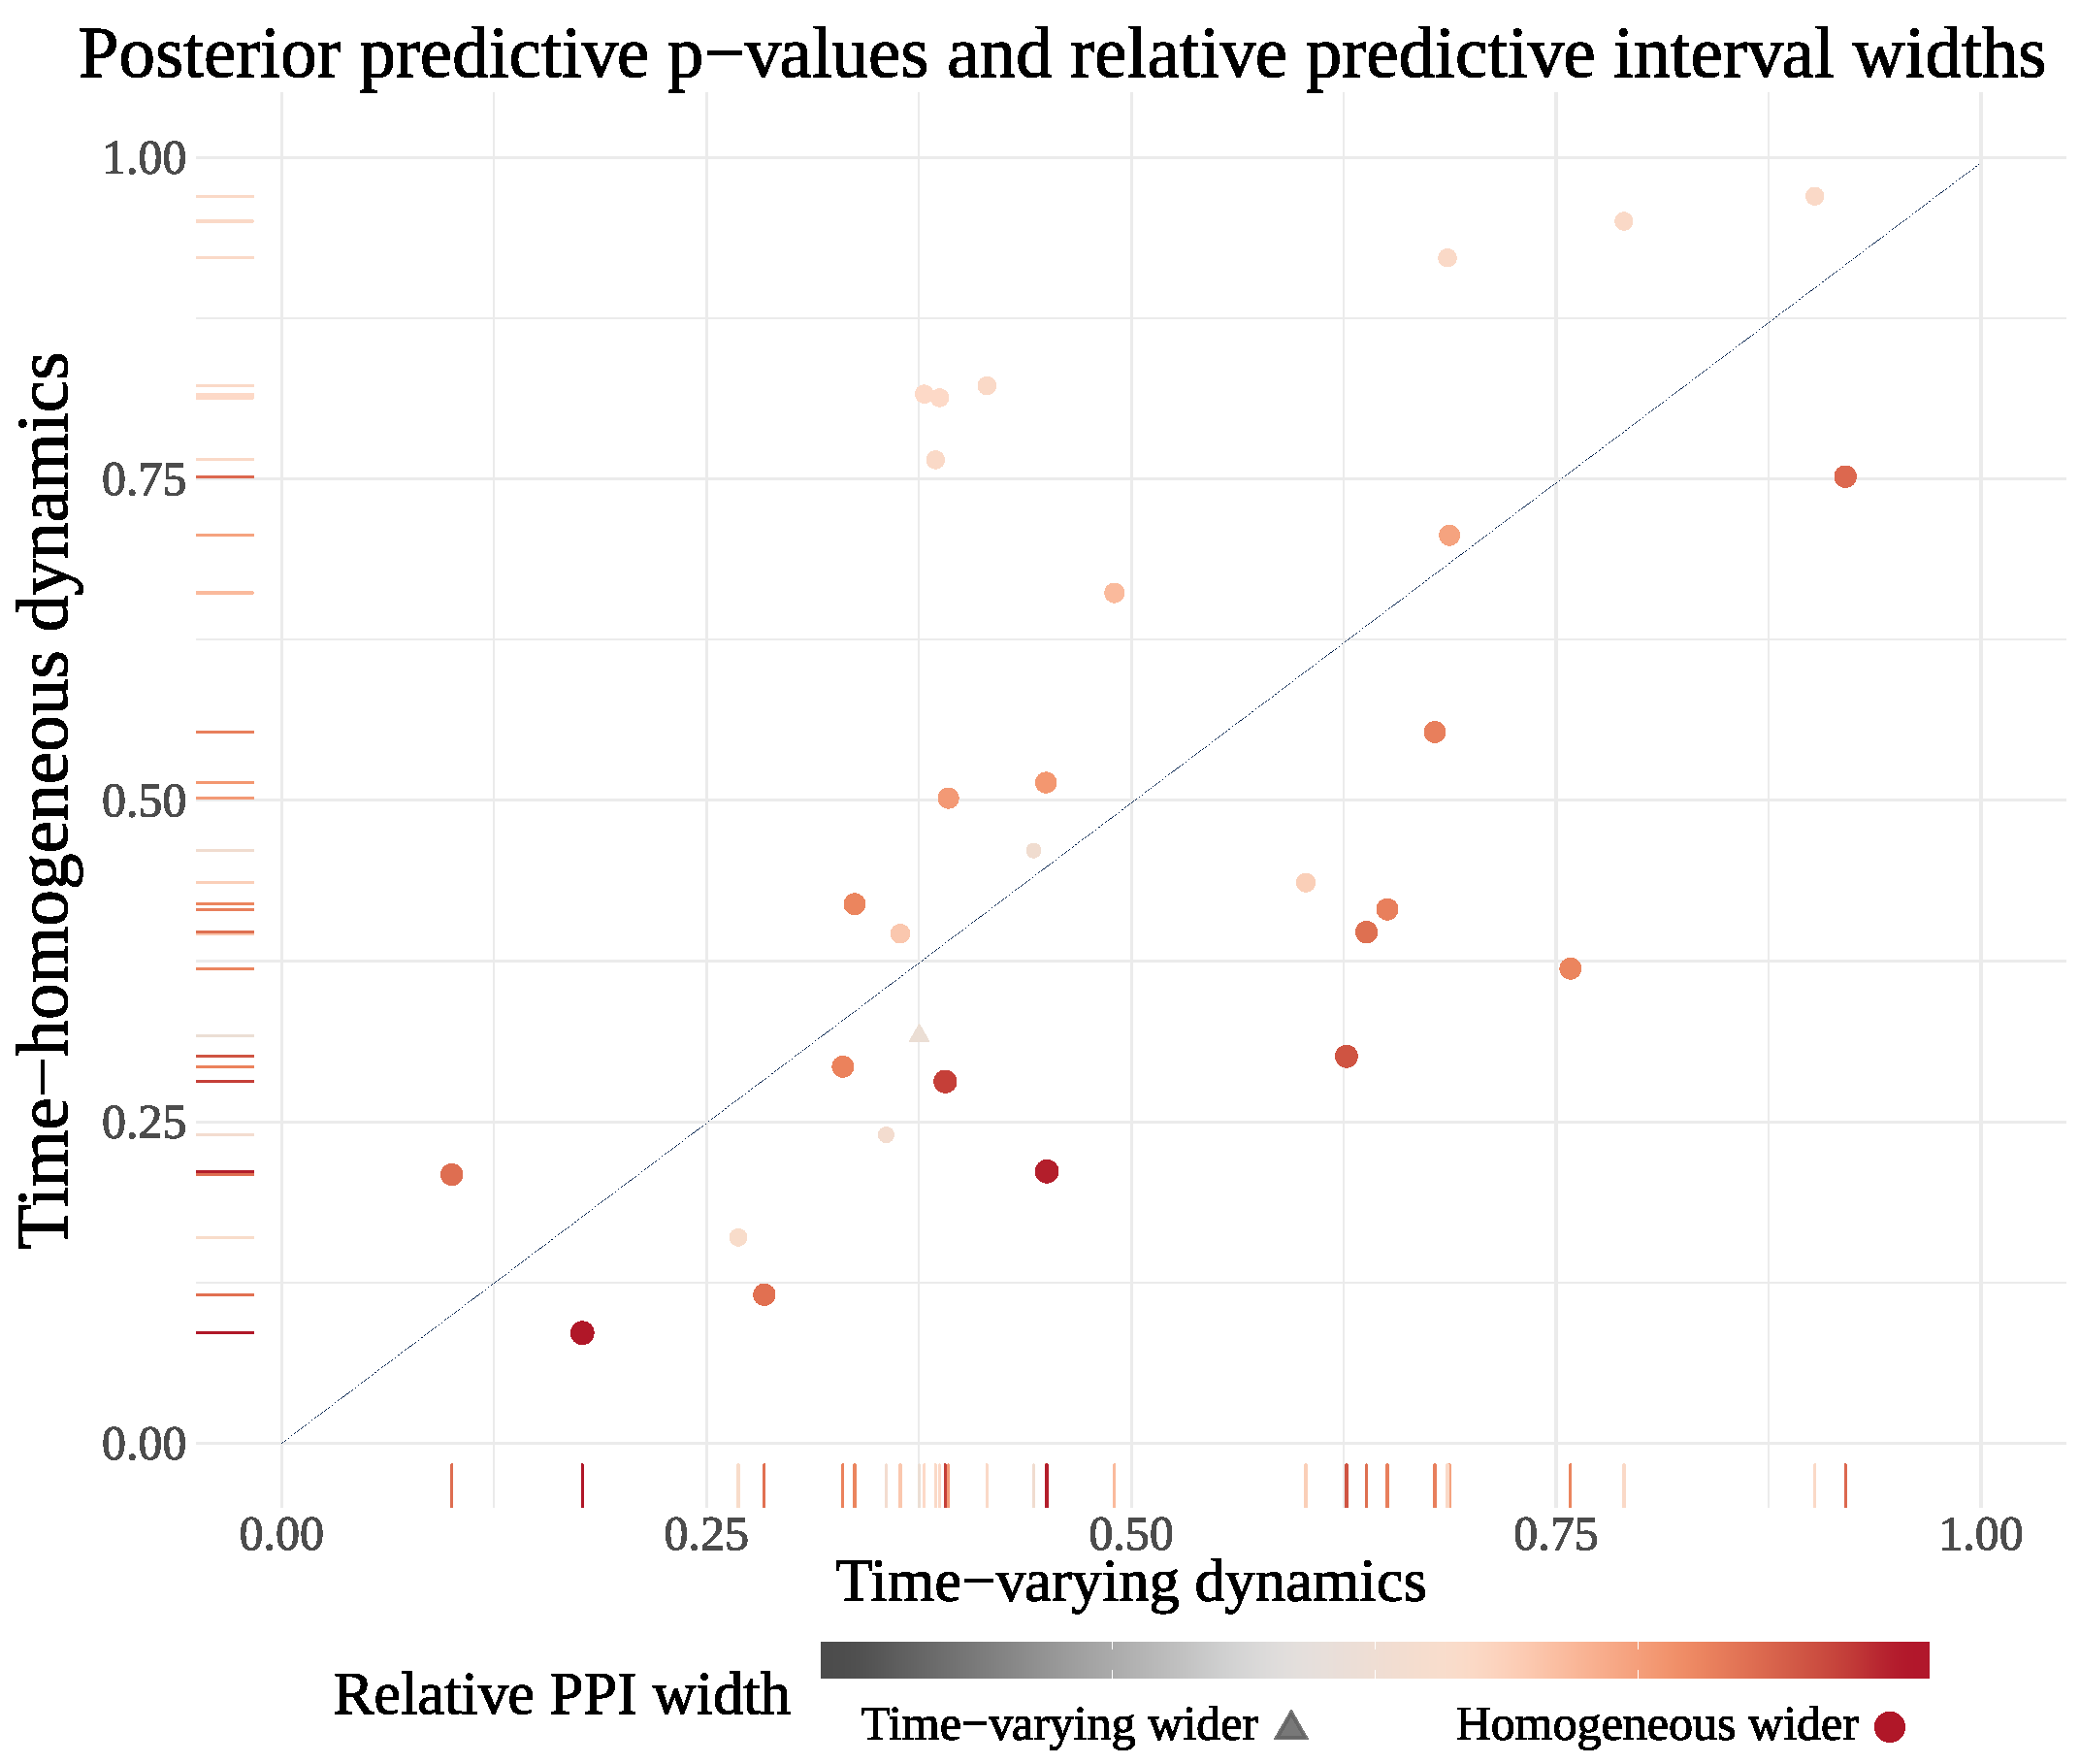
\includegraphics[width=0.85\linewidth]{figures/sinfoi_ppi_comp}
	\caption[Model comparison with posterior predictive p-values and relative predictive interval widths.]{Comparison of models with time--varying and constant force of infection using posterior predictive p-values (PPPs) and relative posterior predictive interval (PPI) widths. Each point corresponds to the observed incidence in a given week. The X--Y coordinates give the PPPs under a model with a time--varying force of infection (FOI), where R0 was modeled as a Gaussian Markov random field of order one, the PPP under a model with constant per--contact infection rate. The size and color of each point corresponds to the relative PPI width, computed as $ (\widehat{\sigma}_{post,\ell}^{constant} - \widehat{\sigma}_{post,\ell}^{RW1})/\widehat{\sigma}_{post,\ell}^{RW1} $, and the sign of the relative width is further emphasized by the shape of the point. Dots indicate that PPIs with constant FOI are wider, the lone triangle corresponds to the one data point where the PPI for the model with time--varying FOI was wider.}
	\label{fig:sinfoi_ppi_comp_diag}
\end{figure}

We are also interested in understanding the extent to which the data (and boundary conditions on the latent process) suggest that there should be an excess or dearth of infections and recoveries beyond what we would expect under the LNA prior. Figure \ref{fig:sir_drawplots} shows the posterior distributions of LNA draws for an SIR model, along with theoretical quantiles of the posterior predictive distribution and empirical quantiles of the posterior predictive distribution, accounting for boundary conditions. The distribution in each interval, $ \mcI_\ell $, is shaded by the posterior shrinkage, defined as $ s_\ell = 1 - \sigma_\ell$, where $ \sigma_\ell $ is the posterior standard deviation of the LNA draws over $ \mcI_\ell $. Note that the posterior predictive distribution is the same as the LNA prior.

To the extent that the emission distribution is correctly specified, discrepancies between the prior and posterior distributions of LNA draws can point to intervals where the data are informative, intervals over which the prior and posterior are in conflict, or possibly a combination of influential observations and model misspecification. An important feature of the NCP of the LNA transition density is that it standardizes the latent posterior so that we can interpret contractions of the posterior, vis--a--vis the LNA prior, as pointing to intervals where the data add information. Shifts of the posterior, absent contraction, point to intervals over which the model dynamics do not explain the observed incidence. If we were to examine the CP of the LNA posterior, it would be difficult to identify shifts and contractions due to the mean--variance relationship of LNA transition densities.

Figure \ref{fig:sir_drawplots} shows pronounced shifts and contractions at the beginning and end of the outbreak. During those periods, the MJP used to simulate the outbreak is both far from its deterministic limit and is not yet well approximated by the LNA. Data at the start of the outbreak are also highly informative about the timing and intensity of the exponential growth phase of the epidemic, and hence its dynamics. In contrast, during the exponential growth and decay of the outbreak, the LNA posterior is concordant with the prior. At times when we observe a contraction with little shift in the posterior, we would conclude that the data are informative but do not suggest model misspecification. Finally we note that the boundary conditions on the latent state space have little effect the posterior predictive distribution of the latent process, except at the beginning of the outbreak (though if we would expect to see similar behavior if we extended the right tail of the observation window). 


\begin{figure}[htbp]
	\centering
	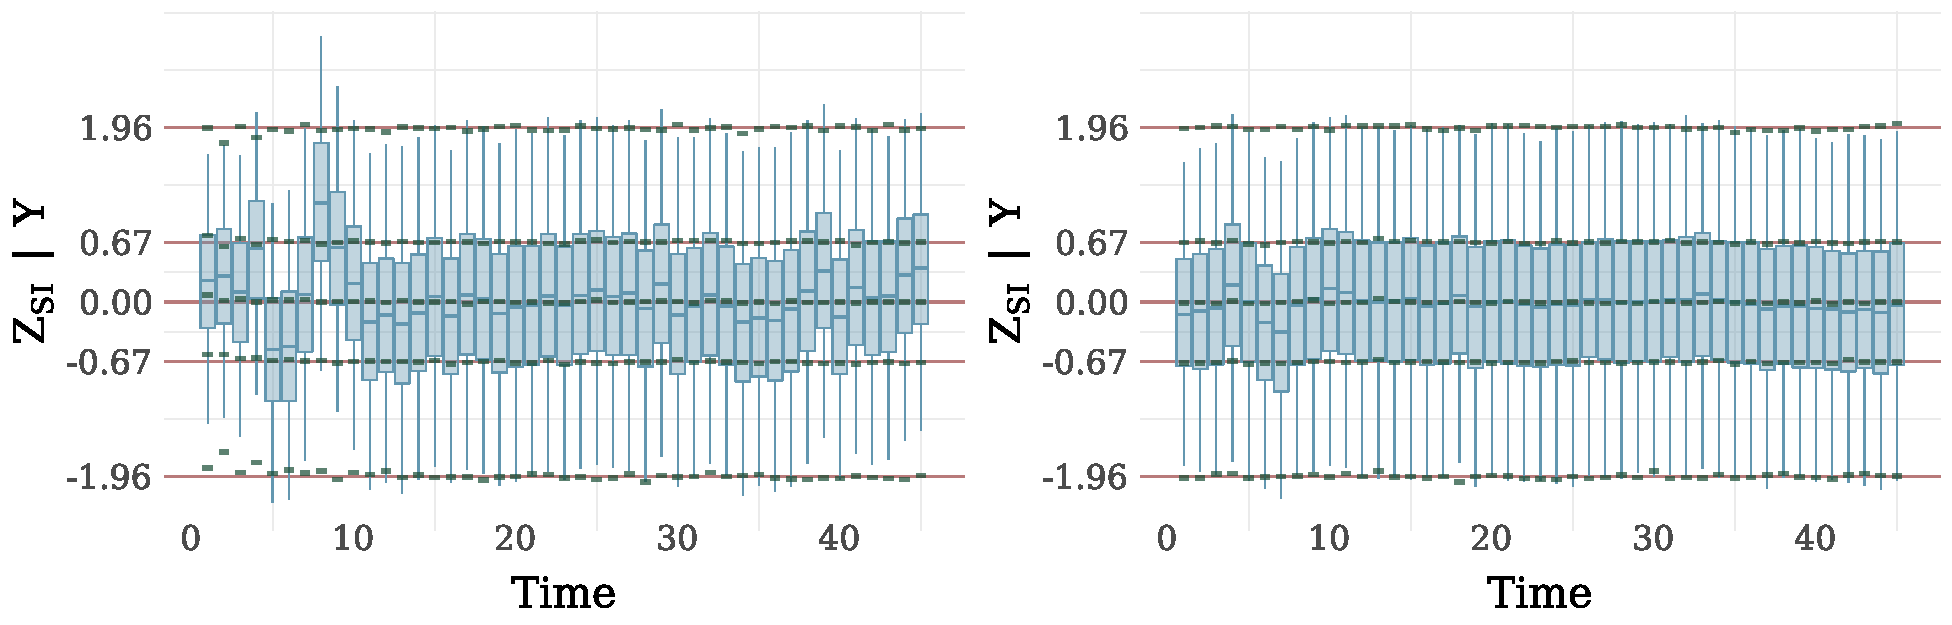
\includegraphics[width=\linewidth]{figures/sir_drawplots}
	\caption[Posterior distributions of LNA draws for an SIR model.]{Posterior distributions of the LNA draws for infections and recoveries in an SIR model (blue boxplots). The lower and upper whisker tips correspond to the $ 2.5^\mr{th} $ and $ 97.5^\mr{th} $ posterior quantiles, the lower and upper hinges to the $ 25^\mr{th} $ and $ 75^\mr{th} $ quantiles, and the middle hash mark to the posterior median. The solid red lines are the theoretical quantiles of the posterior predictive distribution (or equivalently, the prior distribution) of the LNA draws, drawn at the quantiles of a standard normal distribution corresponding to the boxplot quantiles. The green ticks are the estimated quantiles of the posterior predictive distributions of the LNA draws, accounting for boundary conditions on the state space of the latent process and obtained by simulating LNA paths from the posterior predictive distribution. The posterior distributions of LNA draws are shaded according to the level of posterior shrinkage, computed as one minus the ratio of standard deviations of LNA draws in the posterior and prior.}
	\label{fig:sir_drawplots}
\end{figure}

Finally, we can assess whether the model captures the temporal dependencies in the data by computing summary statistics for the observed incidence and posterior predictive incidence. A variety of summary statistics are presented in the supplement of \cite{king2015avoidable}, which are computed and compared for the observed and predicted data. These include the lag 1 autocorrelation (ACF) and the detrended autocorrelations at lags 1, 2, and 3. We will also consider the partial autocorrelation function (PACF) of the log--transformed data. The PACF is a measure of the residual autocorrelation at a particular lag, adjusting for the linear dependencies on the intermediate variables, and is useful in identifying the order of an autoregressive process \cite{brockwell2013time}. We compute the PACF of $ \bYtil = \log(\bY + 0.5) $ at lag $ k $ as 
\begin{align}
\label{eqn:lna_pacf}
\alpha(1)& =  \Cor\left (\bYtil_{(t)}, \bYtil_{(t+1)}\right ), \\
\alpha(k) &= \Cor\left (\bYtil_{(t+k)} - \Proj_{(t,k)}\left (\bYtil_{(t+k)}\right ),\ \bYtil_{(t)} - \Proj_{(t,k)}\left (\bYtil_{(t)}\right )\right ),
\end{align}
where the constant 0.5 is added to stabilize the logarithm for zero counts and $ \Proj_{(t,k)}(\bYtil_{(j)}) $ is the projection of $ \bYtil_{(j)} $ onto the span of $ \bYtil_{(t+1)},\dots,\bY_{(t+k-1)} $ (N.B. this is equivalent to regressing $ \bYtil_{(j)} $ on $ \bYtil_{(t+1)},\dots,\bY_{(t+k-1)} $).  

\begin{figure}[htbp]
	\centering
	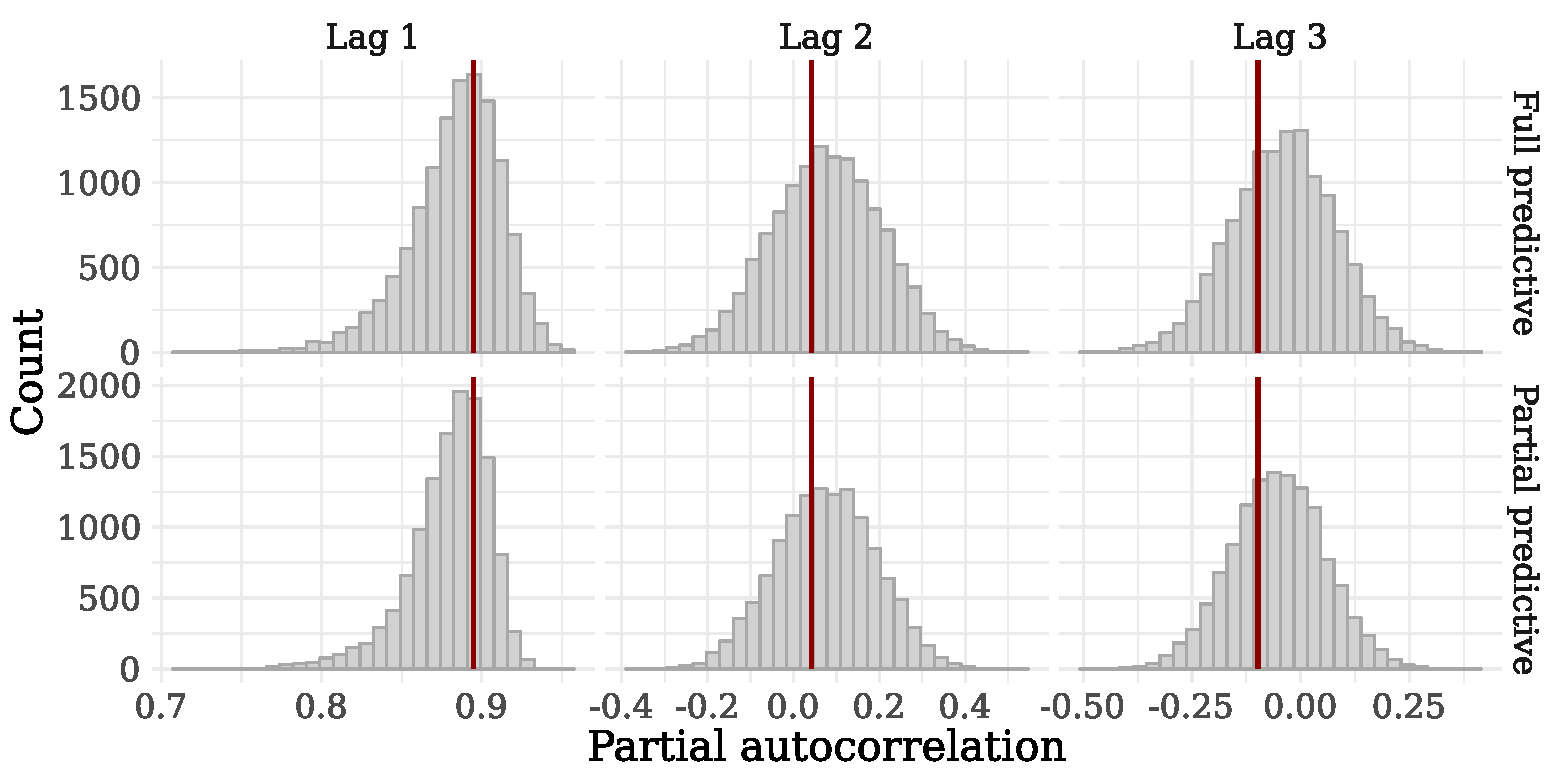
\includegraphics[width=0.9\linewidth]{figures/sir_pacf_plots}
	\caption[Posterior predictive distributions of partial autocorrelations at various lags.]{Distributions of partial autocorrelations at lags 1, 2, and 3 for datasets generated under the full and partial posterior predictive distributions. Vertical red lines are the partial autocorrelations for the observed incidence data at the respective lags.}
	\label{fig:sirpacfplots}
\end{figure}

The distributions of PACFs for the full and partial posterior predictive distributions inform us about whether the temporal structure of the data is reflected in the posterior. A reasonable data generating mechanism should produce data replications that have similar autoregressive structure as the observed data. We might worry about whether the model fails to explain residual dependence in the data if we find that the partial autocorrelation of the data at a particular lag is an outlier with respect to the predictive distribution. This would be particularly concerning if the partial predictive PACF distribution which is conditioned on the data did not reflect the autoregressive structure of the data, especially if it occurs at lag 1, since this would suggest that the emission distribution is misspecified. Figure \ref{fig:sirpacfplots} shows the PACFs generated from the full and partial posterior predictive distributions along with the partial autocorrelations for the observed data. As we expect, since there was no model misspecification, the residual autocorrelation structure in the data appears to be captured by the model.

\subsection{A Stratified SEIR Model for a Simulated Outbreak}
\label{subsec:ebola_synth}

In the next section, we will jointly model the spread of Ebola in Guinea, Liberia, and Sierra Leone during the 2014--2015 outbreak. To do so, we will fit a stratified SEIR model that allows for country specific epidemic dynamics, and transmission between the countries. It should go without saying that this model (or any model), despite being fully stochastic in all aspects of the measurement and epidemic process, is still an overly simplistic abstraction of the outbreak with respect to some obvious and potentially important complexities, e.g., spatial heterogeneity and time varying dynamics. However, it is a good starting point and is non--trivial to fit due to the number of parameters and size of the latent space. Moreover, this simulation will allow us to work with the diagnostics discussed in the previous subsection to develop better intuition for the strengths and weaknesses of the model. 

We simulated data from a three country SEIR model, diagrammed in Figure \ref{fig:stratified_seir_full_diag}, and described briefly below, with additional details in Section \ref{subsec:ebola_synth_setup}. The simulation was designed to crudely reflect the Ebola outbreak in West Africa and allowed for cross--border transmission via the migration of infected individuals between countries. The three countries differed in their true and effective population sizes, times at which transmission commenced, epidemic dynamics, and case detection probabilities. We included a single change--point for the basic reproductive number for Guinea at 33 weeks since the outbreak duration was longest in that country. The change in transmission dynamics coincided roughly with the WHO declaration of a state of emergency in early August 2014 and the closures of country borders with Liberia and Sierra Leone \cite{coltart2017ebola}. The outbreak was simulated from a MJP via Gillespie's direct algorithm \cite{gillespie1976general} using the parameters in Table \ref{tab:ebola_synth_pars} and the rates in Table \ref{tab:ebola_synth_rates_full}. The observed incidence was a negative binomial sample of the true incidence with the case detection probability varying across countries, but with the same value of over--dispersion.

\begin{figure}[htbp]
	\begin{fullpage}
		\resizebox {\linewidth} {!} {
			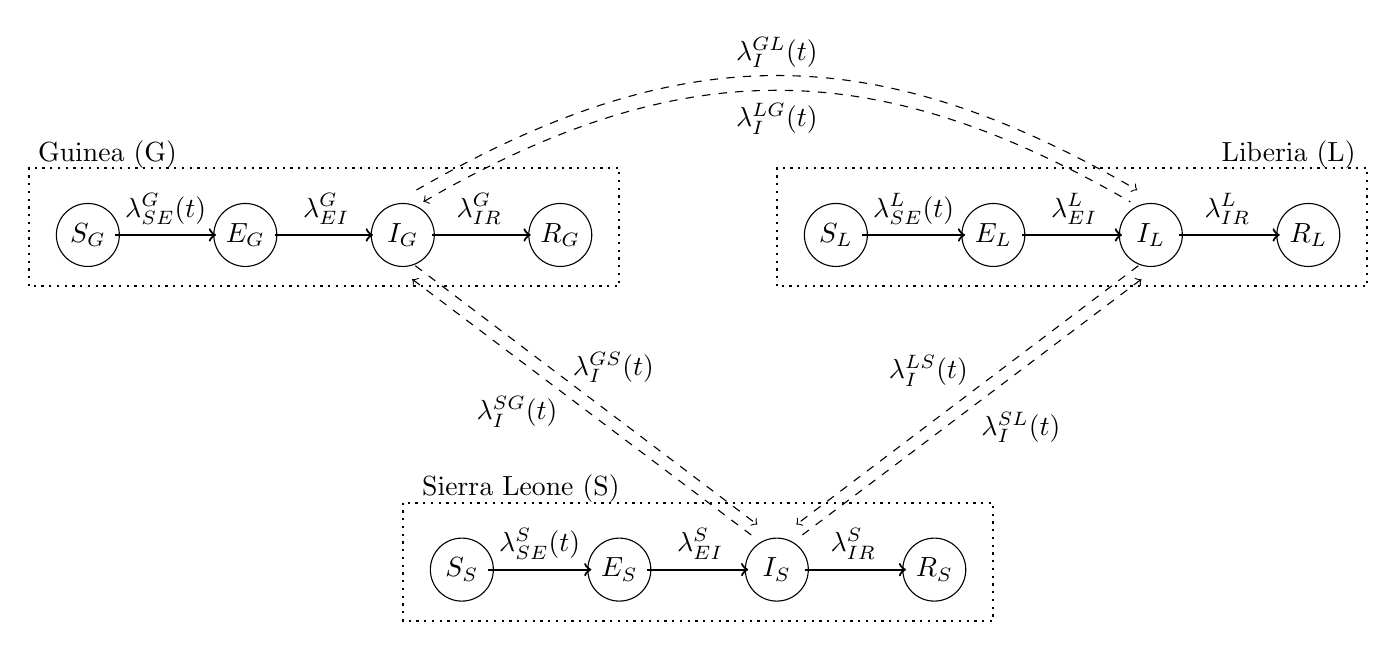
\begin{tikzpicture}
			\draw[thick,dotted] (0,-0.25) rectangle (7.5, 1.25);
			\node at (1, 1) [label=Guinea (G)] {};
			\draw (0.75, 0.4) circle(0.4) node (Sa) {$ S_G $};
			\draw (2.75, 0.4) circle(0.4) node (Ea) {$ E_G $};
			\draw (4.75, 0.4) circle(0.4) node (Ia) {$ I_G $};
			\draw (6.75, 0.4) circle(0.4) node (Ra) {$ R_G $};
			
			\draw[thick,dotted] (9.5,-0.25) rectangle (17, 1.25);
			\node at (16, 1) [label=Liberia (L)] {};	
			\draw (10.25, 0.4) circle(0.4) node (Sb) {$ S_L $};
			\draw (12.25, 0.4) circle(0.4) node (Eb) {$ E_L $};
			\draw (14.25, 0.4) circle(0.4) node (Ib) {$ I_L $};
			\draw (16.25, 0.4) circle(0.4) node (Rb) {$ R_L $};
			
			\draw[thick,dotted] (4.75,-3) rectangle (12.25, -4.5);
			\node at (6.25, -3.25) [label=Sierra Leone (S)] {};	
			\draw (5.5, -3.85) circle(0.4) node (Sc) {$ S_S $};
			\draw (7.5, -3.85) circle(0.4) node (Ec) {$ E_S $};
			\draw (9.5, -3.85) circle(0.4) node (Ic) {$ I_S $};
			\draw (11.5, -3.85) circle(0.4) node (Rc) {$ R_S $};
			
			\draw [thick,->] (Sa) -- (Ea) node[midway,above] {$ \lambda_{SE}^G(t) $};
			\draw [thick,->,shorten >=.6mm] (Ea) -- (Ia) node[midway,above] {$ \lambda_{EI}^G $};
			\draw [thick,->,shorten <=.5mm] (Ia) -- (Ra) node[midway,above] {$ \lambda_{IR}^G $};
			
			\draw [thick,->] (Sb) -- (Eb) node[midway,above] {$ \lambda_{SE}^L(t) $};
			\draw [thick,->,shorten >=.6mm] (Eb) -- (Ib) node[midway,above] {$ \lambda_{EI}^L $};
			\draw [thick,->,shorten <=.5mm] (Ib) -- (Rb) node[midway,above] {$ \lambda_{IR}^L $};
			
			\draw [thick,->] (Sc) -- (Ec) node[midway,above] {$ \lambda_{SE}^S(t) $};
			\draw [thick,->,shorten >=.6mm] (Ec) -- (Ic) node[midway,above] {$ \lambda_{EI}^S $};
			\draw [thick,->,shorten <=.5mm] (Ic) -- (Rc) node[midway,above] {$ \lambda_{IR}^S $};
			
			\path [dashed, <-] ([yshift=-0.5mm,xshift=-2mm]Ia.south) edge [shorten >= 2mm, shorten <= 4mm] node [above,xshift=4.5mm,yshift=1.5mm] {$ \lambda_I^{GS}(t) $} ([xshift=-1mm]Ic.north);
			\path [dashed, ->] (Ia.south) edge [shorten >= 5mm, shorten <= 2mm] node [below,xshift=-10mm,yshift=2mm] {$ \lambda_I^{SG}(t) $} ([xshift=1.5mm]Ic.north);
			
			\path [dashed, <-] ([yshift=-0.5mm,xshift=2mm]Ib.south) edge [shorten >= 2mm, shorten <= 4mm] node[above,yshift=1mm,xshift=-6mm] {$ \lambda_I^{LS}(t) $} ([xshift=1mm]Ic.north);
			\path [dashed, ->] (Ib.south) edge [shorten >= 5mm, shorten <= 2mm] node[below,xshift=8mm] {$ \lambda_I^{SL}(t) $} ([xshift=-1.5mm]Ic.north);
			
			\path [dashed, <-] ([]Ia.north) edge [shorten >= 3mm, shorten <= 3mm, bend left, looseness=1.1] node [below] {$ \lambda_I^{LG}(t) $} ([]Ib.north);
			\path [dashed, ->] ([]Ia.north) edge [shorten >= 2mm, shorten <= 2mm, bend left, looseness=1.1,yshift=2mm] node [above] {$ \lambda_I^{GL}(t) $} ([]Ib.north);	
			\end{tikzpicture}
		}
		\caption[Diagram of a stratified SEIR model with country specific outbreak dynamics and cross--country virtual transmission.]{Diagram of state transitions for a stratified SEIR model fit to a simulated Ebola outbreak in Guinea, Liberia, and Sierra Leone. Dashed boxes denote countries, nodes in circles denote the model compartments: susceptible (S), exposed (E), infectious (I), recovered (R). Compartments  are subscripted with country indicators. Solid lines with arrows indicate stochastic transitions between model compartments, which occur continuously in time. Dashed lines indicate virtual migrations, where infected individuals in one country contribute to the force of infection in another country but do not migrate. Rates at which individuals transition between compartments are denoted by $ \lambda $ and are subscripted by compartments and superscripted by countries, e.g., $ \lambda_{SE}^L $ is the rate at which susceptible individuals become exposed in Liberia, $ \lambda_I^{SG} $ is the rate at which an infected individual in Sierra Leone migrates to Guinea. The rate at which susceptibles in Guinea become infected is time varying with one change--point at 33 weeks. Transmission in Liberia and Sierra Leone commenced at 10 and 19 weeks, respectively. Full expressions for the rates are given in Table \ref{tab:ebola_synth_rates_approx}.}
		\label{fig:stratified_seir_approx_diag}
	\end{fullpage}
\end{figure}

We fit a stratified SEIR model to the simulated data that was largely the same as the model used in simulating the data, except with respect to migration of infected individuals from one country to another. In this example, as we would expect for the real--world Ebola outbreak, transmission to susceptibles was largely driven by contacts with natively infected individuals within the same country. Here, we approximate the contribution of cross--border transmission to the local force of infection by replacing migrations of infected individuals with virtual migrations that modify the effective number of infected individuals in a country. Hence, we replace the rates at which individuals become infected in country A and import infections from countries B and C,
\begin{align}
\label{eqn:foi_migration}
\lambda_{SE}^A(t) &= \beta_A S_A I_A\ind{t\geq t_{0}^A}, \\
\lambda_I^{BA}(t) &= \alpha_BI_B\ind{t\geq t_{0}^A}\ind{t\geq t_{0}^B},\ \hspace{0.1in} \lambda_I^{CA}(t) = \alpha_CI_C\ind{t\geq t_{0}^A}\ind{t\geq t_{0}^C},
\end{align}
with the approximate rates,
\begin{align}
\label{eqn:foi_virtual}
\lambda_{SE}^A &= \beta_AS_A\left (I_A + \alpha_{BA}I_B\ind{t\geq t_{0}^B} + \alpha_{CA}I_C\ind{t\geq t_{0}^C}\right )\ind{t\geq t_{0}^A}\\
\lambda_I^{BA} &= \lambda_I^{CA} = 0,
\end{align}
where $ \beta_A $ is the per--contact rate of infection in country A, $ \alpha $ are parameters are the rates of real or virtual migration of infected individuals from countries B and C, $ t_0 $ is the time at which transmission was assumed to commence in each country. We note that the models are approximately equivalent to the extent that the infectious period durations in each country are similar and that the contribution to the local force of infection from other countries is relatively minimal. The upside is that the quantities, $ \alpha_{BA}I_B $ and $ \alpha_{CA}I_C$, are interpretable as the effective number of infected individuals from countries B and C with whom susceptibles in country A come into contact. The approximate model is also more computationally tractable since we have fewer ODEs to solve in the LNA approximation and fewer boundary conditions on the LNA state space. Finally, the approximate model is arguably more appropriate from the standpoint of the LNA approximation since the rates of infectious migration events are low. The full model with explicit migration was fit as a supplementary analysis and yielded generally similar results (see Table \ref{tab:ebola_synth_ests}), other than cross--border transmission parameters, which were poorly estimated.  

Before proceeding, we pause to note that the effective population size and case detection probability and effective population size are only weakly identifiable in this model. Rather, the mean case detection rate, $ \rho N_{eff} $, is estimable because of its relationship to the true and observed outbreak sizes. In practice, we require prior information about either $ \rho $ or $ N_{eff} $ in order to estimate the parameters separately. This is discussed further in Section \ref{sec:effpop_identifiability}. 

We fit the model using a combination of weakly informative priors for the effective reproductive numbers, informative priors for the latent period durations, infectious period durations, and cross--border transmission parameters, and diffuse priors for the measurement process parameters and effective population sizes (Table \ref{tab:ebola_synth_pars}). The 95\% credible intervals contained the true values (Figure \ref{fig:ebola_synth_posts}) for all parameters, or identifiable functions as for the case detection rate. We essentially recover the priors for parameters that were assigned informative priors. 

Although the latent epidemic process is not identifiable in this model, we recover, for the most part, the mean incidence we would have expected to observe if the true incidence were known (Figure \ref{fig:ebola_synth_diags}). The partial posterior predictive distributions capture the observed incidence curves, suggesting that the emission distribution adequately described the sampling process for the observed incidence, conditional on the latent incidence being distributed according to its posterior. The full posterior predictive distributions for Guinea and Sierra Leone suggest that the model may be a reasonable data generating mechanism for the outbreaks in those countries. However, the full posterior predictive distribution for Liberia predicts slower dynamics than were actually observed, which is reflective of an estimated effective reproductive number for Liberia that was somewhat lower than the true value. There is also some residual autocorrelation in the log transformed data for Liberia that was not well captured in the posterior predictive distributions (Figure \ref{fig:ebola_synth_pacfs}), unlike Guinea and Sierra Leone. Finally, the posterior distributions of the LNA draws suggest that the LNA approximation might not fully account for the uncertainty in the latent epidemic process, particularly in Guinea and Liberia. This is expected since the effective population sizes were not particularly large and the data included incidence from the beginning and end of the outbreak, when the relative stochasticity was large. The posterior LNA draws for Guinea, which had the smallest effective population size, are more variable than we would expect under the LNA prior. The posterior and posterior predictive draws for Liberia exhibit systematic deviations from normality during the periods when transmission commenced and tailed off.

\begin{sidewaysfigure}[htbp]
	\begin{fullpage}
		\centering
		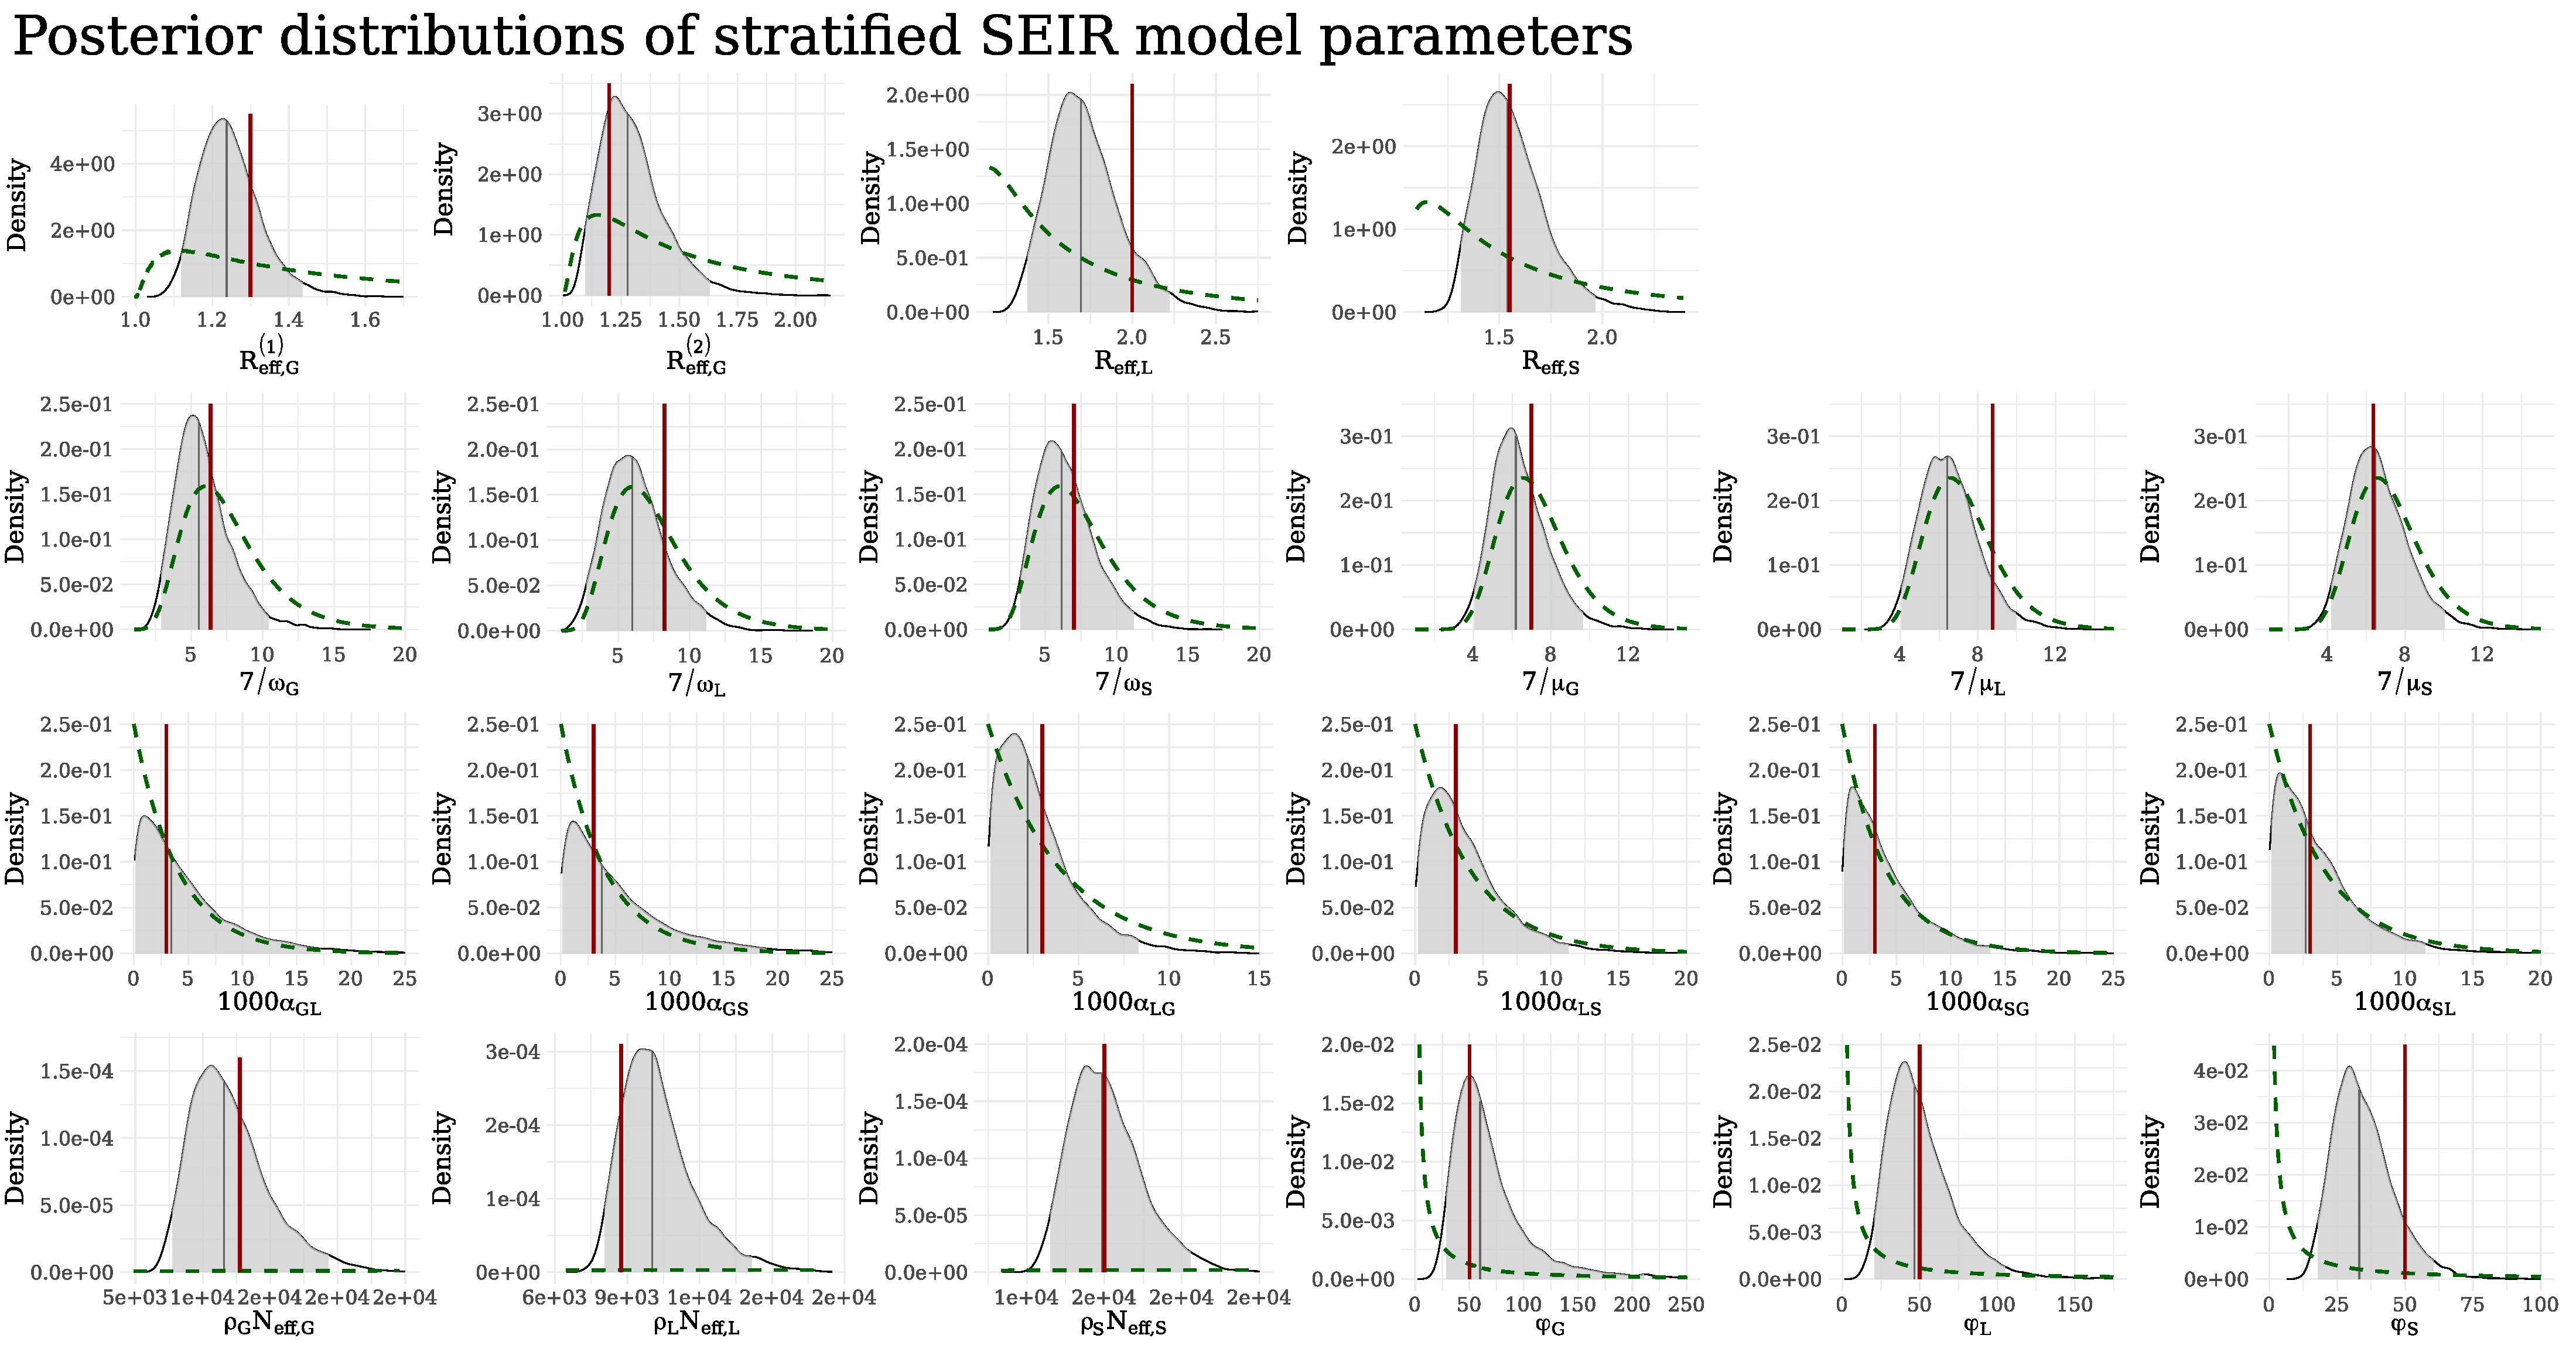
\includegraphics[width=\linewidth]{figures/ebola_synth_posts}
		\caption[Posterior distributions of stratified SEIR model parameters for a simulated Ebola outbreak in three countries.]{Posterior distributions of parameters of a stratified SEIR model for a simulated Ebola outbreak in three countries. We show posterior medians (solid gray lines), 95\% Bayesian credible intervals (light gray areas under the posterior densities), prior densities (induced priors for the reporting rate and latent period durations) over the posterior ranges (dashed green curves), and true parameter values (solid red lines). $ R_{eff} = \beta N_{eff}/\mu $ is the effective reproductive number, where $ \beta $ is the per--contact infection rate, $ N_{eff} $ is the effective population size, and $ \mu $ is the recovery rate. The latent and infectious period durations, $ 7/\omega $ and $ 7/\mu $, respectively, are given in days. The effective number of cross--border infectious contacts in country $ B $ per 1000 infected individuals in country $ A $ is $ 1000\alpha_{AB} $. The effective reporting rate is $ \rho N_{eff} $, and $ \phi $ is the negative binomial over--dispersion parameter. Subscripts indicate countries.}
		\label{fig:ebola_synth_posts}
	\end{fullpage}
\end{sidewaysfigure}

\begin{figure}[htbp]
	\begin{fullpage}
		\centering
		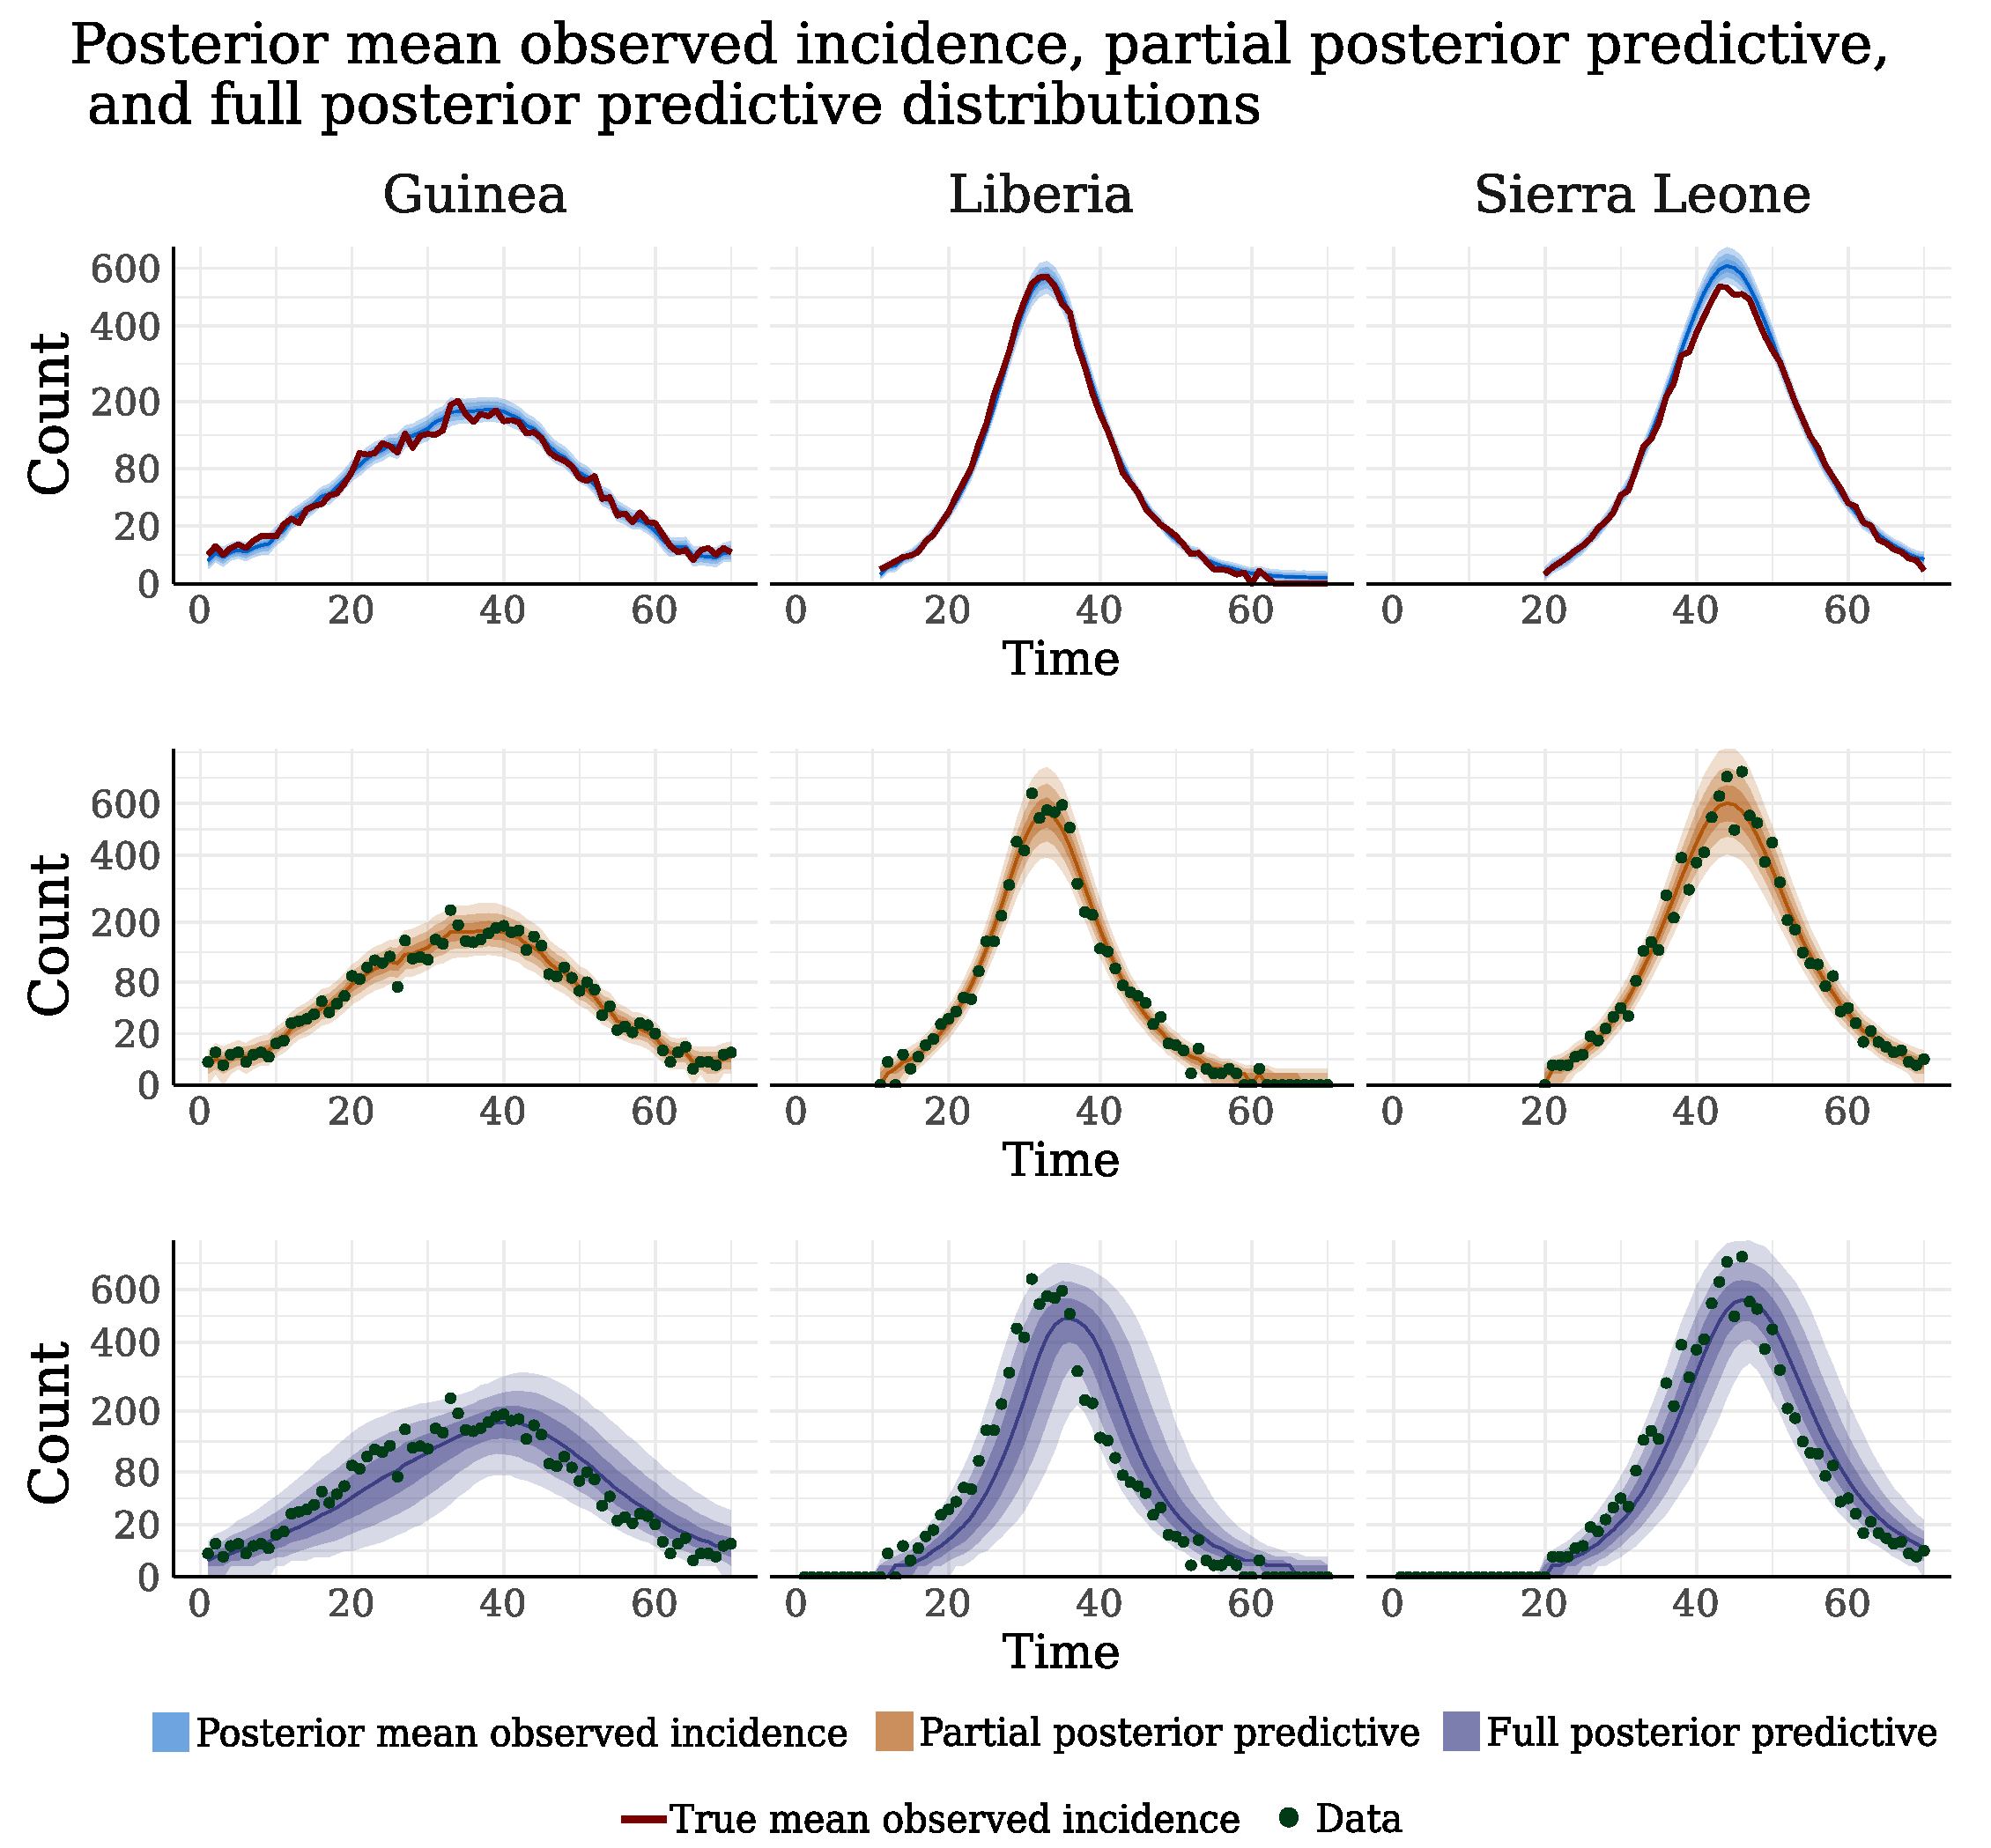
\includegraphics[width=\linewidth]{figures/ebola_synth_diag_plots}
		\caption[Posterior mean observed incidence, partial posterior predictive, and full posterior distributions for a stratified SEIR model fit to a simulated Ebola outbreak.]{From top to bottom, the posterior mean observed incidence, partial posterior predictive, and full posterior predictive distributions. The solid red line is the incidence we would expect to observe if we knew the true incidence. Green points correspond to the observed incidence. The shaded bands, in order of lightest to darkest, correspond to pointwise posterior 95\%, 80\%, and 50\% credible intervals, with the pointwise posterior median given by the corresponding colored solid line.}
		\label{fig:ebola_synth_diags}
	\end{fullpage}
\end{figure}

\begin{figure}[htbp]
	\begin{fullpage}
		\centering
		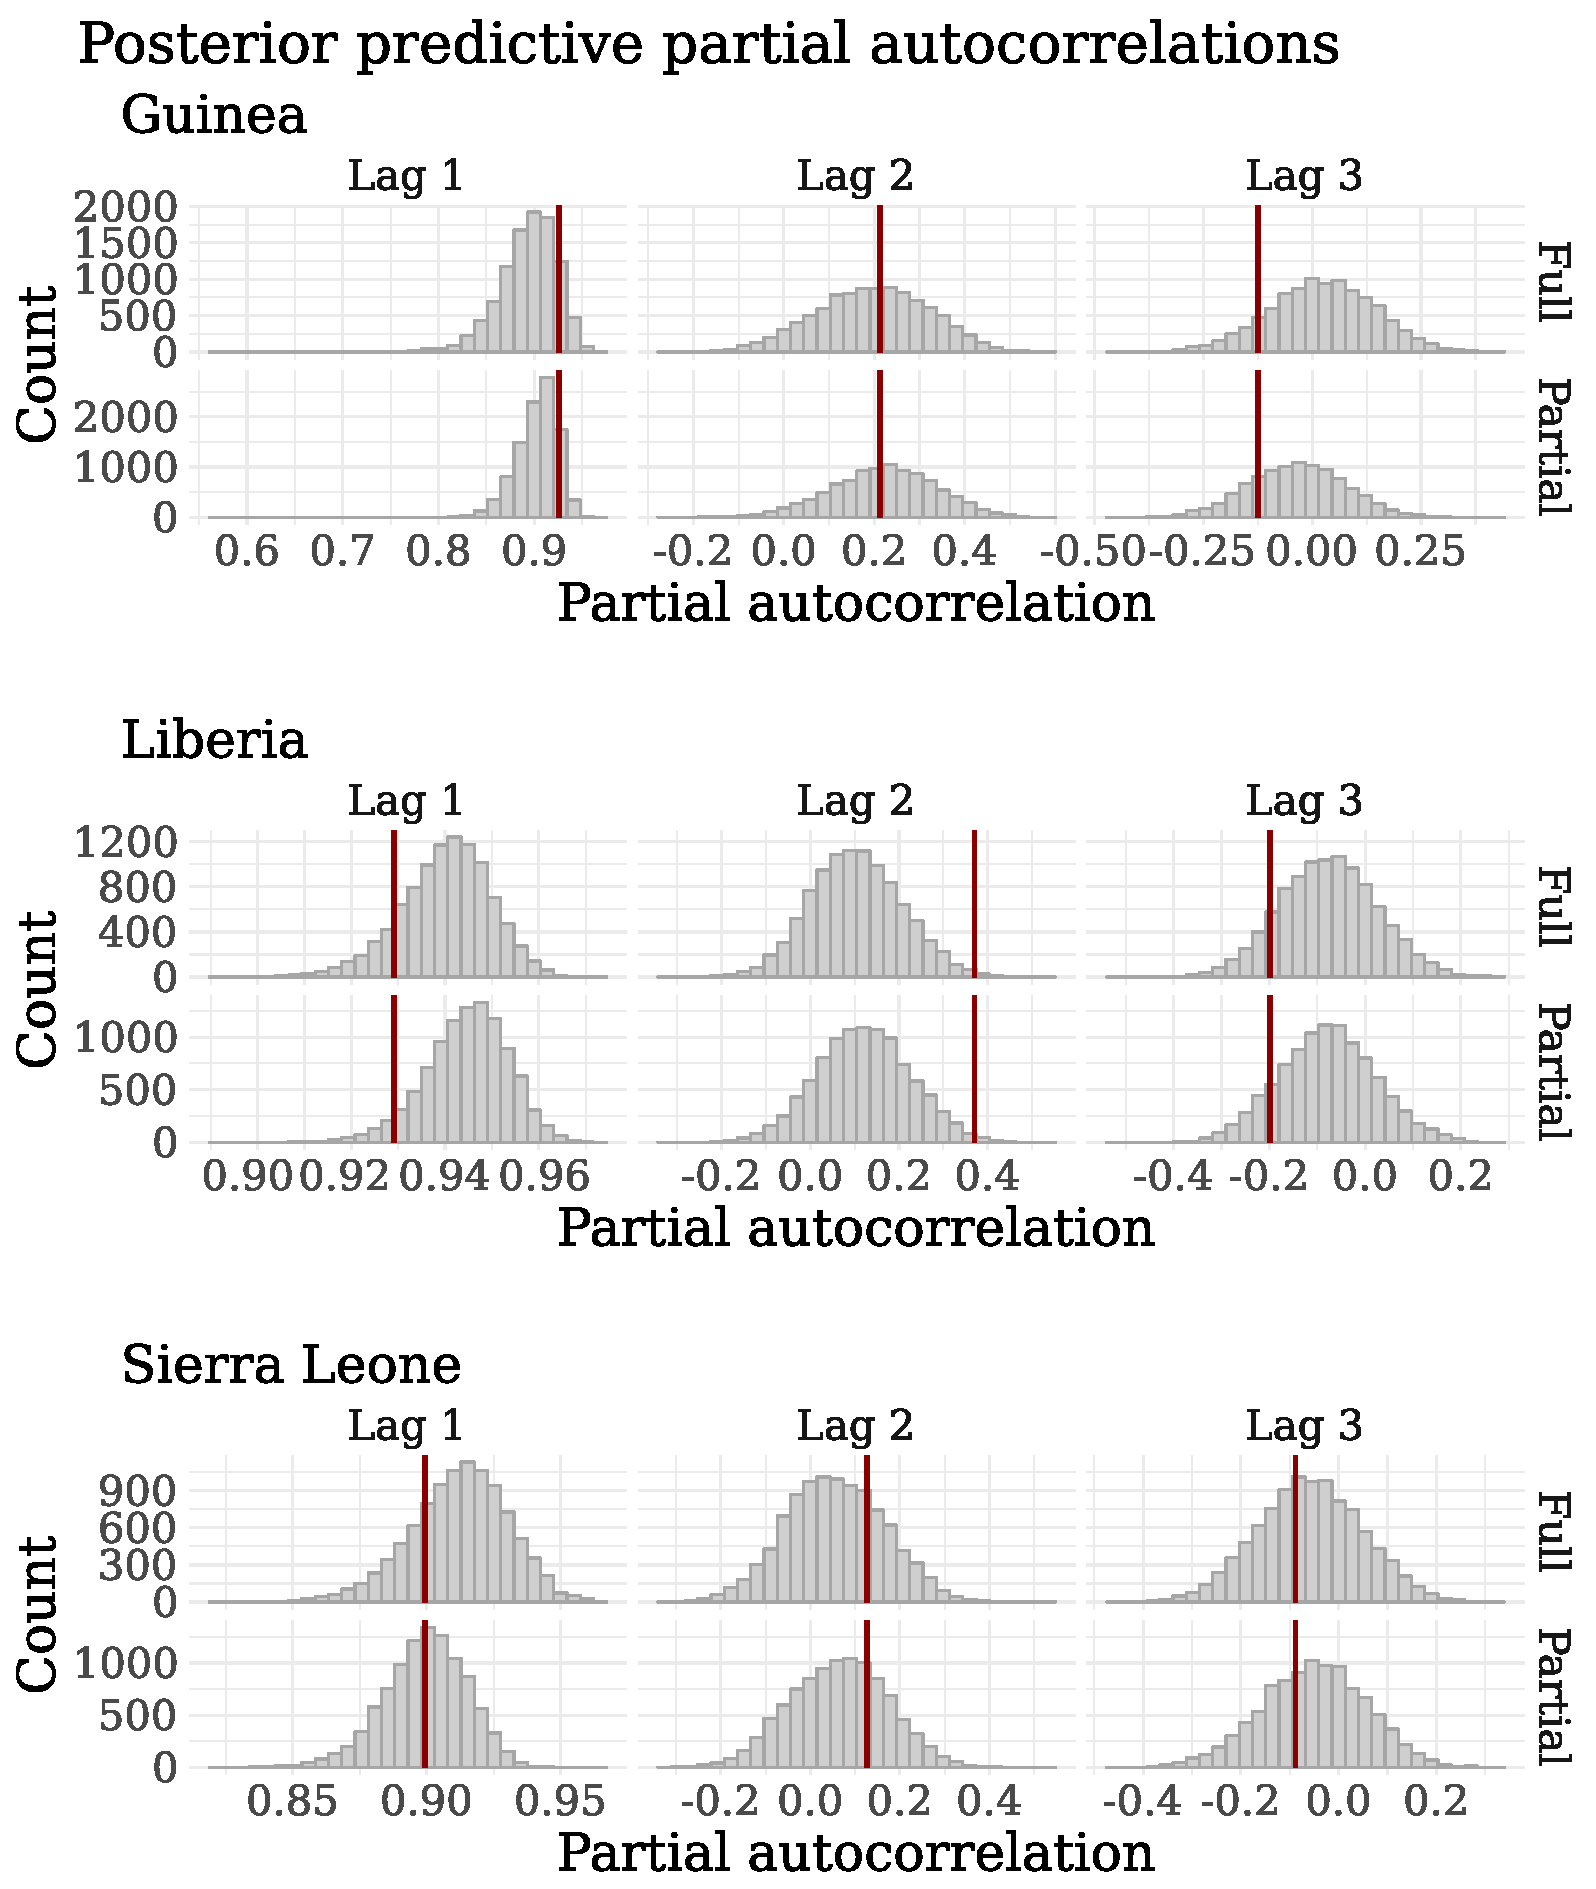
\includegraphics[width=0.8\linewidth]{figures/ebola_synth_pacfs}
			\caption[Posterior predictive distributions of partial autocorrelations for a stratified SEIR model fit to a simulated Ebola outbreak.]{Distributions of partial autocorrelations at lags 1, 2, and 3 for datasets generated under the full and partial posterior predictive distributions. Vertical red lines are the partial autocorrelations for the observed incidence data at the respective lags.}
		\label{fig:ebola_synth_pacfs}
	\end{fullpage}
\end{figure}

\begin{sidewaysfigure}[htbp]
	\begin{fullpage}
		\centering
		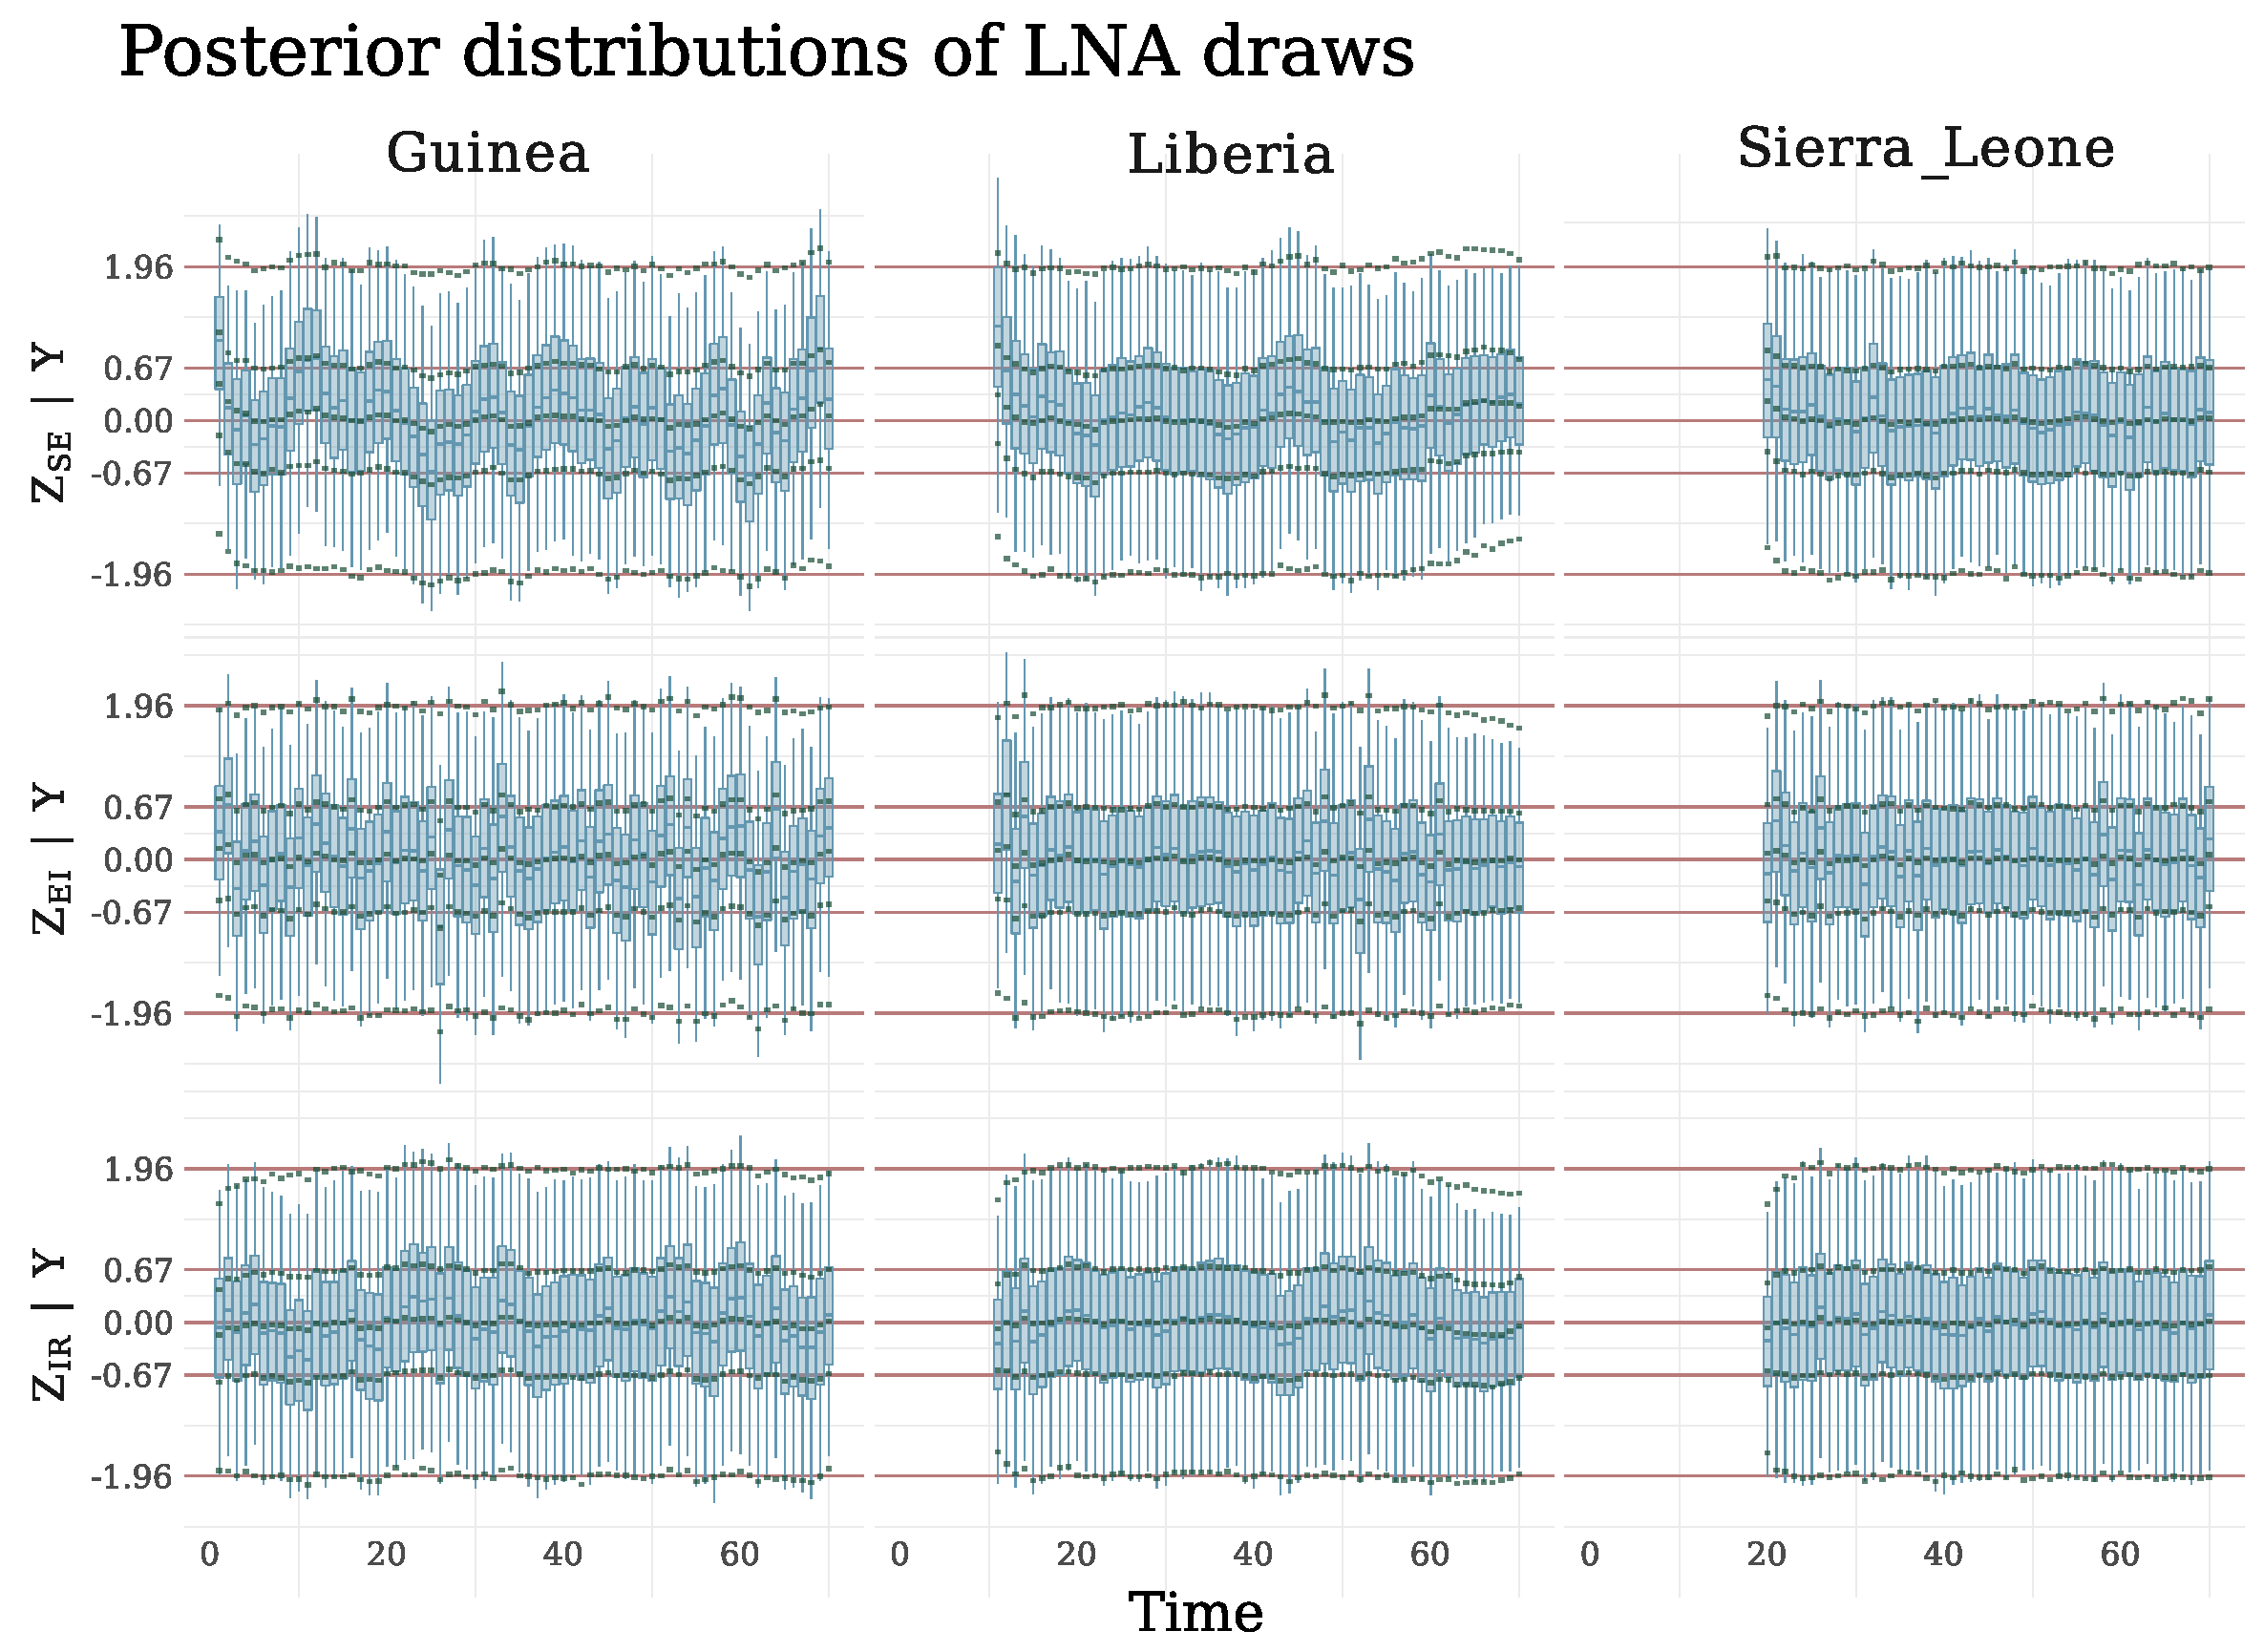
\includegraphics[width=\linewidth]{figures/ebola_synth_drawplots}
		\caption[Posterior distributions of LNA draws for a stratified SEIR model fit to a simulated Ebola outbreak.]{Posterior distributions of the LNA draws for exposures, infections, and recoveries (blue boxplots) in a stratified SEIR model fit to a simulated Ebola outbreak in Guinea, Liberia, and Sierra Leone. The lower and upper whisker tips correspond to the $ 2.5^\mr{th} $ and $ 97.5^\mr{th} $ posterior quantiles, the lower and upper hinges to the $ 25^\mr{th} $ and $ 75^\mr{th} $ quantiles, and the middle hash mark to the posterior median. The solid red lines are the theoretical quantiles of the posterior predictive distribution (or equivalently, the prior distribution) of the LNA draws, drawn at the quantiles of a standard normal distribution corresponding to the boxplot quantiles. The green ticks are the estimated quantiles of the posterior predictive distributions of the LNA draws, accounting for boundary conditions on the state space of the latent process and obtained by simulating LNA paths from the posterior predictive distribution.  The posterior distributions of LNA draws are shaded according to the level of posterior shrinkage, computed as one minus the ratio of standard deviations of LNA draws in the posterior and prior.}
		\label{fig:ebola_synth_drawplots}
	\end{fullpage}
\end{sidewaysfigure}

\newpage
\section{Application: Modeling the Spread of Ebola}
\label{sec:lna_ebola}
Starting in December 2013, the West African countries of Guinea, Liberia, and Sierra Leone experienced an outbreak of Ebola that was unprecedented in its size and duration compared to previous Ebola outbreaks. The first cases were thought to have occurred in December 2013 in the Gu\'{e}d\'{e}ckou prefecture in Guinea, while the first cases in Liberia and Sierra Leone were detected on March 30 and June 12, 2014, respectively. By March 2016, a total of 28,646 suspected, probable, and confirmed cases had been reported along with 11,323 deaths \cite{who2016situation}. The outbreak was exacerbated by a number of factors including insufficient outbreak response infrastructure, highly transient populations, and failures to engage with communities early on in the outbreak to implement infection prevention and control measures \cite{coltart2017ebola,dudas2017virus}. 

Mathematical models were key tools in informing decisions about resource allocation and interventions throughout the outbreak \cite{coltart2017ebola}. A 2015 literature review of 66 modeling studies comprising 125 models for the population--level spread of the outbreak found that modelers typically relied on pre--existing publicly available epidemiological data, which most often consisted of aggregate count data such as weekly incidence counts published by the WHO or national ministries of health \cite{chretien2015mathematical}. Modelers working with incidence data were most often interested in describing the transmission dynamics, particularly the basic reproductive number. Other objectives included forecasting the possible time--evolution of the outbreak, and constructing models to assess the effects of various interventions on the transmission dynamics. Although modeling teams working with publicly available data were not always involved in the policy--making process, the importance of developing outbreak models using real--world data, during what for those teams would be "peace time", has been emphasized as a critical exercise in preparing for future outbreaks \cite{viboud2018rapidd}.

We now apply our methods to model the spread of Ebola in Guinea, Liberia, and Sierra Leone during the 2013--2016 Ebola outbreak. Our objective will be to describe the transmission dynamics of the outbreak, and in particular to estimate the basic reproductive number. The data, shown in Figure \ref{fig:eboladat}, consist of national case counts from the World Health Organization patient database consisting of weekly confirmed and probable Ebola cases \cite{who2016eboladat}. Individuals were classified as suspected cases if they presented with Ebola--like symptoms and had contact with a suspected, probable, or confirmed case of a dead or sick animal. Probable cases consisted of suspected cases who were evaluated by a clinician, or who had died but were epidemiologically linked to confirmed cases. A confirmed case was defined as a suspected or probable case testing positive for Ebola virus RNA or IgM Ebola antibodies \cite{coltart2017ebola}. For the purpose of this analysis, we will lump together confirmed and probable cases.

\begin{figure}[htbp]
	\centering
	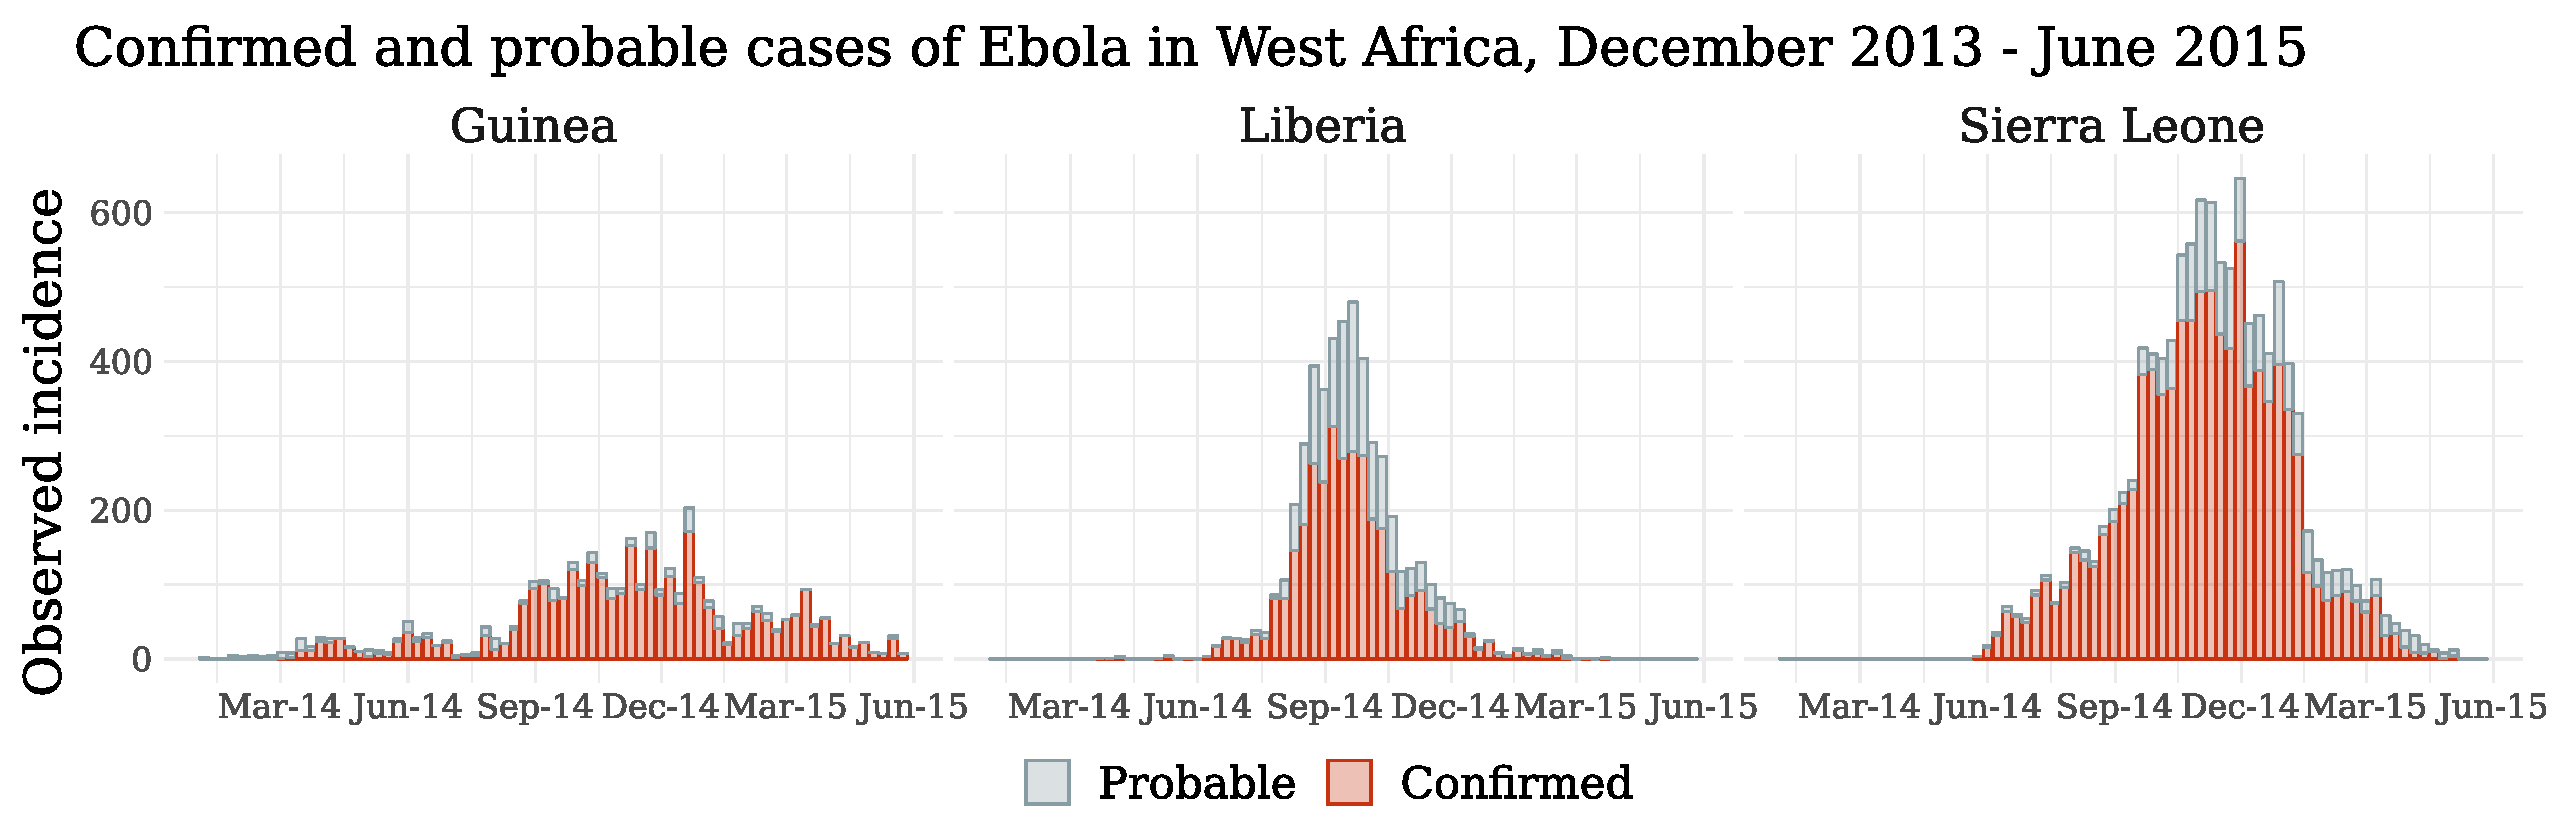
\includegraphics[width=\linewidth]{figures/ebola_dat}
	\caption{Weekly incidence of confirmed and probable cases of Ebola in Guinea, Liberia, and Sierra Leone.}
	\label{fig:eboladat}
\end{figure}

There are several reasons to suspect that the true incidence is significantly under--counted in the dataset. First, suspected cases accounted for sizable fractions of the total case counts, particularly in the case of Liberia, but were not available as part of this dataset (see Table \ref{tab:ebola_descriptives}). Furthermore, analyses based on phylogenetic data \cite{scarpino2014epidemiological} and case fatality ratios \cite{atkins2015under,garske2017heterogeneities} suggest that many cases may have gone undetected, particularly in the early stages, and during the peak, of the outbreak when health systems were overwhelmed. 

\begin{table}[htbp]
	\caption[Ebola incidence by country and case type]{WHO cumulative Ebola incidence by country and case type through May 24, 2015 \cite{who2016eboladat}. Suspected cases were computed as the difference between the official CDC total \cite{cdc2016eboladat}, which included all three case types, and the WHO confirmed plus probable cases.}
	\label{tab:ebola_descriptives}
	\small
	\centering
	\begin{tabular}{lcccc}	
		\hline	
		& \textbf{Guinea} & \textbf{Liberia} & \textbf{Sierra Leone} & \textbf{Total} \\\hline
		\textbf{Confirmed}$ ^1 $ & 3,210 & 3,342 & 9,494 & 16,044\\ 
		\textbf{Probable}$ ^1 $ & 419 & 1,652 & 1,823 & 3,894 \\
		\textbf{Suspected$ ^2 $} & 12 & 5,672 & 1,389 & 7,073 \\
		\hline
		\textbf{Total} & 3,641 & 10,666 & 12,706 & 27,013 \\
		\hline
		\multicolumn{5}{l}{\scriptsize $ ^1 $ Dataset used in the current analysis, cases through 05--24--2015.}\\
		\multicolumn{5}{l}{\scriptsize $ ^2 $ Not available as part of the dataset for this analysis.}\\
	\end{tabular} 
\end{table}

\subsection{Country--Specific and Joint Models for the Spread of Ebola in West Africa}
\label{subsec:ebola_models}

\subsubsection{Country--Specific Models}
\label{subsubsec:ebola_single_models}
A typical first step in learning about the overall outbreak dynamics is to separately model the incidence data from each country. This is less challenging than fitting a joint model that incorporates cross--border transmission since each model will have fewer parameters and a smaller latent state space. Furthermore, as we discuss in Section \ref{sec:est_scale_discussion}, iterating through simplified models is helpful in identifying parameterizations that simplify the posterior geometry and that we will use in fitting the more complicated joint model discussed in the next section. 

\begin{figure}[htbp]
	\begin{fullpage}
		\resizebox {\linewidth} {!} {
			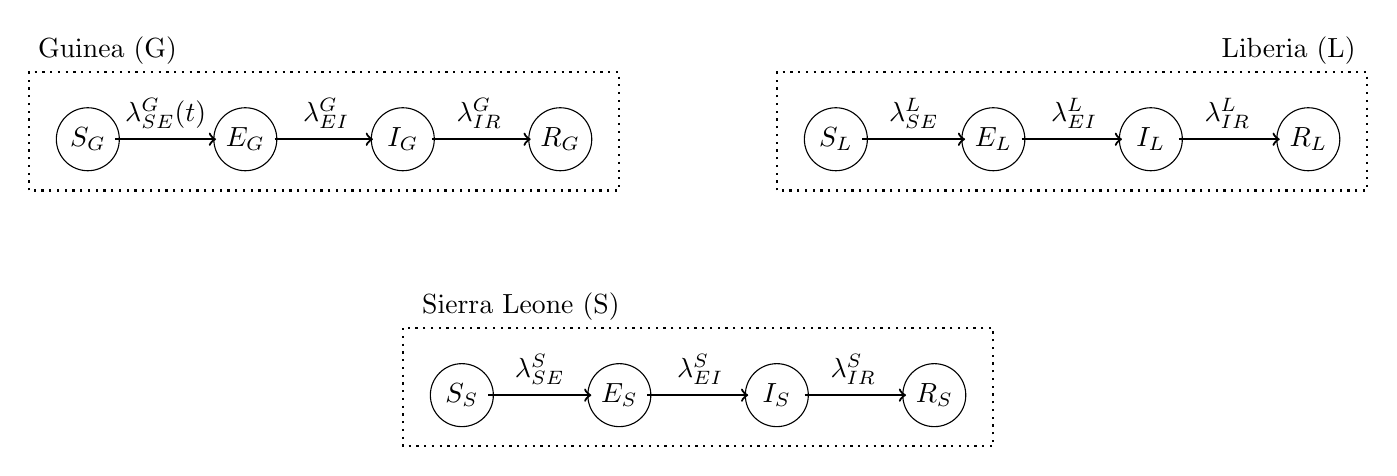
\begin{tikzpicture}
			\draw[thick,dotted] (0,-0.25) rectangle (7.5, 1.25);
			\node at (1, 1.1) [label=Guinea (G)] {};
			\draw (0.75, 0.4) circle(0.4) node (Sa) {$ S_G $};
			\draw (2.75, 0.4) circle(0.4) node (Ea) {$ E_G $};
			\draw (4.75, 0.4) circle(0.4) node (Ia) {$ I_G $};
			\draw (6.75, 0.4) circle(0.4) node (Ra) {$ R_G $};
			
			\draw[thick,dotted] (9.5,-0.25) rectangle (17, 1.25);
			\node at (16, 1.1) [label=Liberia (L)] {};	
			\draw (10.25, 0.4) circle(0.4) node (Sb) {$ S_L $};
			\draw (12.25, 0.4) circle(0.4) node (Eb) {$ E_L $};
			\draw (14.25, 0.4) circle(0.4) node (Ib) {$ I_L $};
			\draw (16.25, 0.4) circle(0.4) node (Rb) {$ R_L $};
			
			\draw[thick,dotted] (4.75,-2) rectangle (12.25, -3.5);
			\node at (6.25, -2.15) [label=Sierra Leone (S)] {};	
			\draw (5.5, -2.85) circle(0.4) node (Sc) {$ S_S $};
			\draw (7.5, -2.85) circle(0.4) node (Ec) {$ E_S $};
			\draw (9.5, -2.85) circle(0.4) node (Ic) {$ I_S $};
			\draw (11.5, -2.85) circle(0.4) node (Rc) {$ R_S $};
			
			\draw [thick,->] (Sa) -- (Ea) node[midway,above] {$ \lambda_{SE}^G(t) $};
			\draw [thick,->,shorten >=.6mm] (Ea) -- (Ia) node[midway,above] {$ \lambda_{EI}^G $};
			\draw [thick,->,shorten <=.5mm] (Ia) -- (Ra) node[midway,above] {$ \lambda_{IR}^G $};
			
			\draw [thick,->] (Sb) -- (Eb) node[midway,above] {$ \lambda_{SE}^L $};
			\draw [thick,->,shorten >=.6mm] (Eb) -- (Ib) node[midway,above] {$ \lambda_{EI}^L $};
			\draw [thick,->,shorten <=.5mm] (Ib) -- (Rb) node[midway,above] {$ \lambda_{IR}^L $};
			
			\draw [thick,->] (Sc) -- (Ec) node[midway,above] {$ \lambda_{SE}^S $};
			\draw [thick,->,shorten >=.6mm] (Ec) -- (Ic) node[midway,above] {$ \lambda_{EI}^S $};
			\draw [thick,->,shorten <=.5mm] (Ic) -- (Rc) node[midway,above] {$ \lambda_{IR}^S $};
			\end{tikzpicture}
		}
		\caption[Diagram of single country SEIR models for the Ebola outbreak in West Africa.]{Diagram of state transitions for SEIR models fit to Ebola incidence data from Guinea, Liberia, and Sierra Leone. Dashed boxes denote countries, nodes in circles denote the model compartments: susceptible (S), exposed (E), infectious (I), recovered (R). Compartments  are subscripted with country indicators. The number of susceptible individuals is equal to the effective population size, estimated as a parameter in the model, minus the numbers of exposed, infected, and recovered individuals. Solid lines with arrows indicate stochastic transitions between model compartments, which occur continuously in time. Rates at which individuals transition between compartments are denoted by $ \lambda $ and are subscripted by compartments and superscripted by countries, e.g., $ \lambda_{SE}^L $ is the rate at which susceptible individuals become exposed in Liberia. The rate at which susceptibles in Guinea become infected is time varying with one change--point at 33 weeks. Transmission in Liberia and Sierra Leone commenced at 10 and 19 weeks, respectively. Full expressions for the rates are given in Table \ref{tab:ebola_rates_single}.}
		\label{fig:ebola_single_diag}
	\end{fullpage}
\end{figure}

We fit separate SEIR models, diagrammed in Figure \ref{fig:ebola_single_diag}, to the incidence data from each country using both the LNA and ODE approximations. Transmission was modeled in Liberia beginning March 2, 2014, and in Sierra Leone from May 4, 2014, corresponding to three weeks prior to the first confirmed or probable cases in those countries. Phylogeographic models fit to viral sequence data collected during the outbreak suggested that Guinea experienced re--importation of Ebola throughout the outbreak from Liberia and Sierra Leone \cite{dudas2017virus}. Therefore, we included a single change--point for the effective reproductive number for Guinea to account for possible changes in the outbreak dynamics. The change--point was set to August 10, 2014, two days after the WHO declared an international state of emergency, and one day after borders were closed with Sierra Leone and Liberia \cite{coltart2017ebola}. The force of infection in each country included a constant term for infectious contact from outside the population. To account for the small scale of each outbreak relative to the population size in the country, we estimate the effective population size as a parameter in the model. The number of susceptible individuals is then equal to the effective population size, minus the numbers of exposed, infected, and recovered individuals. The implications of this choice for identifiability of parameters and the latent epidemic process are discussed in Section \ref{sec:effpop_identifiability}. To complete the model specification, the observed incidence was modeled as a negative binomial sample of the true incidence in each inter--observation interval, as in (\ref{eqn:incidence_emitprob}).

\begin{table}[htbp]
	\caption[Population sizes for Guinea, Liberia, and Sierra Leone, along with times at which transmission was assumed to begin.]{Population sizes for Guinea, Liberia, and Sierra Leone \cite{un2017popdat}, and times at which within--country transmission was assumed to begin. Week zero corresponded to the first reported case in Guinea. Weeks zero for Liberia and Sierra Leone were set to three weeks prior to the first reported cases in each country.}
	\label{tab:ebola_pops_t0}
	\footnotesize
	\centering
	\begin{tabular}{lccc}	
		\hline	
		& \textbf{Guinea} & \textbf{Liberia} & \textbf{Sierra Leone} \\\hline
		\textbf{True population size $ (N)$} & 11.8 million & 4.4 million & 7.1 million \\ 
		\textbf{Week zero $ (t_0) $} & 0 & 10 & 19 \\
		\hline
		&&&
	\end{tabular} 
\end{table}

We fit the models under identical sets of informative priors, listed along with references in Table \ref{tab:ebola_priors_single_tight}, for parameters governing the outbreak dynamics, and diffuse priors for parameters governing the emission distribution, including the effective population sizes. The priors for effective reproduction numbers, and sojourn time distributions in the exposed and infectious compartments were based on previously published estimates. The prior for the baseline rate of infectious contact from outside the population reflected our assumption that there were probably fewer than a dozen (two dozen under the more diffuse prior regime) transmission events per 1,000 infected individuals outside the country. This was based in part on results published in \cite{dudas2017virus}, who estimated between one--half to two dozen reintroduction events, depending on the country, between April 2014 and May 2015. We were agnostic in our priors for the mean case detection probability, effective population size, and the over-dispersion parameter in the emission distribution. The prior for the detection probability reflected our belief that a case was unlikely to be detected with probability nearly equal to zero or one, but also our uncertainty about the reliability of published estimates. Our priors for the effective population sizes were uniformly distributed between the total observed incidence and one quarter of the population in each country. Results for a supplementary model, fit under more diffuse priors for the outbreak dynamics, are presented in Table \ref{tab:ebola_single_ests}.

\subsubsection{A Joint Model for the Spread of Ebola in West Africa}
\label{subsubsec:ebola_joint_model}

An inherent limitation of the country--specific SEIR models is that they cannot capture the time--varying interactions between countries resulting in cross--border transmission. This would still be the case, even if we had allowed the force of infection from outside each to be time--varying, since the exogenous rates of infection were divorced from the outbreak states in the neighboring countries. Hence, we also fit a country--stratified SEIR model, diagrammed in Figure \ref{fig:stratified_seir_approx_diag}, with cross--border transmission modeled via virtual migration of infectious individuals using the LNA and ODE approximations. The model allowed for country--specific outbreak dynamics and emission distributions. As with the country--specific models, transmission was assumed to commence in Liberia at the beginning of March 2014, and in Sierra Leone at the beginning of May 2014, and a change--point in the basic reproductive number for Guinea was set at the beginning of August 2014. The observed incidence in each country was again modeled as a negative binomial sample of the true incidence, with country--specific mean detection probabilities and over--dispersion parameters. We fit the model using the same informative priors for the rate and cross--border transmission parameters as the country--specific models (summarized and sourced in Table \ref{tab:ebola_priors_joint_tight}). MCMC details are presented in Section \ref{subsubsec:ebola_joint_mcmc}. Supplementary results for a model using more diffuse priors for the outbreak dynamics are presented in \ref{tab:ebola_joint_ests}.

\subsection{Results}
\label{subsec:ebola_results}

\subsubsection{Country--specific and joint models fit via the LNA}
\label{subsubsec:ebola_lna_results}

Estimates of Ebola transmission dynamics obtained using the country--specific and joint SEIR models (Table \ref{tab:ebola_dynamic_ests}) are consistent with previously published results obtained with stochastic models fit to aggregate incidence data \cite{chretien2015mathematical}. We find that there is significant variability in the outbreak dynamics among the three countries. The effective reproduction number was highest in Liberia, followed by Sierra Leone, and then Guinea. The mean sojourn times in the exposed and infectious compartments were shorter in Sierra Leone than in Guinea and Liberia, which were more similar to estimates in the literature \cite{velasquez2015time}. The contribution to the force of infection in Guinea from infected individuals in Liberia and Sierra Leone in the joint model, or generically in the country--specific model, was higher than the exogenous contributions to the force of infection in the other countries. This is consistent with findings that Ebola was re--introduced to Guinea at various times throughout the outbreak \cite{dudas2017virus}. 

\begin{sidewaystable}[htbp]
	\caption[Posterior estimates of outbreak dynamics with country--specific and joint SEIR models fit Ebola outbreak data.]{Posterior medians (95\% Bayesian credible intervals) for parameters controlling the outbreak dynamics in country--specific SEIR models (Figure \ref{fig:ebola_single_diag}) and a joint country--stratified SEIR model fit to Ebola outbreak data. Subscripts, $ G,L,S, $ indicate specific countries, or generic countries $ A,B $. Effective reproduction numbers are defined with respect to the effective population size as $ R_{eff} = \beta N_{eff} /\mu $. Priors are given in Tables \ref{tab:ebola_priors_single_tight} and \ref{tab:ebola_priors_joint_tight}.}
	\label{tab:ebola_dynamic_ests}
	\centering\footnotesize
	\begin{tabular}{llrrrr}
		\hline
		& & \multicolumn{4}{c}{\textbf{Posterior median (95\% BCI)}}\\\cline{3-6}
		&& \multicolumn{2}{c}{\textit{Country--Specific Models}}& \multicolumn{2}{c}{\textit{Joint Models}} \\ 
		\cmidrule(r){3-4}\cmidrule(l){5-6}
		\textbf{Parameter} & \textbf{Interpretation} & \multicolumn{1}{c}{LNA}& \multicolumn{1}{c}{ODE} & \multicolumn{1}{c}{LNA} & \multicolumn{1}{c}{ODE}\\\hline
		$ R_{eff,G}^{(1)} $& Effective reproduction \#, $ t\leq 8/10/2014 $ & 1.2 (1.1, 1.4) & 1.2 (1.1, 1.4) & 1.1 (1.0, 1.3) & 1.2 (1.1, 1.4) \\ 
		$ R_{eff,G}^{(2)} $& Effective reproduction \#, $ t> 8/10/2014 $ & 1.4 (1.2, 1.8) & 1.5 (1.3, 1.9) & 1.2 (1.1, 1.4) & 1.3 (1.1, 1.5) \\
		$ 7/\omega_G $& Mean latent period, days & 8.4 (4.0, 17.2) & 10.4 (5.1, 19.9) & 7.5 (3.9, 13.6) & 7.8 (4.2, 13.9) \\ 
		$ 7/\mu_G $& Mean infectious period, days & 9.0 (5.9, 13.4) & 10 (6.8, 14.4) & 8.4 (5.9, 11.8) &  8.7 (6.2, 12.3) \\ 
		$ 1000\alpha_{G} $& \makecell[l]{Effective \# of baseline infecteds $ \times $ 1,000} & 0.2 (0.0, 0.6) & 0.3 (0.1, 0.6) & \rule[0.5ex]{0.75in}{0.5pt} & \rule[0.5ex]{0.75in}{0.5pt}\\
		\makecell[l]{$ 1000\alpha_{LG} $\\ $ 1000\alpha_{SG} $} & \makecell[l]{Effective \# of infecteds in Guinea per \\ \hspace{0.05in} 1,000 infected in Liberia/Sierra Leone} & \rule[0.5ex]{0.75in}{0.5pt} & \rule[0.5ex]{0.75in}{0.5pt} & \makecell[r]{3.9 (0.5, 14.2) \\ 2.6 (0.1, 13.5)} & \makecell[r]{1.7 (0.1, 7) \\ 2.6 (0.1, 13.5)} \\
		\hline
		$ R_{eff,L} $& Effective reproduction \#& 2.2 (1.7, 3.3) & 2.4 (1.7, 3.5) & 2.1 (1.6, 3.3) & 2.2 (1.7, 3.2) \\ 
		$ 7/\omega_L $& Mean latent period, days& 10.5 (4.8, 19.6) & 11.9 (5.6, 20.5) & 9.0 (4.1, 19.9) & 10.5 (4.9, 19.1) \\ 
		$ 7/\mu_L $& Mean infectious period, days& 9.7 (6.6, 14.1) & 10.2 (7.1, 14.6) & 9.0 (6.0, 13.2) & 9.6 (6.6, 13.8) \\ 
		$ 1000\alpha_L $& Effective \# of baseline infecteds $ \times $ 1,000 & 0.0 (0.0, 0.1) & 0.0 (0.0, 0.00) &\rule[0.5ex]{0.75in}{0.5pt} &\rule[0.5ex]{0.75in}{0.5pt} \\ 
		\makecell[l]{$ 1000\alpha_{GL} $\\ $ 1000\alpha_{SL} $} & \makecell[l]{Effective \# of infecteds in Liberia per \\ \hspace{0.05in} 1,000 infected in Guinea/Sierra Leone} & \rule[0.5ex]{0.75in}{0.5pt} & \rule[0.5ex]{0.75in}{0.5pt} & \makecell[r]{3.0 (0.1, 15.5) \\ 3.0 (0.1, 16.7)} & \makecell[r]{2.3 (0.1, 12.5) \\ 2.9 (0.1, 15.4)}\\
		\hline
		$ R_{eff,S} $& Effective reproduction \#& 1.3 (1.2, 1.5) & 1.8 (1.5, 2.3) & 1.3 (1.1, 1.4) & 1.3 (1.2, 1.5) \\ 
		$ 7/\omega_S $& Mean latent period, days& 4.5 (2.6, 7.4) & 10.8 (5.9, 18.6) & 4.1 (2.4, 6.6) & 3.9 (2.2, 6.6) \\ 
		$ 7/\mu_S $& Mean infectious period, days & 6.2 (4.5, 8.5) & 10.1 (7, 14.4) & 6.1 (4.4, 8.2) & 5.9 (4.3, 8.2) \\ 
		$ 1000\alpha_S $& Effective \# of infecteds per 1,000 & 0.0 (0.0, 0.1) & 0.4 (0.2, 0.8) &  \rule[0.5ex]{0.75in}{0.5pt}&  \rule[0.5ex]{0.75in}{0.5pt} \\ 
		\makecell[l]{$ 1000\alpha_{GS} $\\ $ 1000\alpha_{LS} $} & \makecell[l]{Effective \# of infecteds in Sierra Leone\\ \hspace{0.05in} per 1,000 infected in Guinea/Liberia} & \rule[0.5ex]{0.75in}{0.5pt} & \rule[0.5ex]{0.75in}{0.5pt} & \makecell[r]{2.6 (0.1, 13.4) \\ 1.4 (0.1, 7.2)} & \makecell[r]{4.7 (0.2, 24.3) \\ 0.7 (0, 5.2)} \\
		\hline
	\end{tabular}
\end{sidewaystable}

The rate of infectious contact from cross--border transmission in the joint model was tightly constrained in the prior, with 95\% of the mass below twelve effective infected individuals per 1000 foreign infecteds. However, even this modest level of cross--border transmission led to discernible differences in estimates of the outbreak dynamics. Estimates of the effective reproduction numbers were lower, and mean sojourn periods in the exposed and infected states were shorter, under the joint model than estimates obtained from country--specific models. The starkest differences were in posterior estimates of the baseline rate of infectious contact (for the country--specific models) and the rates of cross--border infectious contact (for the joint model). In the country--specific models, the baseline rate of infectious contact barely contributed to the force of infection, effectively equivalent to thousandths of an additional infected at each point in time. This is an artifact of the external rate of infection being constant throughout the outbreak, and decoupled from the prevalence in other countries. This rate was forced to be small in order to time the exponential growth phase of the outbreak. Thus, the dynamics were almost entirely driven by endogenous infectious contacts. One results was that estimates of the effective reproductive number in Guinea after August 10, 2014, was higher than before that date. This might be surprising given that various control and response measures were implemented in the summer of 2014 \cite{coltart2017ebola}. In contrast, the joint model allows the force of infection arising outside each country to vary over time along with the prevalence in neighboring countries. This enables the joint model to explain the major outbreak in Guinea, beginning in the summer of 2014, as the results of cross--border transmission rather than, with high probability, an up--tick in the rate of infectious contact.

The country--specific models and the joint model all perform reasonably well in reconstructing the timing of outbreak peak, and the exponential growth and decay in the observed incidence curve. The full posterior predictive distributions produced by the country--specific models (Figure \ref{fig:ebola_single_postpreds}) are wider than those produced from the joint model (Figure \ref{fig:ebola_joint_postpreds}), particularly for Guinea and Sierra Leone. The joint model also appears to perform slightly better in capturing the peak observed incidence and the tail ends of the outbreaks. This is particularly true for Sierra Leone, where the country--specific model predicts much higher incidence than was actually observed during the last month of the outbreak. The joint and country--specific models are roughly comparable in terms of how well the full and partial posterior predictive distributions capture the partial autocorrelation structure of the observed incidence (Figures \ref{fig:ebola_single_pacfs} and \ref{fig:ebola_joint_pacfs}).

\begin{figure}[htbp]
		\centering
		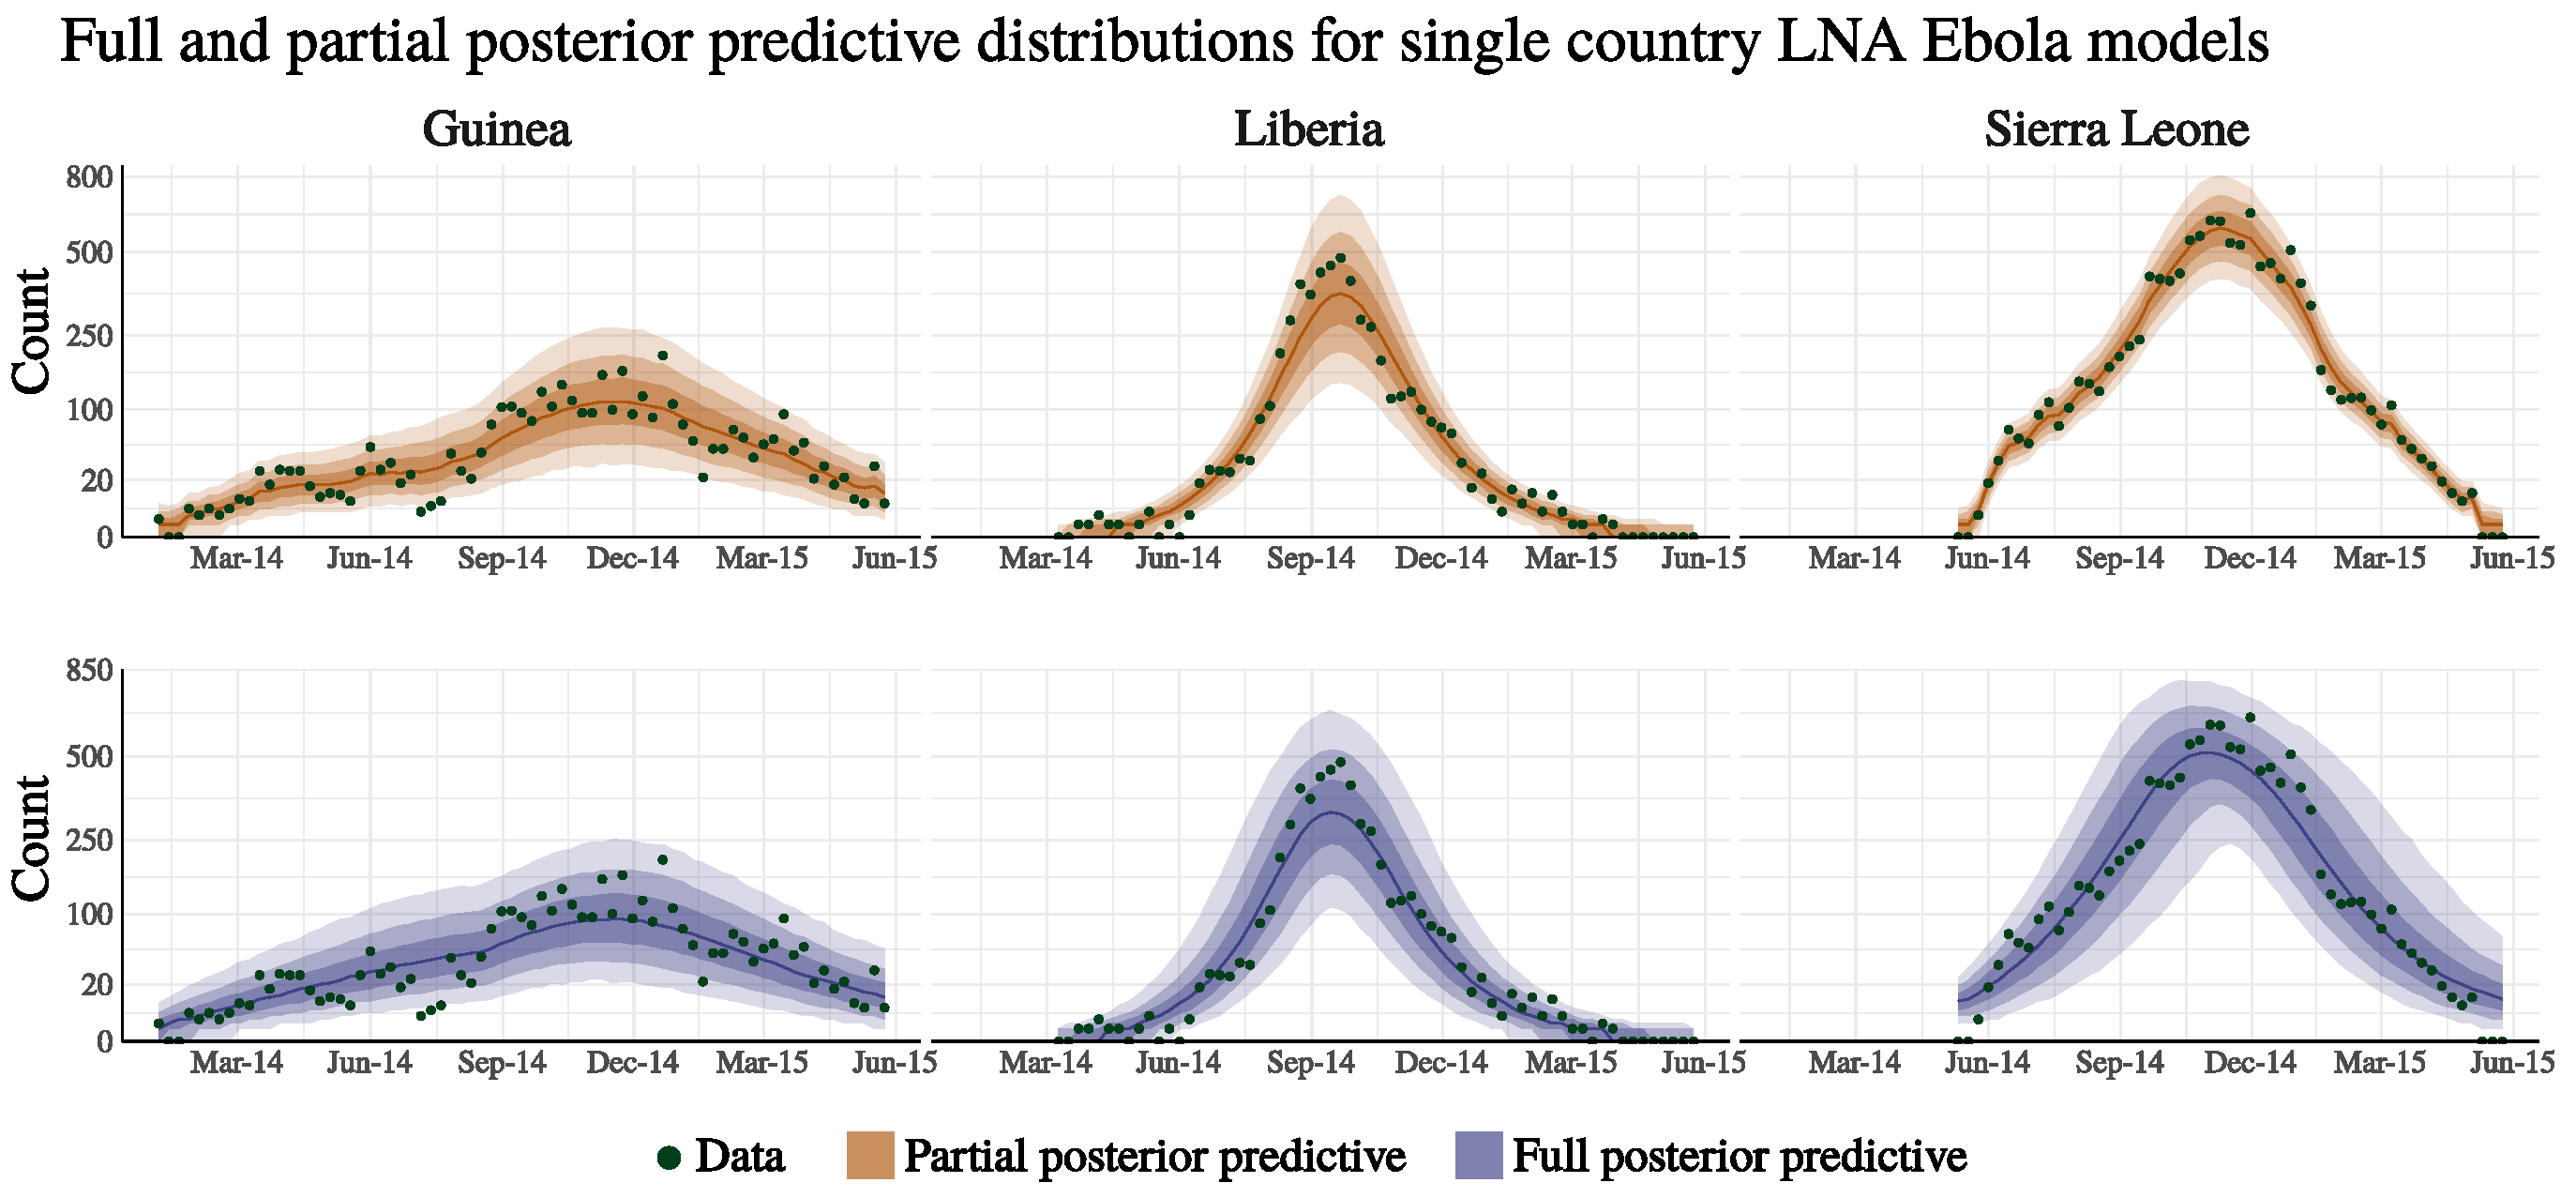
\includegraphics[width=0.9\linewidth]{figures/ebola_single_postpreds_lna}
		\caption[Posterior predictive distributions for country--specific SEIR LNA models for the West Africa Ebola outbreak.]{Partial and full posterior predictive distributions for country--specific SEIR LNA models for the West Africa Ebola outbreak. Green points correspond to the observed incidence. The shaded bands, in order of lightest to darkest, correspond to pointwise posterior 95\%, 80\%, and 50\% credible intervals, with the pointwise posterior median given by the corresponding colored solid line.}
		\label{fig:ebola_single_postpreds}
		
		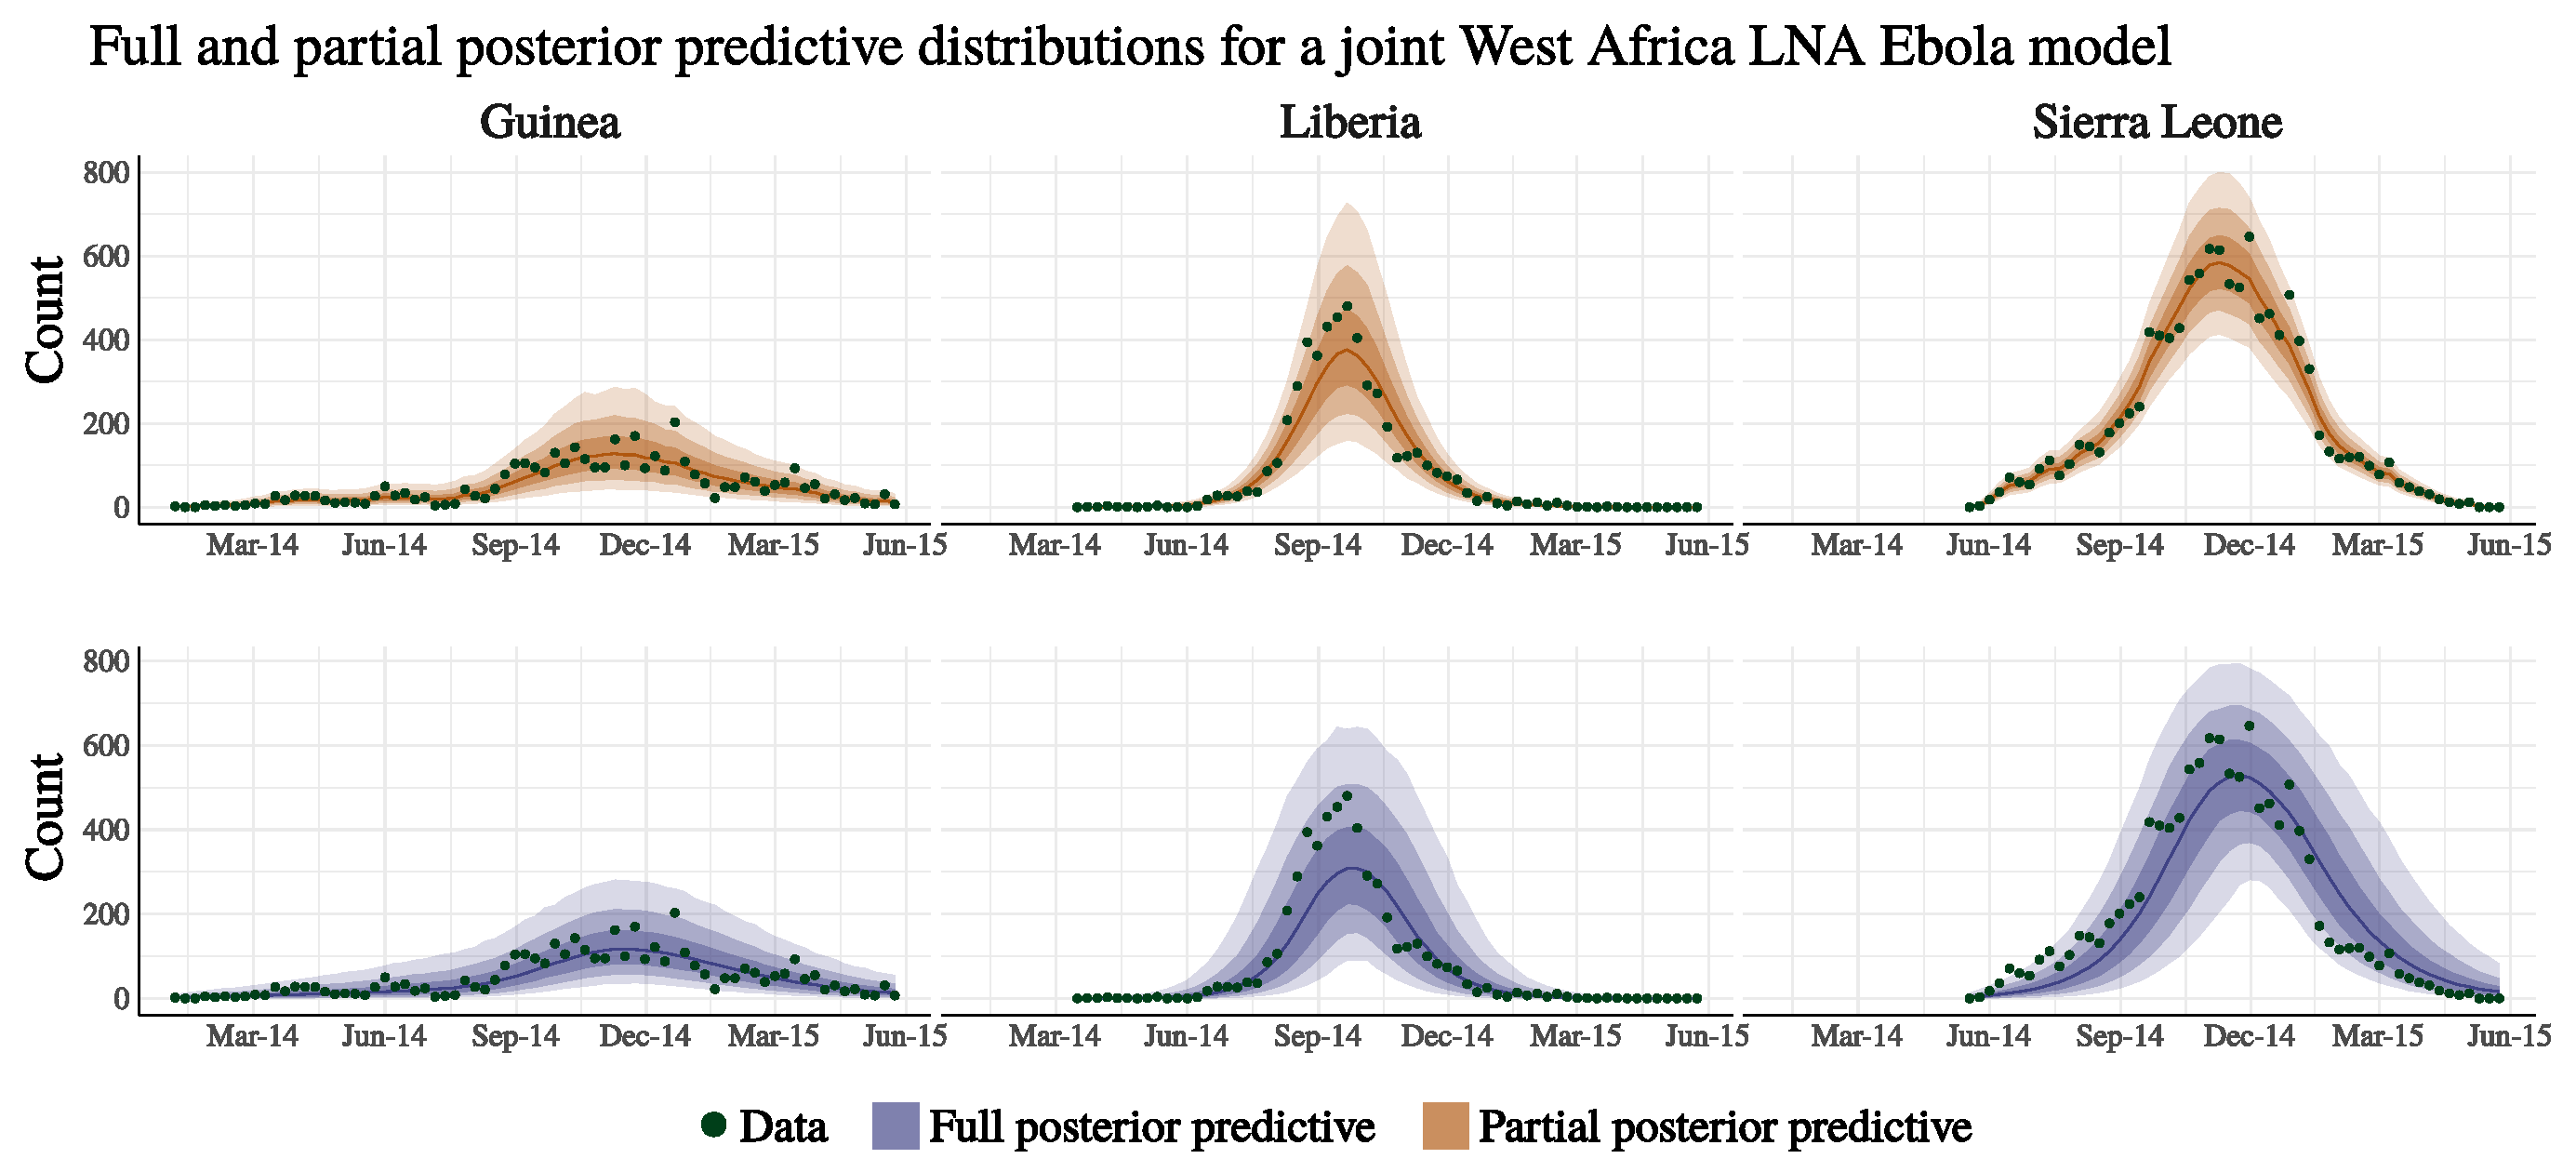
\includegraphics[width=0.9\linewidth]{figures/ebola_joint_postpreds_lna}
		\caption[Posterior predictive distributions for a stratified SEIR LNA model for the West Africa Ebola outbreak.]{Partial and full posterior predictive distributions for a stratified SEIR LNA model for jointly modeling the Ebola outbreak in West Africa. Green points correspond to the observed incidence. The shaded bands, in order of lightest to darkest, correspond to pointwise posterior 95\%, 80\%, and 50\% credible intervals, with the pointwise posterior median given by the corresponding colored solid line.}
		\label{fig:ebola_joint_postpreds}
\end{figure}

\subsubsection{Comparison with models fit via the ODE}
\label{subsubsec:ebola_lna_vs_ode}


\begin{figure}[htbp]
	\centering
	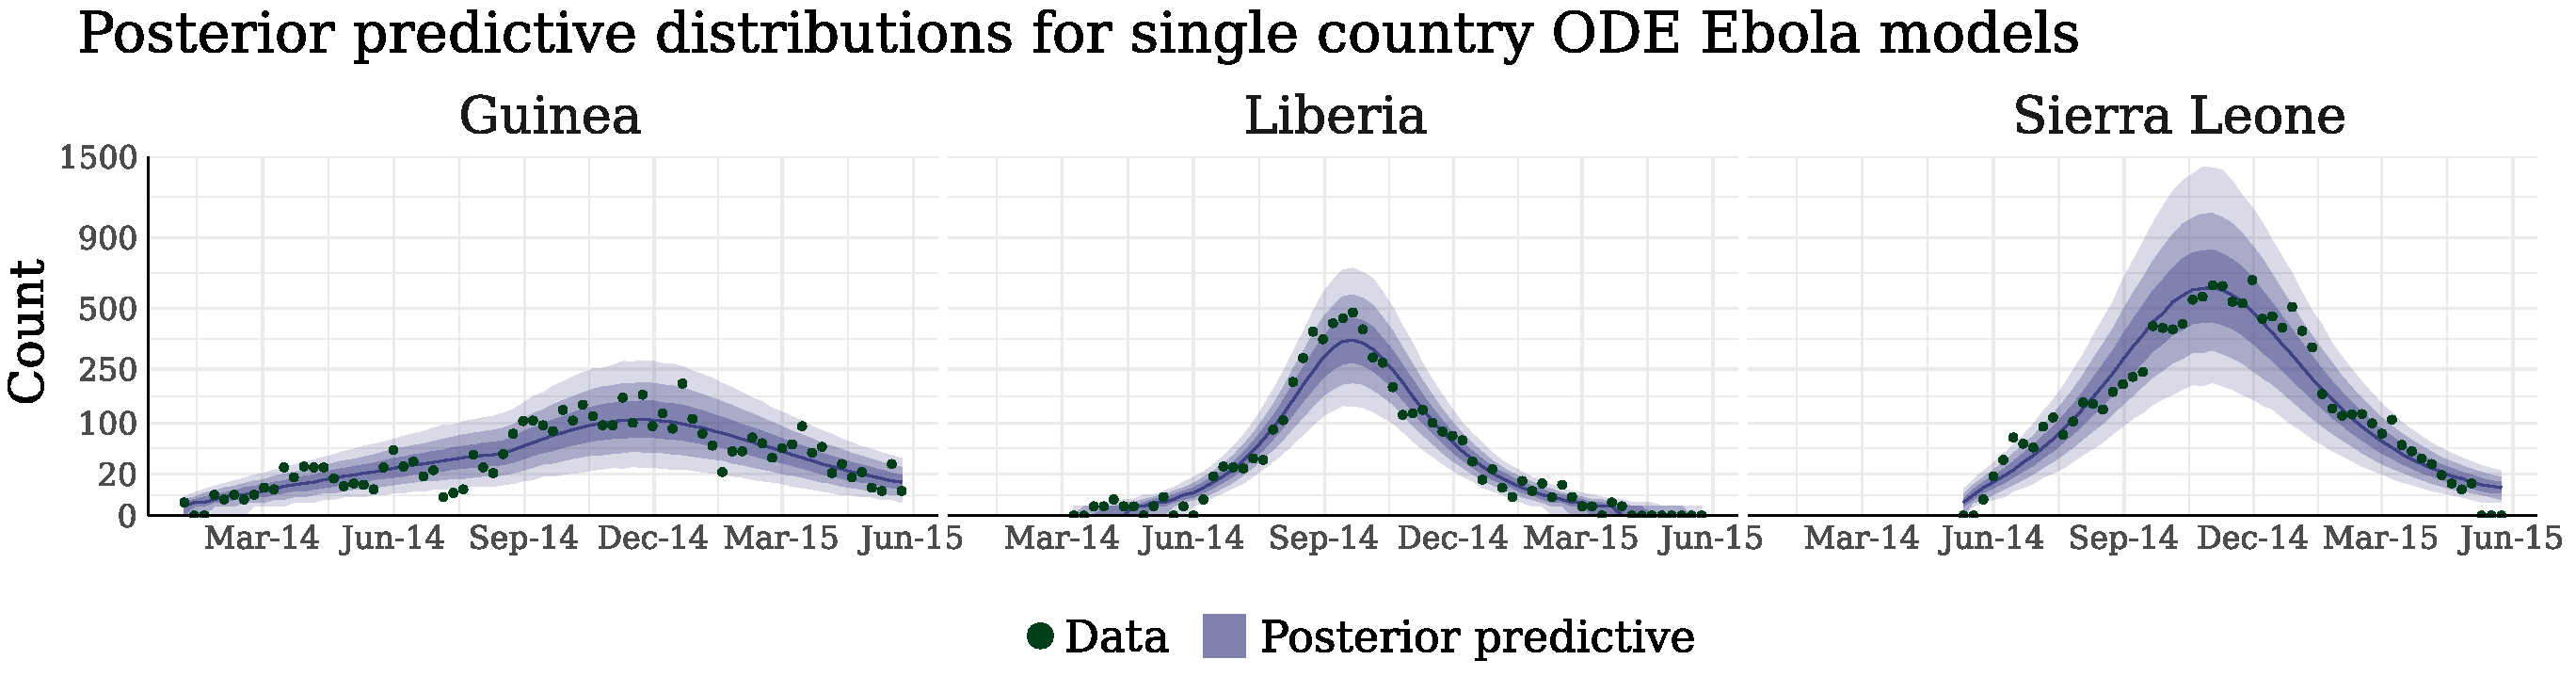
\includegraphics[width=\linewidth]{figures/ebola_single_postpreds_ode}
	\caption[Posterior predictive distributions for country--specific SEIR ODE models for the West Africa Ebola outbreak.]{Partial and full posterior predictive distributions for country--specific SEIR ODE models for the West Africa Ebola outbreak. Green points correspond to the observed incidence. The shaded bands, in order of lightest to darkest, correspond to pointwise posterior 95\%, 80\%, and 50\% credible intervals, with the pointwise posterior median given by the corresponding colored solid line.}
	\label{fig:ebola_single_postpreds_ode}
	
	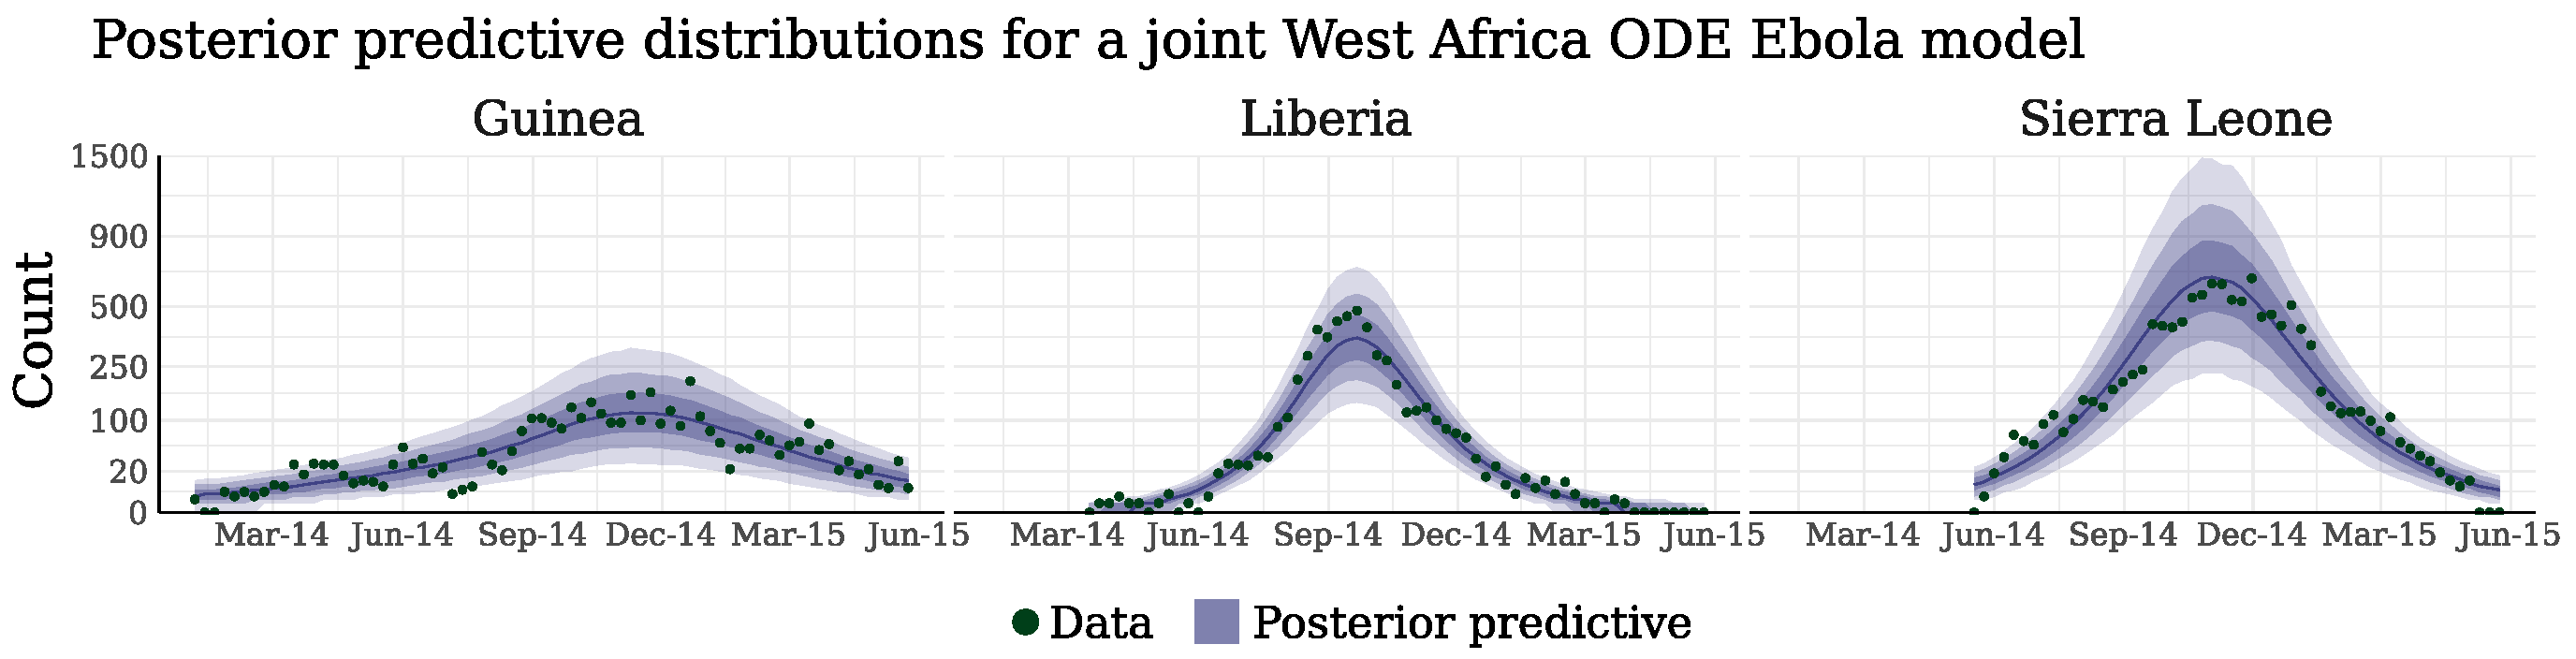
\includegraphics[width=\linewidth]{figures/ebola_joint_postpreds_ode}
	\caption[Posterior predictive distributions for a stratified SEIR ODE model for the West Africa Ebola outbreak.]{Partial and full posterior predictive distributions for a stratified SEIR ODE model for jointly modeling the Ebola outbreak in West Africa. Green points correspond to the observed incidence. The shaded bands, in order of lightest to darkest, correspond to pointwise posterior 95\%, 80\%, and 50\% credible intervals, with the pointwise posterior median given by the corresponding colored solid line.}
	\label{fig:ebola_joint_postpreds_ode}
\end{figure}

\newpage
\section{Discussion}
\label{sec:lna_discussion}

We have presented a framework for efficiently fitting SEMs to partially observed incidence data that is appropriate in large population settings where the time--evolution of the MJP can reasonably be approximated by LNA transition densities. The framework is neither specific to a particular set of model dynamics, nor is it dependent on the particular emission distributions that we used in the examples explored in this work. Therefore, it is possible to incorporate a SEM approximated via the LNA as part of a larger model in which multiple data streams, including incidence data, are synthesized to more precisely estimate the transmission dynamics of an outbreak. One advantage in our approach is that we can obtain approximate estimates of SEM parameters that appropriately account for the stochastic aspects of the MJP without resorting computationally intensive simulation--based methods. Thus, we are able to fit relatively complex models that are fully stochastic in all aspects of their transmission dynamics, such as the one used to jointly model the 2013--2016 outbreak of Ebola in Guinea, Liberia, and Sierra Leone. 

Our main contributions in this work were to demonstrate how a SEM can be reparameterized to admit latent epidemic paths that are compatible with emission distributions for incidence data, and how the LNA approximation can be reparameterized to take advantage of efficient MCMC machinery that can accommodate non--Gaussian emission distributions. We showed in simulations with simple SIR models, which are often used as building blocks in more complex models, that SEMs approximated via the LNA were comparable to those approximated using MMTL, and vastly outperformed ODE approximations that are still in common use. Moreover, the computational advantage of the LNA allowed us to fit a relatively complex model, that we were unable to fit using MMTL within a pseudo--marginal framework, to data from the Ebola outbreak in West Africa. We also presented a handful of interpretable and easily implemented model diagnostics.  

While this work has addressed various aspects of how to efficiently fit models that can be used to describe the transmission dynamics of an outbreak, there are also several important issues regarding the application and scientific validity of these models that we have not addressed in depth. Critically, it is frequently, if not universally, unreasonable to assume that the transmission and surveillance dynamics are constant over time. We will address this issue in the next chapter, where we will fit models with time--varying dynamics. Other topics that we have not covered, in part because of the complexity and breadth of the work already presented here, are formal assessments of the predictive performance, issues of model selection, and the effects of model misspecification beyond the use of the LNA to approximate the MJP representation of a SEM.